\documentclass[12pt,a4paper, usenames, dvipsnames]{article}
\usepackage{graphicx}
\usepackage{xcolor}


\usepackage[ngerman]{babel}
\usepackage[utf8]{inputenc}
\usepackage{mathtools}
\usepackage{amsmath}
\usepackage{amssymb}
\usepackage{geometry}
\usepackage{tikz}
\usepackage{float}
\usepackage{verbatim}

\usepackage{amsthm}


\newtheoremstyle{mystyle}% name
{15pt}% Space above
{5pt}% Space below
{\itshape}% Body font
{}% Indent amount: 
{\bf}% Theorem head font
{}% Punctuation after theorem head
{\newline}% Space after theorem head
{}% Theorem head 

\theoremstyle{mystyle}
\newtheorem{definition}{Definition}


\newtheoremstyle{definition}% name
{15pt}% Space above
{5pt}% Space below 
{}% Body font
{}% Indent amount: Indent amount: empty = no indent, \parindent = normal paragraph indent
{\bf}% Theorem head font
{}% Punctuation after theorem head
{\newline }% Space after theorem head: Space after theorem head: { } = normal interword space; \newline = linebreak
{}% Theorem head spec (can be left empty, meaning `normal')

\theoremstyle{definition}

\newtheorem{bsp}{Beispiel}[definition]

\usepackage[nottoc]{tocbibind}

\usepackage[onehalfspacing]{setspace}

\usepackage{stmaryrd}

\usepackage{microtype}

\usepackage{booktabs}

\usepackage{array}

\usepackage{hyperref}
\hypersetup{
    colorlinks=true,
    linkcolor=black,
    filecolor=black,      
    urlcolor=blue,
    citecolor=black
}

\usepackage{subfigure}

\usepackage[compact]{titlesec}     


\usepackage[center]{caption}


\pagestyle{plain}

\usepackage[backend=biber]{biblatex}

\addbibresource{references.bib}

\usepackage{adjustbox}

\newcommand{\Gtwo}{\ensuremath{G_{2\times 2\times 2}}}

\newcommand{\Gthree}{\ensuremath{G_{3\times 3\times 3}}}

\newcommand{\Ttwo}{2$\times$2$\times$2-}

\newcommand{\Tthree}{3$\times$3$\times$3-}

\clubpenalty = 10000
\widowpenalty = 10000
\displaywidowpenalty = 10000


\geometry{
  paper=a4paper, % Change to letterpaper for US letter
  top=3cm, % Top margin
  left=2cm, % Left margin
  right=3cm, % Right margin
  %showframe, % Uncomment to show how the type block is set on the page
}

\setlength{\parindent}{0em}

\setlength{\parskip}{1.3ex}

\pagenumbering {arabic} 

\titlespacing*{\section}{0pt}{10ex plus 1ex minus .2ex}{4.3ex plus .2ex}









\begin{document}

\pagenumbering{roman}


\begin{titlepage}
	\centering
	{\scshape\LARGE Technische Universität Dortmund \par}
	Fakultät für Informatik \par
	Lehrstuhl 14 für Software Engineering \par
	\vspace{1cm}
	{\scshape\Large Bachelorarbeit \par }
	\vspace{1.5cm}
	{\huge\bfseries  Gruppentheorie des \\ 2$\times$2$\times$2 Zauberwürfels und dessen Lösungsalgorithmen \par}
	\vspace{2cm}
	{\Large\itshape Pina Kolling\par}
	\vspace{0.5cm}
	{Abgabe: Mai 2021 \par }
	\vfill
	betreut von\par
	Dr. \L ukasz \textsc{Czajka} \par 
	und \par 
	M. Sc. Christoph \textsc{Stahl} 

	\vfill

% Bottom of the page
	{\large \today\par}
\end{titlepage}

\setcounter{page}{2}

\begin{singlespace}
\tableofcontents

\end{singlespace}





\newpage

\pagenumbering{arabic}

\setcounter{page}{1} 
%

%
%
%
%
%=======================================================================================================
%
%
%
%
%
\section{Einleitung}

\label{Kapitel_Einleitung}

Der \Tthree Zauberwürfel ist ein mathematisches Drehpuzzle, das 1974 von dem ungarischen Professor Er\~{n}o Rubik erfunden wurde. Er wollte damit seinen Studenten helfen, dreidimensionale Probleme zu verstehen. Er\~{n}o Rubik selbst brauchte über einen Monat, um den \Tthree Würfel zum ersten Mal zu lösen.
Der sogenannte \textit{Rubik's Cube} wurde ab 1980 weltweit verkauft und 1982 fand in Budapest sogar die erste Weltmeisterschaft statt. Der Gewinner war Minh Thai aus den USA, der den Würfel in $22,95$ Sekunden löste. \cite{RC} Im Jahr 2018 löste der Chinese Yusheng Du den Würfel bei einem Wettbewerb in $3,47$ Sekunden und stellte damit einen neuen Rekord auf. \cite{rekord}
Das Patent für den kleineren \Ttwo Würfel hat \textit{Rubik} im Jahr 1981 angemeldet \cite{patent}. Um diesen Würfel geht es in dieser Arbeit.

Doch die Zauberwürfel sind nicht nur interessante Puzzle -- sie bieten beispielsweise auch die Möglichkeit, sie maschinell mit Bild- und Farberkennung zu lösen. Außerdem können die Würfel als algebraische Strukturen dargestellt werden.

%
%
%
%
%=======================================================================================================
%
%
%
%
\subsection*{Motivation} \addcontentsline{toc}{subsection}{\protect\numberline{}Motivation}




Der \Tthree Würfel wurde mathematisch schon viel untersucht. 
Die \textit{God's Number} -- das ist die maximal mögliche Anzahl der nötigen Drehungen zur Lösung -- wurde oft berechnet und durch neue Algorithmen verbessert. 
Die Berechnung der \textit{God's Number} des \Tthree Würfels ist wesentlich anspruchsvoller und dadurch auch interessanter als die des \Ttwo Würfels. 

Auch als Gruppe wurde der \Tthree Würfel schon mehrfach dargestellt, während der \Ttwo Würfel
noch nicht umfangreich als Gruppe untersucht wurde. Ziel dieser Arbeit ist es, das Wissen des \Tthree Würfels auf den \Ttwo Würfel zu übertragen. Der \Ttwo Würfel hat im Gegensatz zum \Tthree Würfel weniger Steine und keine Kantsteine -- dadurch ist der kleinere Würfel auch weniger komplex. Dafür kann der \Ttwo Würfel aber aufgrund der fehlenden Mittelsteine rotiert werden und so kann die Oberseite beliebig geändert werden. In dieser Arbeit wird das Wissen der Gruppe des \Tthree Würfels übertragen und angepasst und somit der \Ttwo Würfel mit der Gruppentheorie dargestellt.

Wer die Lösungsalgorithmen des \Ttwo Zauberwürfels selber herleiten möchte, sollte dies vor dem Lesen dieser Arbeit tun, da diese hier teilweise erklärt und genutzt werden.

%
%
%
%
%=======================================================================================================
%
%
%
%
\subsection*{Struktur} \addcontentsline{toc}{subsection}{\protect\numberline{}Struktur}

Diese Arbeit setzt sich aus 9 Kapiteln zusammen. Im Folgenden werden die Inhalte und Themen dieser Kapitel aufgelistet.

\begin{itemize}
\item[\textbf{\ref{Kapitel_Einleitung}}] In der Einleitung wird eine kurze Übersicht der Geschichte des Würfels gegeben. Außerdem befinden sich hier die Motivation und die Struktur.

\item[\textbf{\ref{Kapitel_Würfel}}] In diesem Kapitel wird der Aufbau des \Ttwo Würfels und die dazugehörige Terminologie erklärt. Außerdem werden die Grundzüge des Würfels definiert.

\item[\textbf{\ref{Kapitel_MathematischeGrundlagen}}] Hier werden die mathematischen Grundlagen erklärt. Dafür werden unter anderem Gruppen und andere algebraische Strukturen definiert und anhand von Beispielen erklärt.

\item[\textbf{\ref{Kapitel_KonfigurationDesWürfels}}] In dem Kapitel \textit{Konfiguration des Würfels} werden die Positionen der Steine und die Ausrichtung der Steine im Würfel erklärt. Daraus setzt sich die Konfiguration zusammen. 

\item[\textbf{\ref{Kapitel_WürfelAlsGruppe}}] In diesem Kapitel wird die Gruppe des \Ttwo Würfels beschrieben. Außerdem werden Äquivalenzrelationen eingeführt, um die Rotationen des Würfels zu realisieren.

\item[\textbf{\ref{Kapitel_Untergruppen}}] Das Kapitel \textit{Untergruppen} befasst sich mit Beispieluntergruppen, Erzeugern und Cayleygraphen der Gruppe des\Ttwo Würfels.

\item[\textbf{\ref{Kapitel_ValideKonfigurationen}}] Hier wird die Anzahl der möglichen Würfelkonfigurationen und die Mächtigkeit der Trägermenge der Gruppe des \Ttwo Würfels berechnet.

\item[\textbf{\ref{Kapitel_Lösung}}] In diesem Kapitel werden verschiedene Lösungsansätze und Algorithmen erklärt. Die Lösung des Wüfels durch einen Menschen wird schrittweise erklärt und es gibt eine allgemeine Anleitung, mit der der \Ttwo Würfel immer gelöst werden kann.

\item[\textbf{\ref{Kapitel_Fazit}}] Am Schluss der Arbeit befindet sich die Zusammenfassung, das Ergebnis und der Ausblick.

\end{itemize}


%
%
%
%
%
%
%=======================================================================================================
%
%
%
%
%
%
\newpage
\section{Der \Ttwo Würfel}

\label{Kapitel_Würfel}

In diesem Kapitel werden die Grundlagen des \Ttwo \textit{Cubes} erklärt. Zuerst wird der Aufbau und die Terminologie des Würfels erläutert. Dann wird kurz auf die Unterschiede zwischen dem \Ttwo und dem \Tthree Würfel eingegangen. 
Außerdem werden die sechs Grundzüge des Würfels definiert und erklärt. Darauf basieren alle späteren Algorithmen. 


%
%
%
%
%
%
%=======================================================================================================
%
%
%
%
\subsection*{Terminologie} \addcontentsline{toc}{subsection}{\protect\numberline{}Terminologie}

Diese Arbeit befasst sich mit dem \Ttwo Zauberwürfel, deshalb sind die Terminologie und der Aufbau des \textit{Cubes} Grundlagen für die weiteren Kapitel.
Im Folgenden wird die Terminologie und der Aufbau des Würfels erklärt.



\begin{description}


\item[\Ttwo Würfel] (auch Zauberwürfel oder \textit{Cube}) 

Der Würfel setzt sich aus acht kleinen Würfeln zusammen.
In Abbildung \ref{Abbildung_WürfelUngelöstGelöst} ist er links verdreht und rechts im gelösten Zustand zu sehen. Der gelöste Zustand wird auch als Startkonfiguration bezeichnet.
Bei der Startkonfiguration (auch Grundposition, Grundstellung) des \Ttwo Würfels hat jede Seite 4 Farbflächen einer Farbe. Der Würfel ist dann gelöst.  
Bei dem verdrehten Würfel können die Steine des Würfels an anderen Positionen sein und anders ausgerichtet sein.
\begin{figure}[h]
\centering
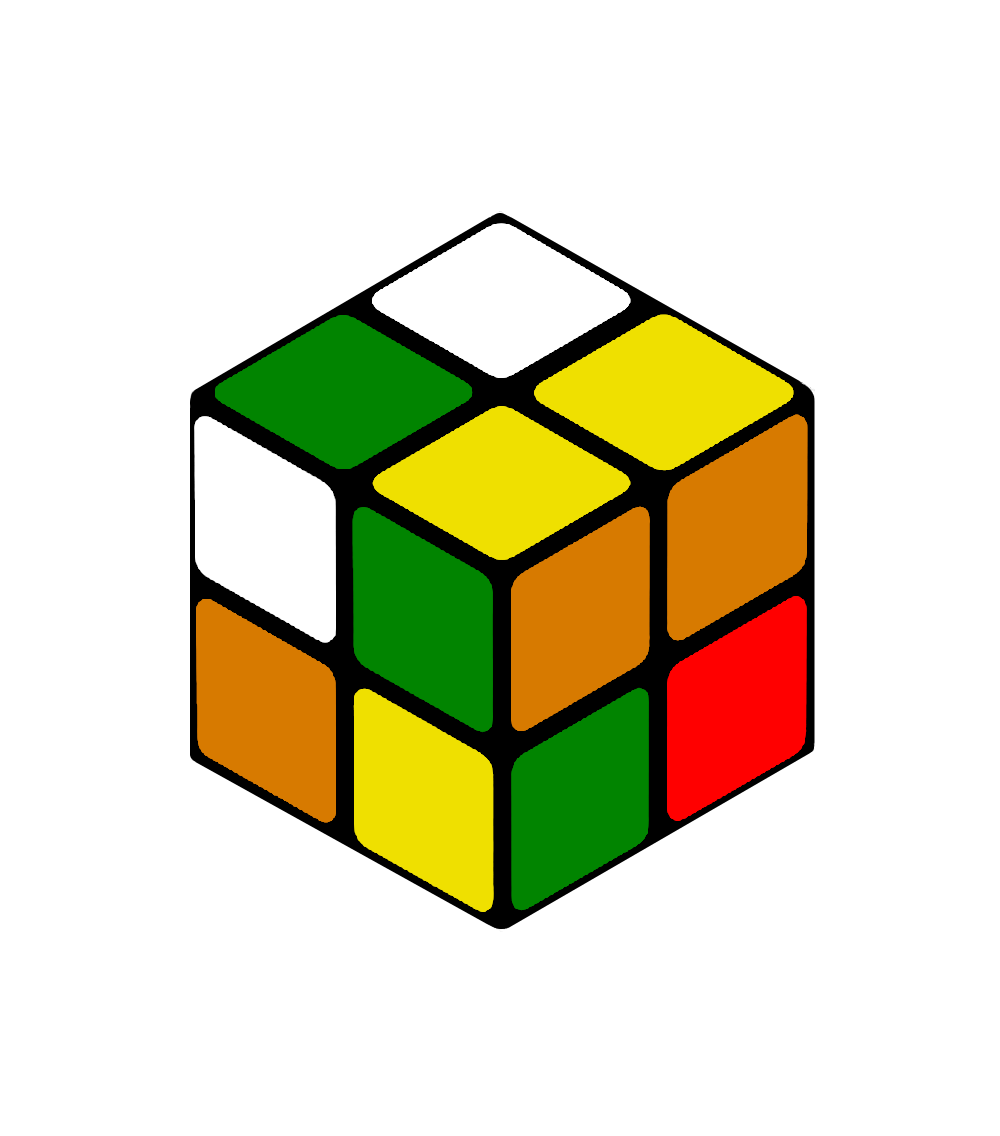
\includegraphics[scale=0.1]{2x2scrambled.png}
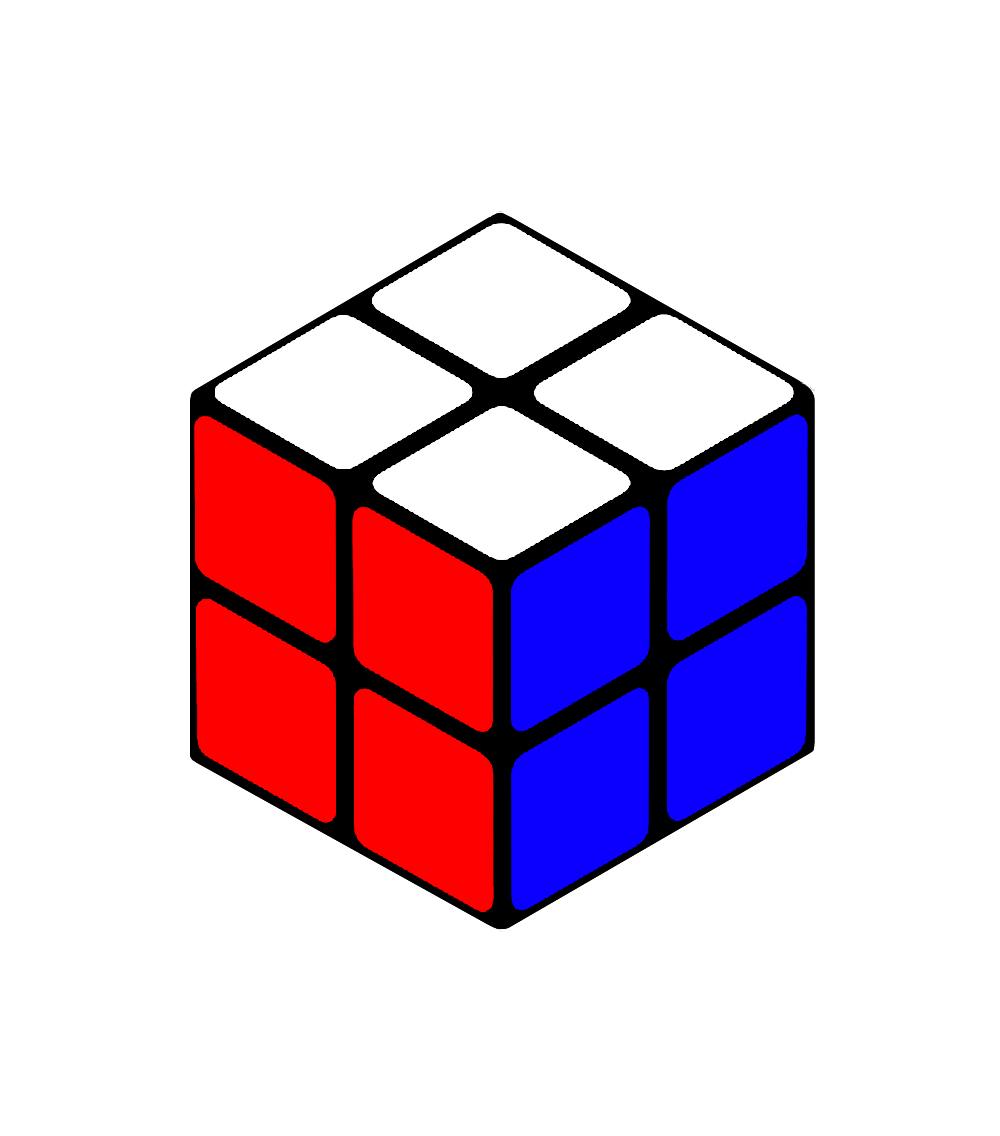
\includegraphics[scale=0.1]{2x2solved.png}
\caption[ungelöster und gelöster \Ttwo Würfel]{ungelöster und gelöster \Ttwo Würfel}
\label{Abbildung_WürfelUngelöstGelöst}
\end{figure}


\item[Eckstein und Farbfläche] \ \\
Ein \Ttwo Würfel besteht aus acht Ecksteinen (links in Abbildung \ref{Abbildung_Eckstein}), die jeweils drei Farbflächen (rechts in Abbildung \ref{Abbildung_Eckstein}) haben. Ein \Ttwo Zauberwürfel hat somit 24 Farbflächen. Die verschiedenen Farbpaare, die sich jeweils gegenüberliegen, sind weiß und gelb, rot und orange, grün und blau.
\begin{figure}[h]
\centering
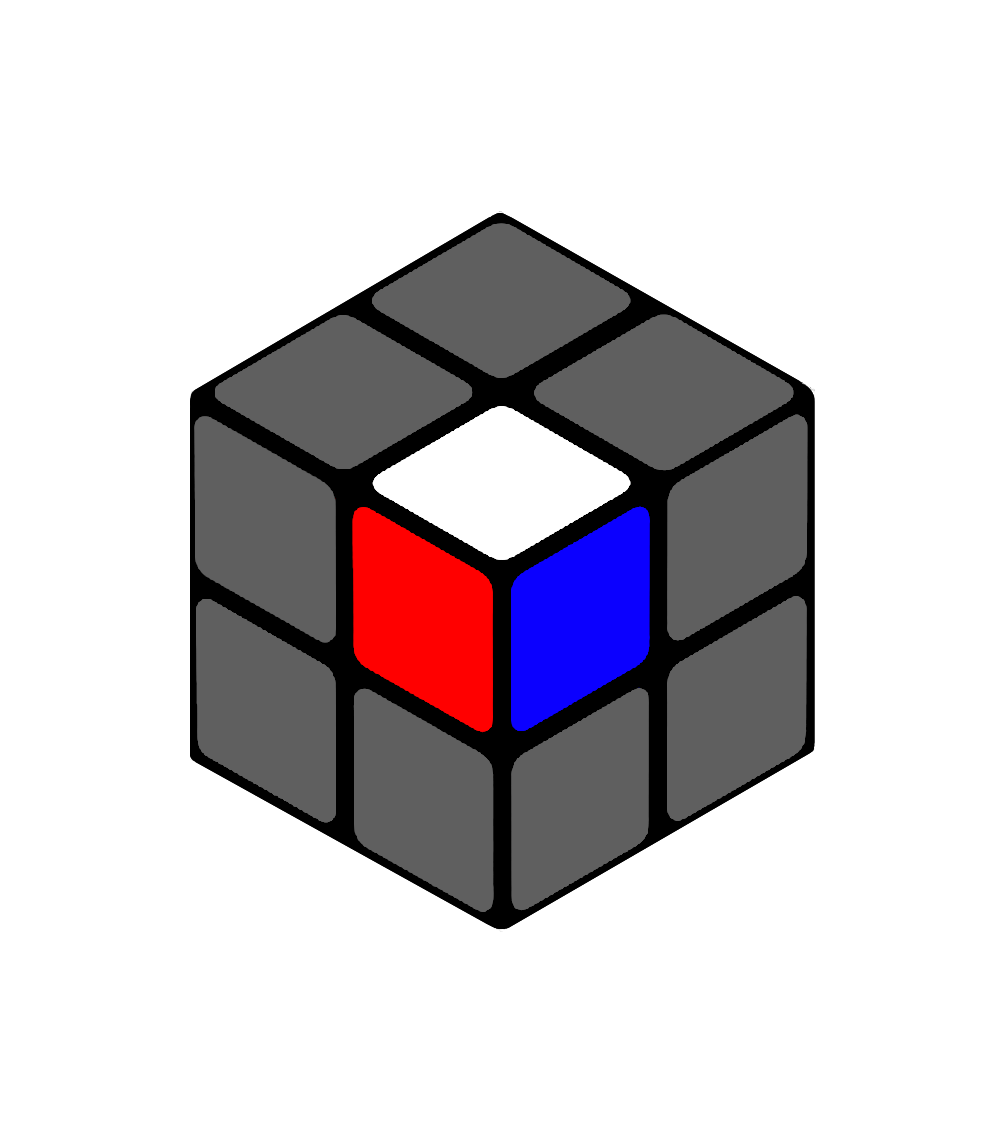
\includegraphics[scale=0.1]{2x2stein.png}
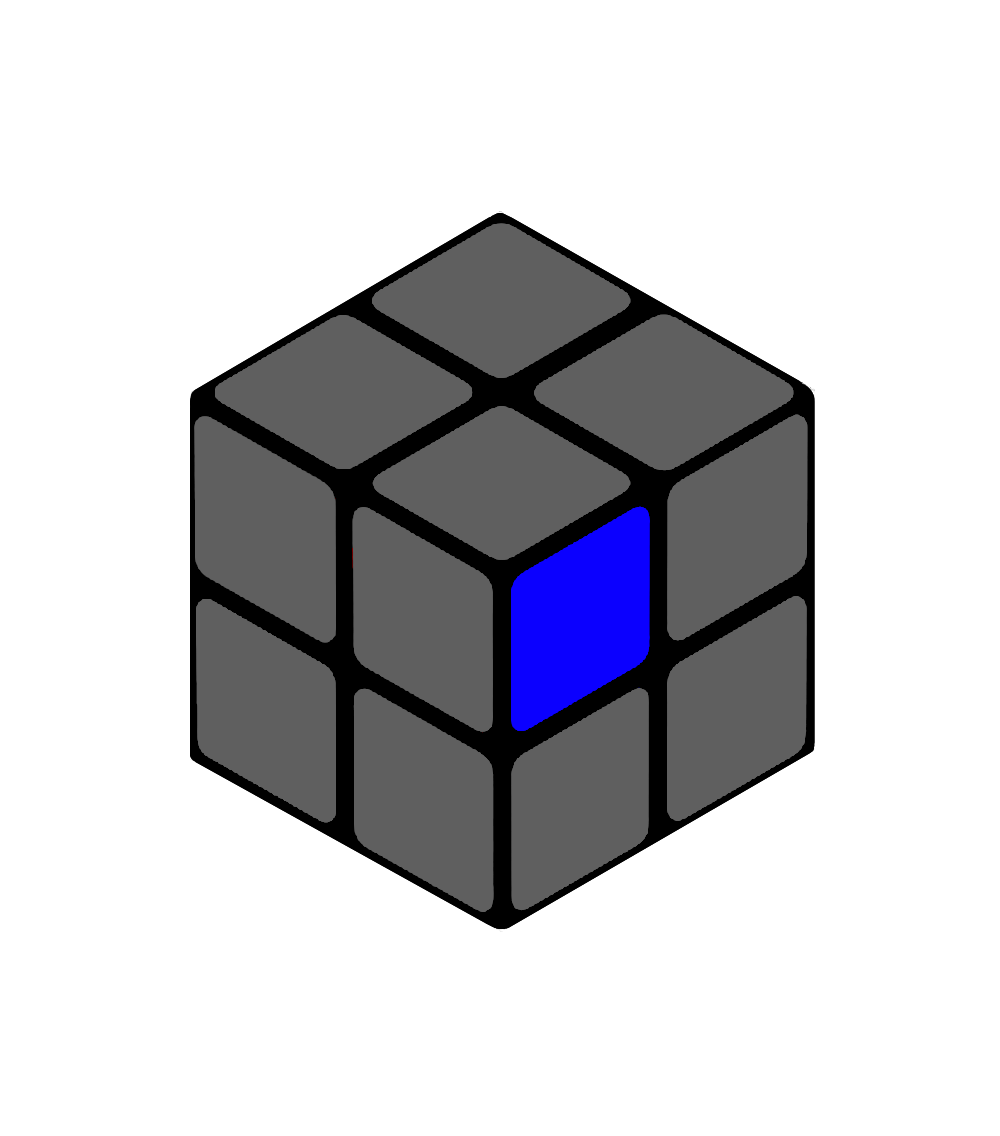
\includegraphics[scale=0.1]{2x2farbflaeche.png}
\caption[Eckstein und Farbfläche des Würfels]{Eckstein und Farbfläche des Würfels}
\label{Abbildung_Eckstein}
\end{figure} 


\newpage

\item[Seite] \ \\
Der \Ttwo und der \Tthree Würfel haben sechs Seiten (bestehend aus jeweils vier Farbflächen) und somit sechs Farben. Die weiße Seite wird üblicherweise als obere Seite bezeichnet. Für den Machanismus ist die Ausrichtung des Würfels aber nicht relevant.

\begin{figure}[h]
\centering
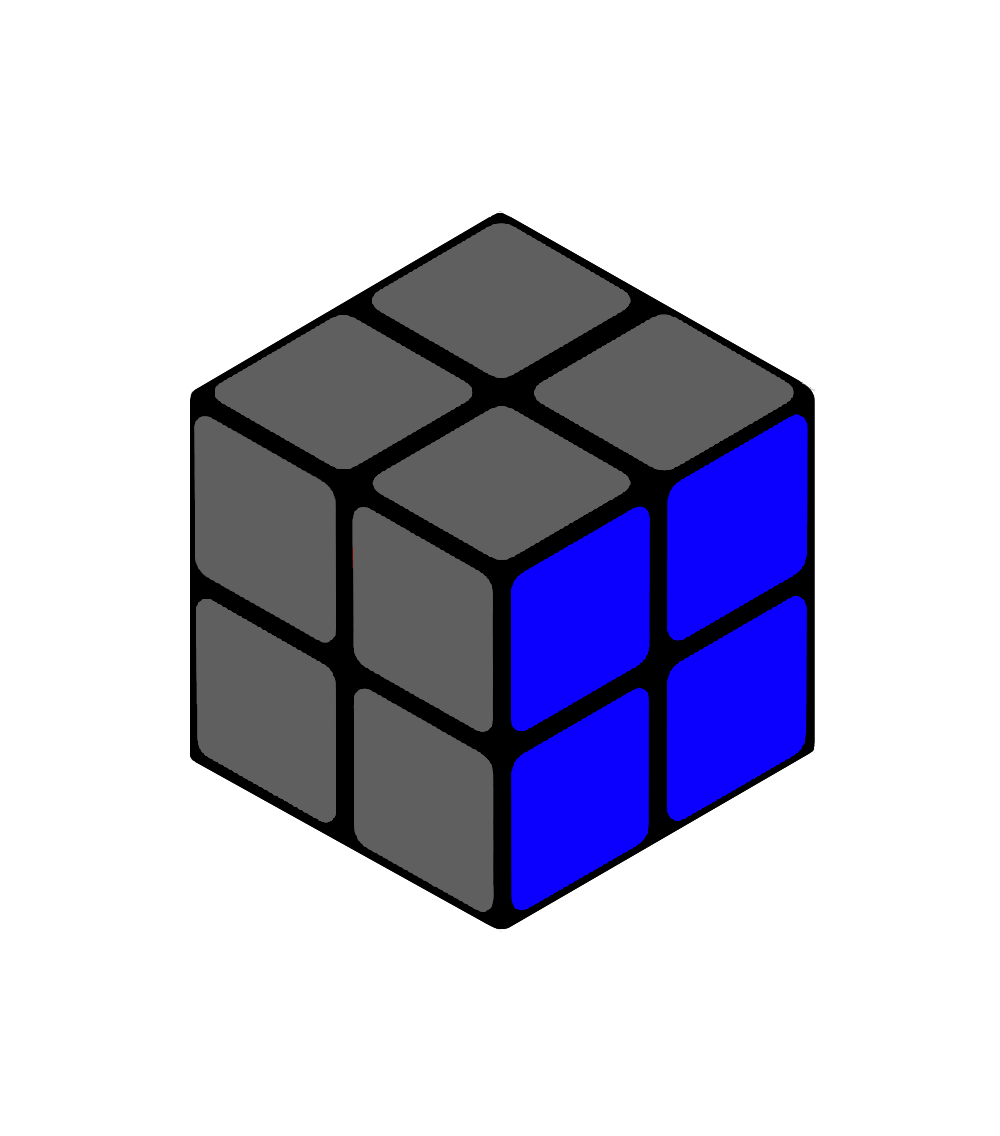
\includegraphics[scale=0.1]{2x2seite.png}
\caption[Seite des Würfels]{Seite des Würfels}
\end{figure}


\item[\Tthree Würfel] \ \\
Wesentlich bekannter als der \Ttwo \textit{Cube} ist der \Tthree \textit{Cube}. Er besteht aus 26 Steinen. In Abbildung \ref{Abbildung_3erWürfel} ist er links ungelöst und rechts in der Startkonfiguration zu sehen.

\begin{figure}[h]
\centering
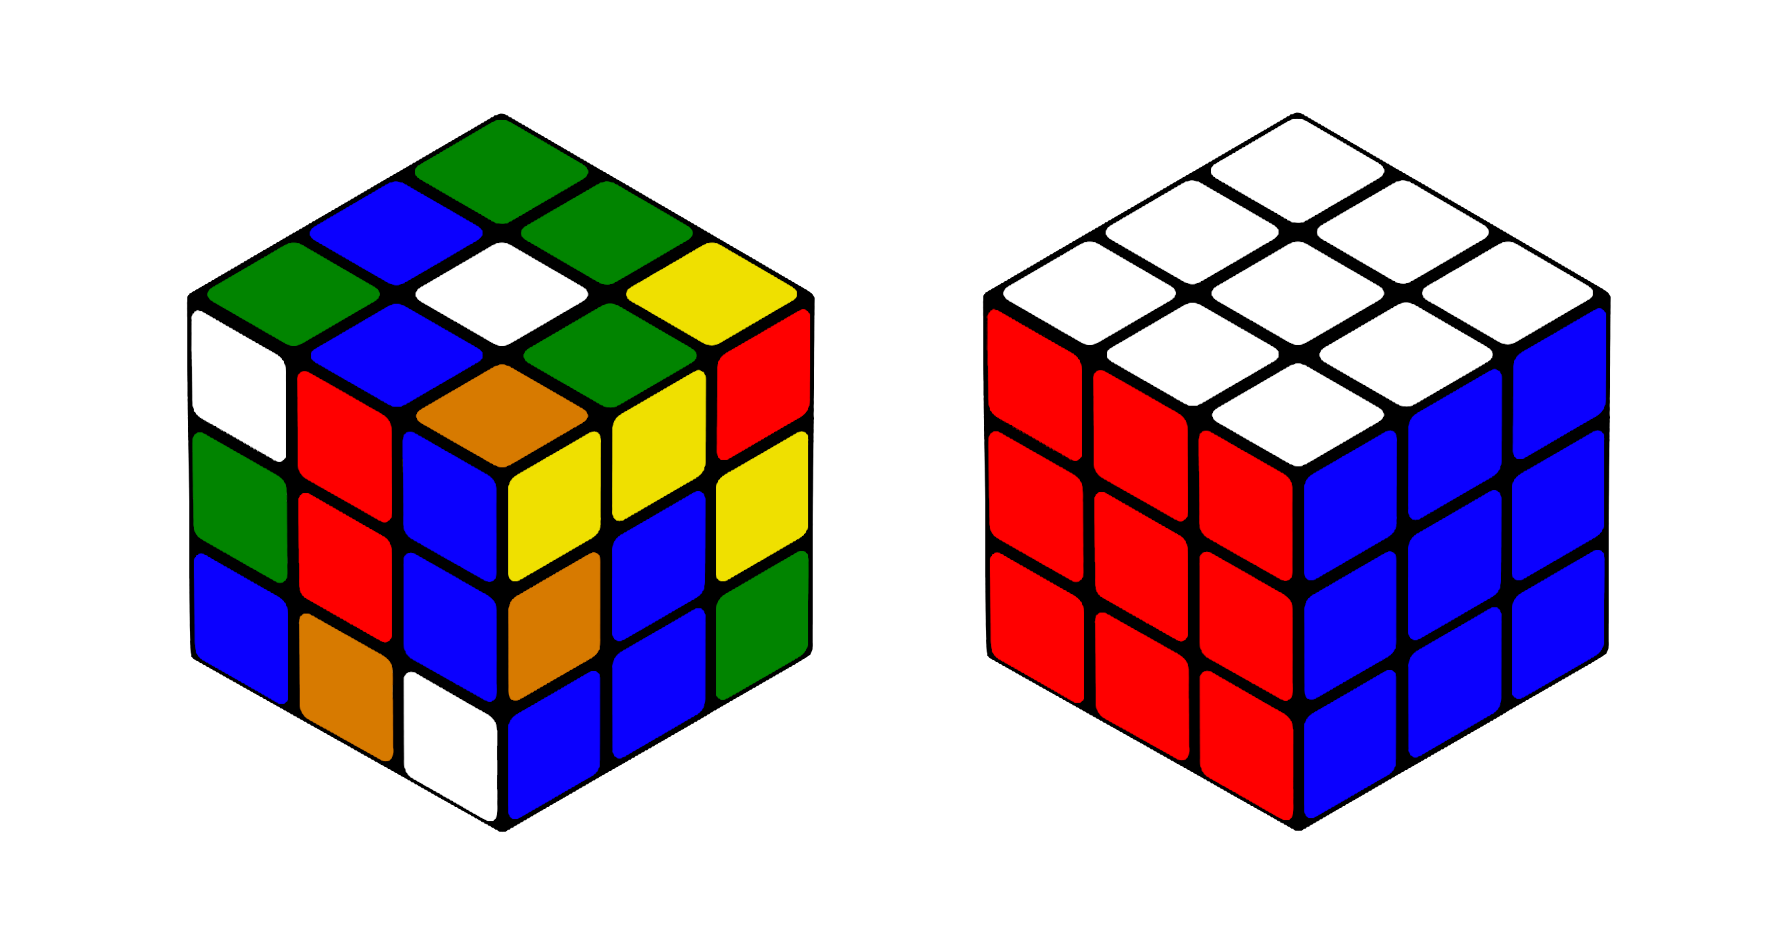
\includegraphics[scale=0.11]{3x3_sc_so.png}
\caption[ungelöster und gelöster \Tthree Würfel]{ungelöster und gelöster \Tthree Würfel}
\label{Abbildung_3erWürfel}
\end{figure}

\newpage
\item[Mittel- und Kantsteine] \ \\
Im Gegensatz zum \Ttwo \ hat der \Tthree Würfel Kantsteine und Mittelsteine (s. Abbildung \ref{Abbildung_MittelKantSteine}).
Das Besondere an den Mittelsteinen des \Tthree Würfels ist, dass sie bei einer Drehung der Ebenen (also bei Zügen des Würfels) nicht verändert werden. Somit ist beim \Tthree Würfel die obere Seite immer fest zu stellen: Die obere Seite hat immer das weiße Mittelstück in der Mitte. 
\begin{figure}[H]
\centering
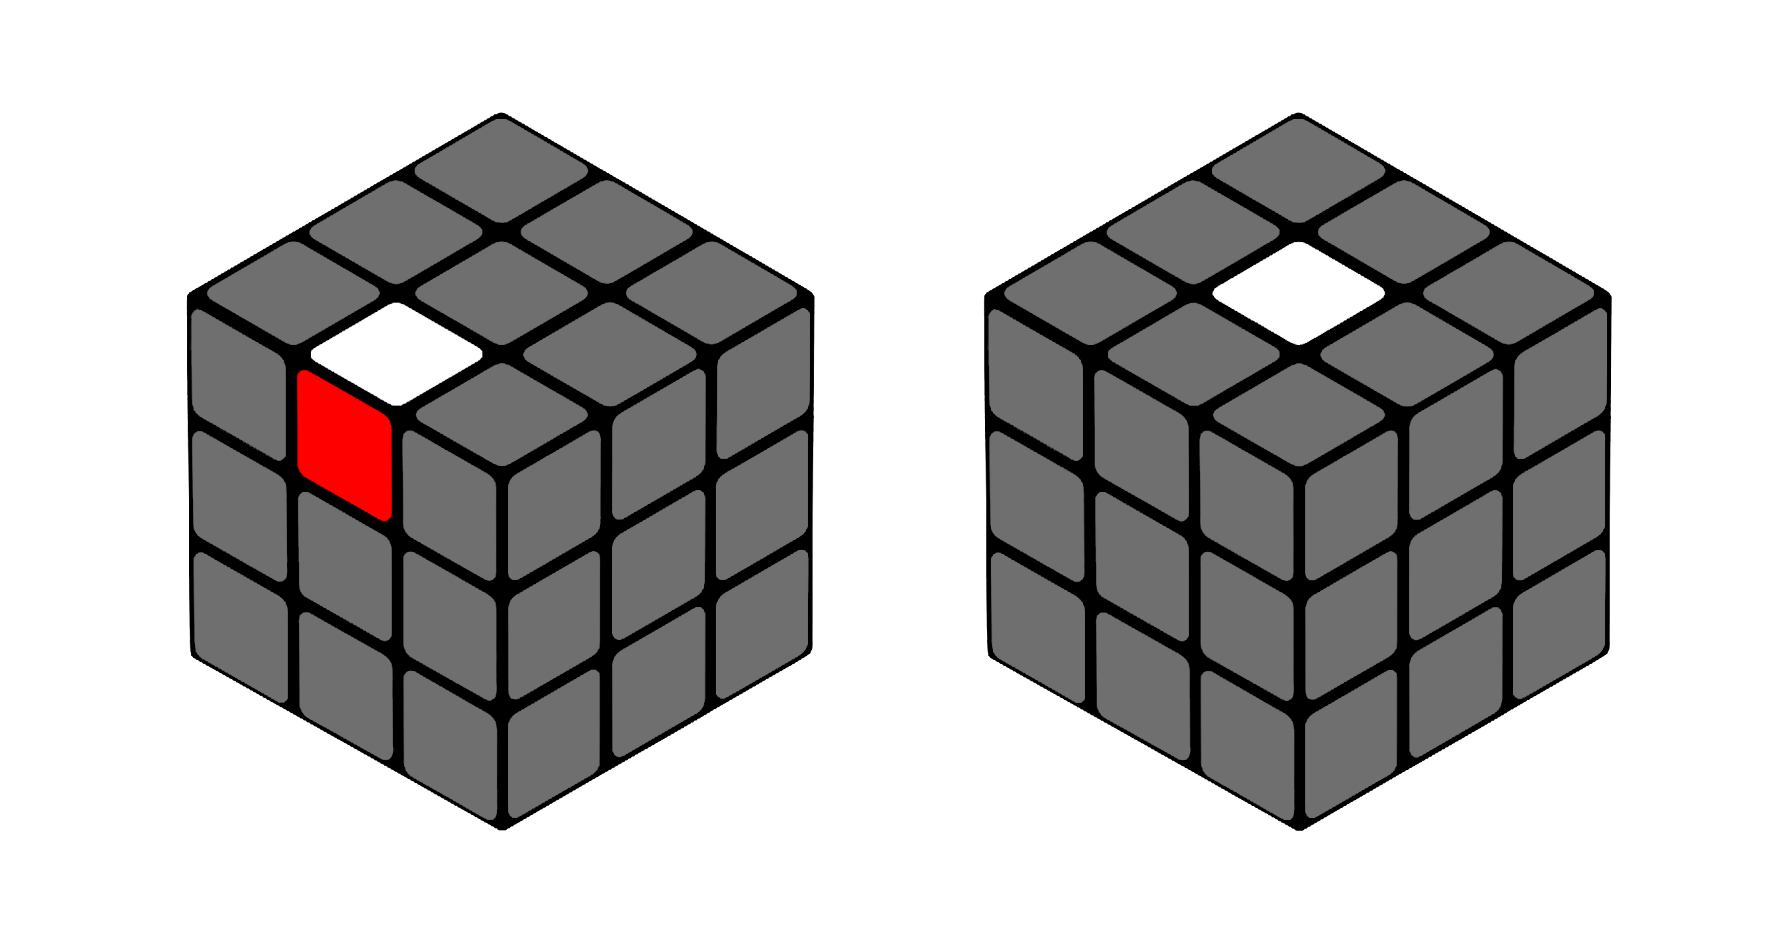
\includegraphics[scale=0.11]{mittelkant.png}
\caption[Kant- und Mittelsteine]{Kant- und Mittelsteine}
\label{Abbildung_MittelKantSteine}
\end{figure}



\end{description}

Beim \Ttwo \textit{Cube} gibt es keine eindeutige Oberseite. Es ist dementsprechend möglich, dass die aktuelle Konfiguration einer vermeintlich anderen Konfiguration entspricht, bei der nur eine andere Seite nach oben gehalten wird.
Die Ausrichtung des gesamten Würfels ist bei dem \Tthree Würfel also eindeutig vorgegeben, während sie beim \Ttwo Würfel gedreht werden kann.  
Das muss beachtet werden, da in dieser Arbeit die Gruppentheorie des \Tthree \textit{Cubes} auf den \Ttwo Würfel übertragen wird. Es wird sich dabei vorallem an \textit{Group Theory an the Rubik's Cube} von Janet Chen \cite{JC} und \textit{Group Theory via Rubik's Cube} von Tom Davis \cite{TD} orientiert.

%
%
%
%
%
%
%
%=======================================================================================================
%
%
%
%
%
%


\subsection*{Grundzüge des Würfels} \addcontentsline{toc}{subsection}{\protect\numberline{}Grundzüge des Würfels}
\label{Abschnitt_GrundzügeWürfel}
Am \Ttwo Zauberwürfel gibt es sechs verschiedene Drehseiten (auch Ebenen): oben, unten, links, rechts, vorne und hinten. 
In Abbildung \ref{Abbildung_Ebene} ist die obere Ebene markiert.

\begin{figure}[H]
\centering
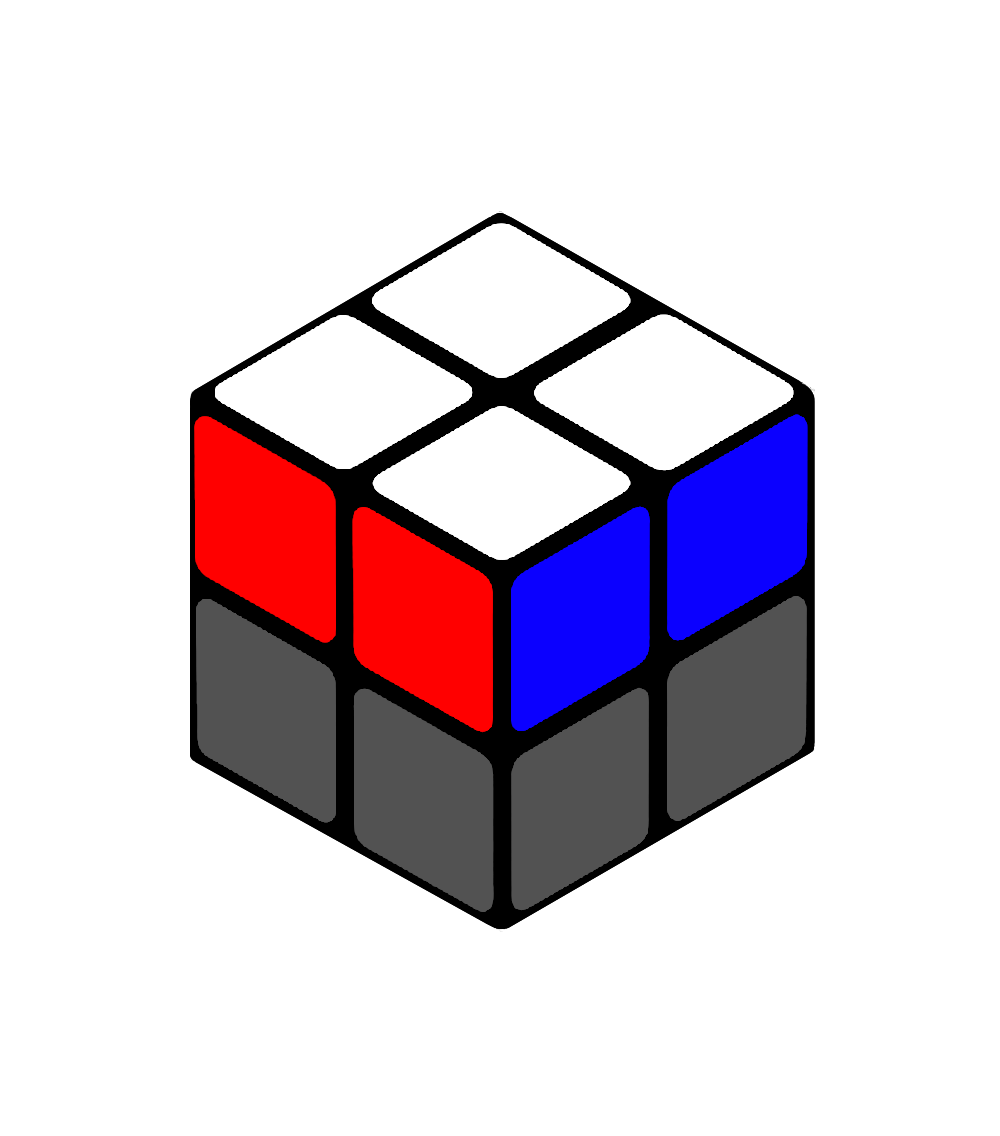
\includegraphics[scale=0.1]{ebene.png}
\caption[Ebene des Würfels]{Ebene des Würfels}
\label{Abbildung_Ebene}
\end{figure}

\begin{center}
\begin{tabular}{cl}
\toprule
\textbf{Abkürzung} & \textbf{Beschreibung des Zugs} \\
\midrule
$U$ & Drehung der \textbf{oberen} Ebene im Uhrzeigersinn \\
$D$ & Drehung der \textbf{unteren} Ebene im Uhrzeigersinn \\
$R$ & Drehung der \textbf{rechten} Ebene im Uhrzeigersinn \\
$L$ & Drehung der \textbf{linken} Ebene im Uhrzeigersinn \\
$F$ & Drehung der \textbf{vorderen} Ebene im Uhrzeigersinn \\
$B$ & Drehung der \textbf{hinteren} Ebene im Uhrzeigersinn \\
\bottomrule
\end{tabular} 
\end{center}

Die Kürzel stehen für \textit{Up, Down, Right, Left, Front, Back}. 
Die entsprechende Ebene wird um $90^\circ$ im Uhrzeigersinn gedreht, wenn auf diese Ebene geschaut wird. Dementsprechend wirkt es so, als würde die untere Ebene gegen den Uhrzeigersinn gedreht werden, wenn von oben auf den Würfel geschaut wird.  


Da der Würfel aber immer nur zwei nebeneinanderliegende Ebenen hat, entspricht eine Drehung der oberen Ebene nach rechts, einer Drehung der unteren Ebene nach links. 
Auf die Rotationsmöglichkeiten des kompletten Würfels wird im Verlauf dieser Arbeit noch eingegangen. Trotzdem werden die Drehungen für jede Ebene definiert. Das ist zwar nicht minimal, dient aber der besseren Anschaulichkeit und Übertragbarkeit der Algorithmen.
Sonst entspräche beispielsweise eine Drehung der oberen Ebene im Uhrzeigersinn ($U$) einer dreifachen Drehung der unteren Ebene im Uhrziegersinn ($DDD$) mit anschließender Rotation des kompletten Würfels. Es ist aber übersichtlicher, jede Ebenendrehung als einzelnen Zug darzustellen.



%
%
%
%
%
%
%
%
%=======================================================================================================
%
%
%
%
%
%
%
%
%


\newpage
\section{Mathematische Grundlagen}

\label{Kapitel_MathematischeGrundlagen}

In diesem Kapitel werden die mathematischen Grundlagen erklärt, die für den weiteren Inhalt dieser Arbeit relevant sind. Es werden Definitionen und Beispiele von Gruppen, Untergruppen, zyklischen Gruppen, Erzeugern, Gruppenoperationen, Kommutatoren, Äquivalenzrelationen, Permutationen und Zykelschreibweise angegeben.
Die genannten Definitionen basieren auf denen von Tobias Glosauer aus dem Buch \textit{Elementar(st)e Gruppentheorie} \cite{Buch}. Dort können auch detailliertere Informationen und weitere Beispiele nachlesen.
Des weiteren wird der Cayleygraph erklärt. 
%
%
%
%=======================================================================================================
%
%
%
\subsection*{Definition einer Gruppe} \addcontentsline{toc}{subsection}{\protect\numberline{}Definition einer Gruppe} \label{Abschnitt_Gruppe}


Die Definition einer Gruppe $(G, \circ)$ ist Grundlage für die folgenden Kapitel. 

\begin{definition}[Gruppe]
Eine Menge $G$ (auch Trägermenge) mit einer Verknüpfung $\circ$ wird Gruppe genannt, wenn diese Bedingungen gelten: 
\begin{itemize}
\item Abgeschlossenheit: $\forall a,b \in G.(a \circ b) \in G $
\item Assoziativität: $\forall a,b,c \in G.(a \circ b) \circ c = a \circ (b \circ c)$
\item Existenz eines neutralen Elements $n$: $\forall a \in G, \exists n \in G.n \circ a = a \circ n = a$ 
\item Existenz eines inversen Elements $a^{-1}$: $\forall a \in G, \exists a^{-1} \in G. a \circ a^{-1} = a^{-1} \circ a = n$ 
\end{itemize}
\end{definition}

Wenn es sich bei der Gruppe um eine kommutative Gruppe (auch abelsche Gruppe\footnote{\glqq Zu Ehren von Niels Henrik \textsc{Abel} (1802-1829); norwegischer Mathematiker und einer der Begründer der Gruppentheorie. Starb leider verarmt und deprimiert im Alter von 26 Jahren an Tuberkulose, kurz bevor er als Anerkennung für seine genialen Arbeiten  eine Dozentenstelle in Berlin angeboten bekam.\grqq \  \cite[S.21, Z.23]{Buch}}) handelt, muss zusätzlich noch die Eigenschaft der Kommutativität gelten: 

\begin{definition}[Kommutative Gruppe]
Eine Gruppe $(G, \circ)$ ist eine kommutative Gruppe, wenn gilt:
\begin{itemize}
\item Kommutativität: $\forall a,b \in G.(a \circ b) = (b \circ a) $
\end{itemize}
\end{definition}
\vspace*{0.1cm}


\begin{bsp}[Gruppe]

Zur Veranschaulichung der Gruppendefinition werden hier die natürlichen Zahlen $\mathbb{N}$ und die ganzen Zahlen $\mathbb{Z}$ mit dem Operator $+$ auf die Gruppenaxiome untersucht.
\begin{itemize}
\item Die Abgeschlossenheit gilt sowohl für $(\mathbb{N},+)$ als auch für $(\mathbb{Z},+)$, da zwei natürliche Zahlen addiert immer eine natürliche Zahl ergeben. Zwei ganze Zahlen addiert ergeben immer eine ganze Zahl. \\
Beispielsweise sind $1+2=3$ und es gilt $1,2,3 \in \mathbb{N}$.
\item Die Verknüpfung ist assoziativ, da das Pluszeichen so definiert ist.
\item Das neutrale Element von $(\mathbb{N},+)$ und $(\mathbb{Z},+)$ ist $0$. Es gilt also $\forall n \in N. \ n + 0 = 0 + n = n$ (und mit $\mathbb{Z}$ analog). \\
Ein Beispiel zur Veranschaulichung: $3+0=0+3=3$
\item Die letzte erfordleriche Eigenschaft einer Gruppe ist die Existenz eines inversen Elements. Für die Gruppe $(\mathbb{Z},+)$ ist $-z$ das inverse Element für jedes $z \in \mathbb{Z}$. Für $(\mathbb{N},+)$ gibt es kein inverses Element.
\end{itemize}
Anhand der oberen Axiome kann nun festgestellt werden, dass $(\mathbb{Z},+)$ die Gruppeneigenschaften erfüllt, $(\mathbb{N},+)$ aber nicht. 
$(\mathbb{Z},+)$ ist folglich eine Gruppe und $(\mathbb{N},+)$ nicht, da kein inverses Element existiert. 
Es ist aber zu beachten, dass es sich hierbei nicht um formelle Beweise, sondern um anschauliche Beschreibungen handelt.
Nun kann $(\mathbb{Z},+)$ noch auf die Kommutativität untersucht werden, um zu prüfen, ob es sich um eine abelsche Gruppe handelt. \\
Da der Plus-Operator als kommutativ definiert ist, ist $(\mathbb{Z},+)$ eine abelsche Gruppe.

\end{bsp}

\begin{bsp}[Gruppe]

Beispiele für endliche Gruppen sind die zyklischen Gruppen der Form $\mathbb{Z}_{\hspace*{-0.3em}\mod n}$. Hier wird die Menge für $n=6$ mit dem Additionsoperator auf die Gruppeneigenschaften untersucht. Die Elemente der Menge sind dann alle ganzen Zahlen modulo 6, also $\mathbb{Z}_{\hspace*{-0.3em}\mod 6}=\{0,1,2,3,4,5\}$
\begin{itemize}
\item Die Abgeschlossenheit gilt für $(\mathbb{Z}_{\hspace*{-0.3em}\mod 6}, +)$, da alle Elemente aus $\mathbb{Z}$ nach der Anwendung von $\mod 6$ in der Menge $\{0,1,2,3,4,5\}$ liegen.
\item Die Verknüpfung ist assoziativ, da das Pluszeichen so definiert ist.
\item Das neutrale Element von $(\mathbb{Z}_{\hspace*{-0.3em}\mod 6}, +)$ ist $0$.
\item Das Inverse Element für alle $z \in \mathbb{Z}_{\hspace*{-0.3em}\mod 6}$ ist definiert als $(6-z)$. Für 1 ist es demnach 5, für 2 ist es 4 und für 3 ist das neutrale Element die 3.
\end{itemize}

$(\mathbb{Z}_{\hspace*{-0.3em}\mod 6}, +)$ ist eine endliche Gruppe, da die vier Gruppeneigenschaften erfüllt sind und die Trägermenge $\mathbb{Z}_{\hspace*{-0.3em}\mod 6}$ endlich ist.

\end{bsp}

%
%
%
%
%
%=======================================================================================================
%
%
%
%
%
\subsection*{Untergruppen} \addcontentsline{toc}{subsection}{\protect\numberline{}Untergruppen} \label{Abschnitt_Untergruppe}

Im Folgenden werden Untergruppen definiert.


\begin{definition}[Untergruppe]
Eine Gruppe $(H, \circ)$ ist eine Untergruppe einer Gruppe $(G, \circ)$, wenn $H \subseteq G$ gilt. Dann wird auch $H \leqslant G$ geschrieben. 
\end{definition}

Das Symbol $\leqslant$ ist zu lesen als \textit{ist Untergruppe von}. Nicht jede Teilmenge $H \subseteq G$ muss auch eine Gruppe sein.

Wenn $(H, \circ)$ eine Untergruppe der Gruppe $(G, \circ)$ ist, wird $(G, \circ)$ auch Obergruppe von $(H, \circ)$ genannt.
Jede Gruppe G mit neutralem Element $N$ hat die beiden trivialen Untergruppen ${H_N = \{N\}}$ und $H_G=G$.


\begin{bsp}[keine Untergruppe]

Bei dem oben genannten Beispiel mit $(\mathbb{N},+)$ und $(\mathbb{Z},+)$ stellt sich heraus, dass $(\mathbb{Z},+)$ eine Gruppe ist und $(\mathbb{N},+)$ nicht. Obwohl $\mathbb{N \subseteq \mathbb{Z}}$, ist $(\mathbb{N},+)$ \textit{keine} Untergruppe von $(\mathbb{Z},+)$, da die Gruppeneigenschaft \textit{Existenz eines inversen Elements} nicht erfüllt sind.

\end{bsp}
\begin{bsp}[Untergruppe]

Es gilt $\mathbb{Z}_{\hspace*{-0.3em}\mod 6} \subseteq \mathbb{Z}$. Da sowohl $(\mathbb{Z},+)$, als auch $(\mathbb{Z}_{\hspace*{-0.3em}\mod 6}, +)$ Gruppen sind, ist $(\mathbb{Z}_{\hspace*{-0.3em}\mod 6}, +)$ eine Untergruppe von $(\mathbb{Z},+)$. $(\mathbb{Z}_{\hspace*{-0.3em}\mod 6}, +)$ und $(\mathbb{Z},+)$ wurden im Abschnitt über Gruppen auf die Gruppeneigenschaften untersucht.

\end{bsp}

%
%
%
%
%
%=======================================================================================================
%
%
%
%
%

\subsection*{Erzeuger und zyklische Gruppe} \addcontentsline{toc}{subsection}{\protect\numberline{}Erzeuger und zyklische Gruppe}



\begin{definition}[Erzeuger]
Sei die Menge $M \subseteq G$ eine nicht leere Teilmenge der Trägermenge einer Gruppe $(G, \circ)$. 
Dann wird die Untergruppe $(M, \circ)$ von $M$ erzeugt und ist die kleinste Untergruppe von $(G, \circ)$, für die $M \subseteq G$ gilt.
$(M, \circ)$ wird dann Erzeugnis von $M$ genannt und die Elemente aus $M$ sind die Erzeuger der Untergruppe $(M, \circ)$.
\end{definition}

Wenn $(M, \circ)$ durch $M$ erzeugt wird, ist dann eine $M$ enthaltende Untergruppe.

Eine zyklische Gruppe ist eine Gruppe, die von nur einem Element erzeugt wird. Sie besteht nur aus Potenzen dieses Elementes

\begin{definition}[Zyklische Gruppe]
Sei $(G, \circ)$ eine Gruppe. $(G, \circ)$ wird zyklische Gruppe genannt, wenn es ein Element $a \in G$ gibt, das jedes Element in $G$ erzeugt. Dann schreibt man auch:
\begin{align*}
\langle a \rangle := \{ a^n \mid n \in \mathbb{Z} \}
\end{align*}

\end{definition}


\begin{bsp}[Erzeuger und zyklische Gruppe]

Ein Beispiel für Erzeuger findet sich anhand der Gruppe der ganzen Zahlen $(\mathbb{Z},+)$ und der Addition als Verknüpfung, die bereits als Beispiel der Gruppe beschrieben wurde.

Die Operationen sind hier die Addition und der Übergang von einer Zahl $z$ zu der negativen Zahl $-z$.

Ein Erzeuger dieser Gruppe ist die einelementige Menge $M = \{ 1 \}$. Jede positive Zahl $n$ lässt sich durch die $n$-fache Addition von $1$ erzeugen und jede negative Zahl durch  die Addition von $((-1)+(-1)...)$. 

\end{bsp}
%
%
%
%
%=======================================================================================================
%
%
%
%
%
\subsection*{Cayleygraph} \addcontentsline{toc}{subsection}{\protect\numberline{}Cayleygraph}\label{Abschnitt_Cayleygraph}
Ein Cayleygraph ist ein Graph, der die Struktur einer Gruppe beschreibt. Er hängt von der Menge der Erzeuger ab und dient dazu, Gruppen bildlich darzustellen.
Es handelt sich dabei um einen Graphen mit Knoten, die die verschiedenen Gruppenelemente darstellen. Pfeile zeigen von einem Element zum nächsten, wenn dies durch einen der Erzeuger erreicht werden kann. \cite{AT}

\textbf{Beispiel} (Cayleygraph) \\
In Abbildung \ref{Abbildung_Cayleygraph} ist den Cayleygraphen der Gruppe $(\mathbb{Z}_{\hspace*{-0.3em}\mod 6}, +)$ mit dem Erzeuger $1$ zu sehen.

\begin{figure}[H]
\centering
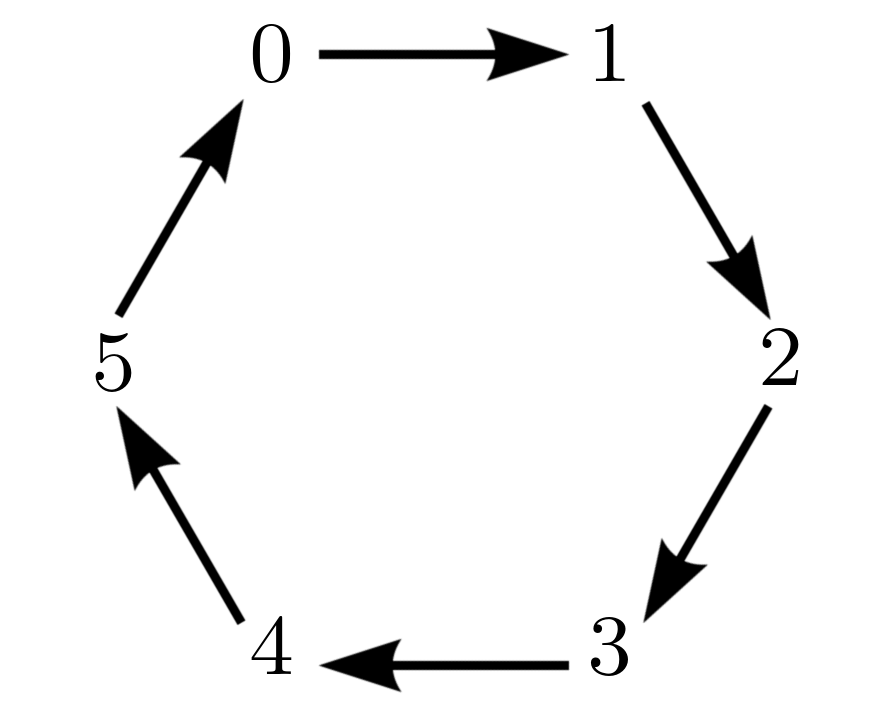
\includegraphics[scale=0.7]{Cayleygraph3.png}
\caption{Cayleygraph von $(\mathbb{Z}/6\mathbb{Z}, +)$ mit Erzeuger $1$}
\label{Abbildung_Cayleygraph}
\end{figure}


%
%
%
%
%=======================================================================================================
%
%
%
%
%
%

\subsection*{Gruppenoperation} \addcontentsline{toc}{subsection}{\protect\numberline{}Gruppenoperation} \label{Abschnitt_Gruppenoperation}



Es gibt Links- und Rechtsoperationen auf Gruppen. Da in dieser Arbeit nur Rechtsoperationen genutzt werden, beschränkt sich die Definition darauf.


\begin{definition}[Rechtsoperation]

Eine Rechtsoperation einer Gruppe $(G, \circ)$ auf einer Menge $M$ ist eine Verknüpfung mit $m \in M$, $e$ als neutralem Element von $(G,\circ)$ und $g,h \in G$:
\begin{align*}
\cdot: M \times G \rightarrow M \ \ \ \ \ \ \ \ \ \ \ \ \ \ \
(m, g) \mapsto m \cdot g 
\end{align*}
Die folgenden beiden Eigenschaften gelten:
\begin{align*}
m \cdot e & = m \\
m \cdot (g \circ h) & = (m \cdot g) \cdot h
\end{align*}
Dann operiert $G$ von rechts auf $M$.

\end{definition}


\begin{bsp}[Rechtsoperation]

Als Beispiel werden die Gruppe $(\mathbb{Z}_{\hspace*{-0.3em}\mod 6}, +)$ und die Menge $\mathbb{Z}$ mit der Verknüpfung $-$ betrachtet. Die folgenden Eigenschaften gelten, da $(\mathbb{Z}_{\hspace*{-0.3em}\mod 6}, +)$ eine Rechtsoperation auf $\mathbb{Z}$ ist, mit $z \in  \mathbb{Z}$ und $g,h \in \mathbb{Z}_{\hspace*{-0.3em}\mod 6}$.
\begin{itemize}
\item Die Eigenschaft $z - 0 = z$ ist erfüllt. $0$ ist das neutrale Element von $(\mathbb{Z}_{\hspace*{-0.3em}\mod 6}, +)$.
\item Da sich $z-(g+h)$ zu $z-g-h$ umformen lässt, gilt $z-(g+h) = (z-g)-h$
\end{itemize}
Demnach operiert $(\mathbb{Z}_{\hspace*{-0.3em}\mod 6}, +)$ mit $-$ von rechts auf $\mathbb{Z}$.

\end{bsp}

%
%
%
%
%
%=======================================================================================================
%
%
%
%
%
%
%

\subsection*{Kommutator} \addcontentsline{toc}{subsection}{\protect\numberline{}Kommutator
} \label{Abschnitt_Kommutator}
Die Komplexität eines Kommutators sagt etwas darüber aus, wie sehr zwei Elemente einer Gruppe das Kommutativgesetz verletzen. Bei kommutativen Gruppen ist der Kommutator zweier Elemente das neutrale Element der Gruppe \cite{TD}. Man sagt dann, dass die beiden Elemente kommutieren. 


\begin{definition}[Kommutator]
Als Kommutator von zwei Elementen $a, b$ einer Gruppe $(G, \circ)$  bezeichnet man $[a,b] = aba^{-1}b^{-1}$.
\end{definition}


\begin{bsp}[Kommutator]

$[5,7]$ ist ein Kommutator der Gruppe $(\mathbb{Z}, +)$. $[5,7]$ ist das Gleiche wie $5+7-5-7 = 0$ und $0$ ist das neutrale Element der Gruppe. Die Gruppe $(\mathbb{Z}, +)$ ist kommutativ, deshalb ist der Kommutator von allen Elementen der Gruppe $0$.

\end{bsp}
%
%
%
%
%
%
%=======================================================================================================
%
%
%
%
%
%
%

\subsection*{Äquivalenzrelation} \addcontentsline{toc}{subsection}{\protect\numberline{}Äquivalenzrelation} \label{Abschnitt_Äquivalenrelationen}

Mit Relationen lassen sich Beziehungen von Elementen einer Menge zueinander beschreiben.

\begin{definition}[Äquivalenzrelation]
Eine Relation $\sim \ \subseteq A \times A$ heißt Äquivalenzrelation auf $A$, wenn für alle $x, y, z \in A$ die drei folgenden Eigenschaften gelten: Reflexivität, Symmetrie, Transitivität.
\end{definition}


Hier wird $x \sim y$ als \textit{x ist äquivalent zu y} gelesen. Im Folgenden werden noch die Bedeutungen von Reflexivität, Symmetrie und Transitivität aufgelistet:

\begin{center}
\begin{tabular}{ll}
$x \sim x$ & (Reflexivität) \\
Aus $(x \sim y)$ folgt $(y \sim x)$. & (Symmetrie) \\
Aus $(x \sim y)$ und $(y \sim z)$ folgt $(x \sim y)$. & (Transitivität) \\
\end{tabular}
\end{center}


\begin{bsp}[Relation]


Für die Menge $A=\{ 1, 2, 3, 4, 5 \}$ wird die Relation $ x < y$ betrachtet:

Bei der Relation $< $ handelt es sich nicht um eine Äquivalenrelation, da die Eigenschaft der Reflexivität nicht gilt: $1 \nless 1$. Auch die Symmetrie gilt nicht.


\end{bsp}
\begin{bsp}[Äquivalenzrelation]
Für die Menge $A=\{ 1, 2, 3, 4, 5 \}$ wird die Relation $ x = y$ betrachtet:

Bei der Relation $=$ gilt die Reflexivität für alle Elemente, da die Gleichheit reflexiv ist. Auch die Symmetrie und die Transitivität gelten für die Gleichheit. Somit ist es eine Äquivalenzrelation. 


\end{bsp}

\begin{bsp}[Äquivalenzrelation]
Für die Menge $A=\{ -3, -2, -1, 0, 1, 2, 3 \}$ wird die Relation $x \sim_+ y$ betrachtet, die als $|x| =|y|$ definiert ist:

Bei der Relation $\sim_+$ gilt die Reflexivität für alle Elemente, da die Gleichheit reflexiv ist. Auch die Symmetrie und die Transitivität gelten für die Gleichheit mit Betrag. Somit ist es eine Äquivalenzrelation. 


\end{bsp}
%
%
%
%
%
%
%=======================================================================================================
%
%
%
%
%
%
%
\subsection*{Äquivalenzklassen und Faktormenge} \addcontentsline{toc}{subsection}{\protect\numberline{}Äquivalenzklassen und Faktormenge}
\label{Abschnitt_FaktormengenUndÄquivalenzklasse}

Äquivalenzklassen sind Mengen, die äquivalente Elemente enthalten.

\begin{definition}[Äquivalenzklassen]

Sei $ \sim $ eine Äquivalenzrelation auf der Menge $M$ und $x \in M$. Die Äquivalenzklasse von $x$ wird dann als $[x]$ geschrieben und ist definiert als $\{y \in M \mid y \sim x\} \subseteq M$.  

\end{definition}

Jedes Element der Äquivalenzklasse $[x]$ heißt \textit{Repräsentant von $[x]$}. Alle Repräsentanten von $[x]$ sind äquivalent zu $x$.

\begin{bsp}[Äquivalenzklassen]
Es wird die Äquivalenzrelation $x \sim_+ y$, die als $|x| =|y|$ definiert ist, auf der Menge $A=\{ -3, -2, -1, 0, 1, 2, 3 \}$ betrachtet. Die Äquivalenzklasse von $[1]$ beispielsweise ist dann $[1] = \{x \in A \mid x \sim_+ 1\}$. $[1]$ enthält dann die Elemente $1$ und $-1$.

\end{bsp}

\begin{definition}[Faktormenge]

Die Faktormenge $M / \sim $ der Menge $M$ bezüglich der Äquivalentionrelation $\sim$ besteht aus allen Äquivalentzklassen und ist definiert als $\{ [x] \mid x \in M \}$.

\end{definition}

$M / \sim $ wird als \textit{$M$ modulo $\sim$} gelesen. Die Elemente von $M / \sim $ sind Äquivalenzklassen.

\begin{bsp}[Faktormenge]

Es wird wieder die Äquivalenzrelation $x \sim_+ y$, die als $|x| =|y|$ definiert ist, auf der Menge $A=\{ -3, -2, -1, 0, 1, 2, 3 \}$ betrachtet.  \\
Die Faktormenge $A / \sim_+$ enthält dann die Äquivalenzklassen $[1]$, $[2]$, $[3]$ und $[0]$. $A / \sim_+$ also vier Elemente, während $A$ sieben Elemente hat.

\end{bsp}

%
%
%
%
%
%
%=======================================================================================================
%
%
%
%
%
%
%
\subsection*{Mächtigkeit einer Gruppe} \addcontentsline{toc}{subsection}{\protect\numberline{}Mächtigkeit einer Gruppe}
\label{Abschnitt_MächtigkeitGruppe}

Die Mächtigkeit einer Gruppe $(G, \circ)$ wird auch Gruppenordnung genannt und sagt aus, wie viele Elemente die Menge $G$ der Gruppe enthält.

\begin{definition}[Mächtigkeit einer Gruppe]
Die Mächtigkeit einer Gruppe $(G, \circ)$ ist der Betrag der Menge $G$, also $|G|$. 
\end{definition}

Wenn $|G| < \infty$, wird von einer endlichen Gruppe gesprochen.

\begin{bsp}[Mächtigkeit einer endlichen Gruppe]

Die Mächtigkeit der Gruppe $(\mathbb{Z}_{\hspace*{-0.3em}\mod 6}, +)$ ist $6$. Die Menge $\mathbb{Z}_{\hspace*{-0.3em}\mod 6}$ enthält die Elemente $\{0,1,2,3,4,5 \}$ und somit ist $| \mathbb{Z}_{\hspace*{-0.3em}\mod 6} | = 6$.

\end{bsp}

\begin{bsp}[Mächtigkeit einer unendlichen Gruppe]

Die Mächtigkeit der Gruppe $(\mathbb{Z}, +)$ ist $\infty$, da $|\mathbb{Z}|$ (abzählbar) unendlich ist.

\end{bsp}
%
%
%
%
%
%
%=======================================================================================================
%
%
%
%
%
%
%
\subsection*{Permutationen und Zykelschreibweise} \addcontentsline{toc}{subsection}{\protect\numberline{}Permutationen und Zykelschreibweise} \label{Abschnitt_PermutationZykel}

Unter einer Permutation versteht man die Reihenfolge von Objekte.

\begin{definition}[Permutation]
Bei einer $n$-elementigen Menge $M$ ist eine ($n$-stellige) Permutation ist eine bijektive Abbildung $\pi  : M \rightarrow M$.
\end{definition}
Die Zykelschreibweise ist eine kurze Schreibweise für eine Permutation.
Die Zykelschreibweise wird nun anhand eines Beispiels erklärt. Die Definition geht über den Rahmen dieser Arbeit hinaus, sie kann aber in dem Buch \textit{Elementar(st)e Gruppentheorie} von Tobias Glosauer \cite{Buch} nachgelesen werden.

\begin{bsp}[Permutationen und Zykelschreibweise]
Sei $M$ eine Menge mit fünf Objekten: $1, 2, 3, 4$ und $5$. Nun können diese Objekte in fünf Plätzen arrangiert werden. Die Plätze werden als $1$ bis $5$ nummeriert. Dann kann eine Funktion $\pi :\{1,2,3,4,5\} \rightarrow \{1,2,3,4,5\}$ definiert werden, bei der $\pi (i)$ die Zahl ist, die in Slot $i$ liegt.
Wenn die Zahlen in der Reihenfolge $5 \ 1\ 4\ 3 \ 2$ amgeordnet werden, ist $5$ auf Platz $1$, $1$ auf Platz $2$, usw. Das ist auch in der folgenden Tabelle zu sehen: 

\begin{center}
\begin{tabular}{l ccccc}

Platz & 1 & 2 & 3 & 4 & 5 \\
\midrule
Zahl & 5 & 1 & 4 & 3 & 2 \\

\end{tabular}
\end{center}

Die Funktion $\pi$ sieht für diese Permutation (s. Tabelle) so aus:
\begin{align*}
\pi(1) = 5 \ \ \ \ \ \  \pi(2) = 1 \ \ \ \ \ \ \pi(3) = 4 \ \ \ \ \ \ \pi(4) = 3 \ \ \ \ \ \ \pi(5) = 2 
\end{align*}
$\pi$ kann auch als eindeutige Zuordnung der Form $i \mapsto j$ (für $\pi(i)=j$) geschrieben werden \cite{JC}:
\begin{align*}
1 \mapsto 5 \ \ \ \ \ \ \ \ \ \  2\mapsto 1 \ \ \ \ \ \ \ \ \ \ 3\mapsto 4 \ \ \ \ \ \ \ \ \ \ 4\mapsto 3 \ \ \ \ \ \ \ \ \ \ 5\mapsto 2 
\end{align*}
Das kann auch in der Zykelschreibweise geschrieben werden:
\begin{align*}
\pi = (1 \ 5 \ 2)\ (3 \ 4)
\end{align*}
Das wird so gelesen: Die 1 geht auf die 5, die 5 geht auf die 2, die 2 geht wieder auf die 1. Damit ist der erste Zykel geschlossen. Beim zweiten Zykel geht die 3 auf die 4 und die 4 auf die 3. $\pi$ besteht somit aus zwei Zykeln: ein Zykel hat die Länge drei und der andere die Länge zwei. Die Zykel sind auch in Abbildung \ref{Abbildung_ZykelVonf} zu sehen.
\begin{figure}[H]
\centering
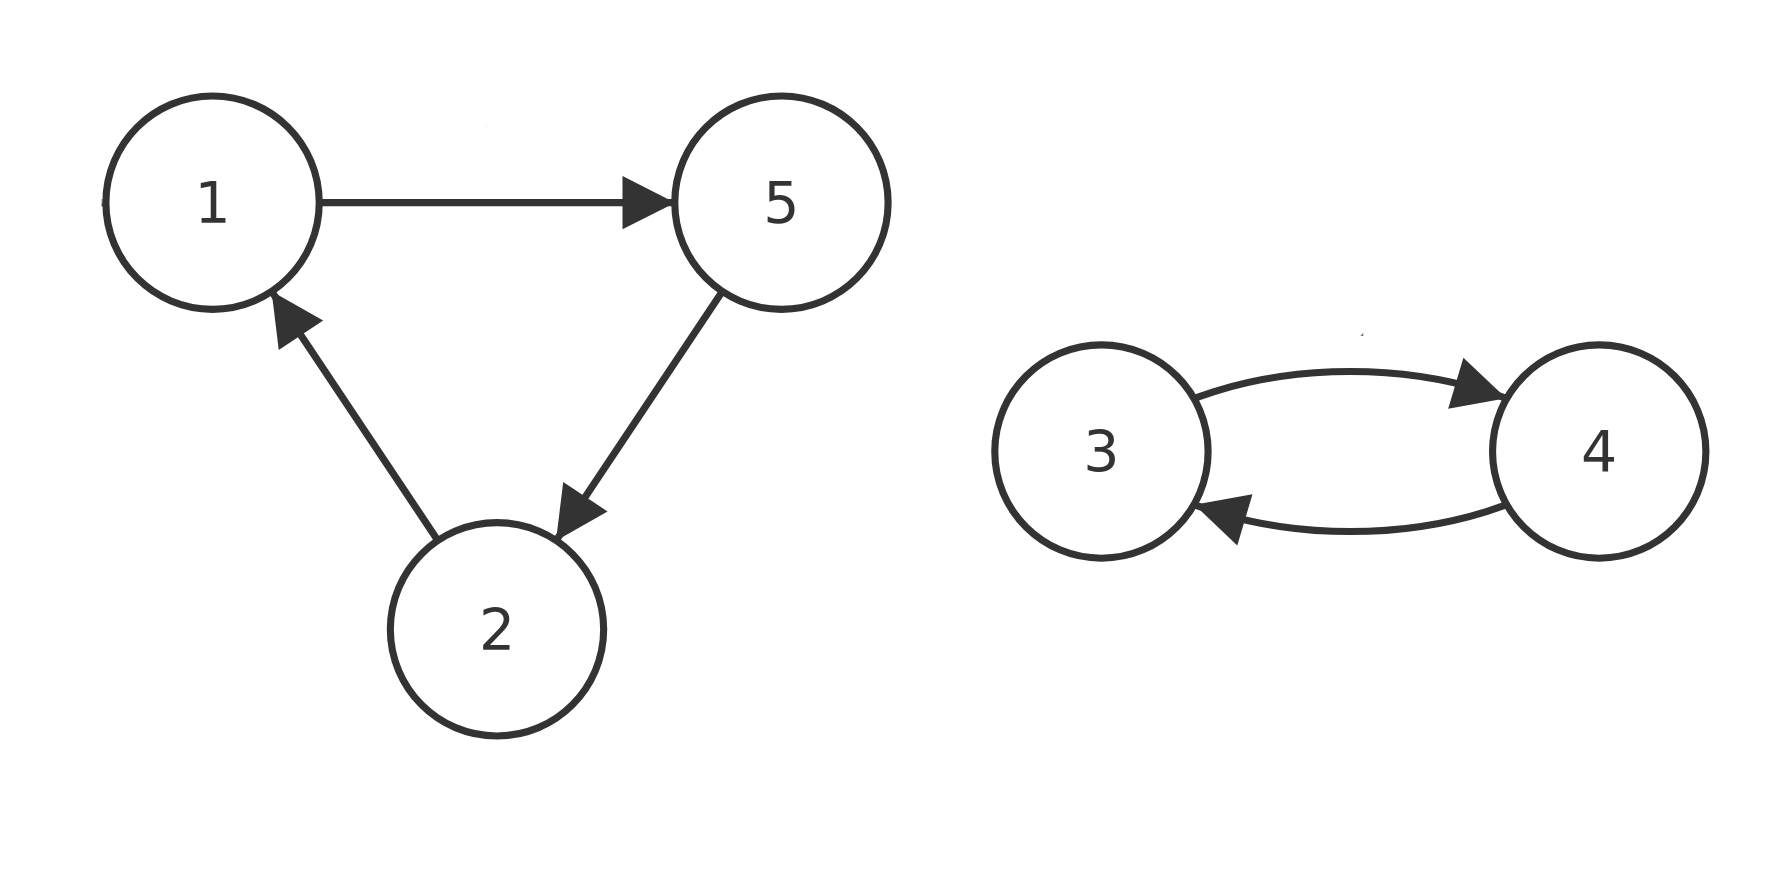
\includegraphics[scale=0.13]{Zykel_152.png}
\caption{Zykel $\pi = (1 \ 5 \ 2)\ (3 \ 4)$}
\label{Abbildung_ZykelVonf}
\end{figure}
Bei der Zykelschreibweise ist die Reihenfolge der Elemente wichtig. Beispielsweise ist $(1 \ 2 \ 3)$ nicht das gleiche wie $(1 \ 3 \ 2)$. Wenn die Reihenfolge bestehen bleibt, können die Zykel aber bei jedem beliebigen Element beginnen. Das Beispiel $(1 \ 2 \ 3)$ kann demnach auch als $(2 \ 3 \ 1)$ oder $(3\ 1 \ 2 \ )$ geschrieben werden.

Die Identitätspermutation wird als $\pi = 1$ geschrieben. Dabei werden alle Elemente auf sich selbst abgebildet und die Zykel bleiben somit unverändert.
\end{bsp}

\begin{definition}[Anzahl der Permutationen]
Für $n$ verschiedene Objekte ist die Anzahl der Permutationen $n!$.
\end{definition}

\begin{bsp}[Anzahl der Permutationen]
Sei $\pi = (1 \ 2 \ 3)$ eine Permutation mit 3 Objekten. Für das erste Objekt der Permutation gibt es $3$ Möglichkeiten: $1$, $2$ oder $3$. Für das zweite Objekte dann nur noch $2$ Möglichkeiten (da eine ja bereits im ersten Schritt eliminiert wurde) und danach nur eine. Es gibt dann also $3 \cdot 2 \cdot 1 = 3! = 6$ Möglichkeiten.

\end{bsp}
%
%
%
%
%
%
%=======================================================================================================
%
%
%
%
%
%
%

\newpage
\subsection*{Parität} \addcontentsline{toc}{subsection}{\protect\numberline{}Parität}
\label{Abschnitt_GrundlagenParität}

\begin{definition}[Parität]
Eine Zahl $n \in \mathbb{Z}$ ist gerade, wenn sie ganzzahlig ohne Rest durch zwei teilbar ist. Ansonsten ist sie ungerade. Die Menge der ganzen Zahlen wir dadurch in zwei Teilmengen zerlegt. Das nennt man Parität.
\end{definition}

Ungerade Zahlen ergeben bei der Division durch $2$ immer einen rest von $1$. Gerade Zahlen haben dabei den Rest $0$.

\begin{bsp}[Parität]

Sei $M=\{-2, -1, 0, 1, 2\}$. Die Teilmenge $\{-2, 0, 2\}$ enthält nur gerade Elemente und die Teilmenge $\{ -1, 1\}$ nur ungerade Elemente.

\end{bsp}

%
%
%
%
%=======================================================================================================
%
%
%
%
%
%\subsection*{Symmetrische Gruppe} \addcontentsline{toc}{subsection}{\protect\numberline{}Symmetrische Gruppe}\label{Abschnitt_SymmetrischeGruppe}

%\begin{definition}[Symmetrische Gruppe]
%Eine Gruppe $(S, \circ)$ ist symmetrisch, wenn $S$ aus allen Permutationen (s. Kapitel \ref{Abschnitt_PermutationZykel}) einer Menge besteht. 
%\end{definition}

%\begin{bsp}
%Die Gruppe $(S, \circ)$ mit $S = \{(a \ b),(b \ a),(a \ c),(c \ a),(b \ c),(c \ b)\}$ ist eine symmetrische Gruppe, die aus allen Permutationen der Elemente $a, b$ und $c$ besteht. Der $\circ$-Operator verknüpft zwei Permutationen. Werden beispielsweise $(a \ b)$ und $(b \ c)$ verknüpft, so gilt dann $(a \ b)\circ (b \ c) = (a \ c)$, was auch in $S$ enthalten ist. (Das inverse Element ist der jeweilige Zykel \textit{rückwärts}, das neutrale Element sind die einelementigen Zykel $(a)(b)(c)$, die durch Verknüpfung eines Zykels mit seinem Inversen entstehen.)
%\end{bsp}

%\begin{definition}[Mächtigkeit einer symmetrischen Gruppe]
%Eine symmetrische Gruppe $(S, \circ)$, die aus allen Permutationen einer $n$-elementigen Menge $M$ besteht, hat die Mächtigkeit $n!$.
%\end{definition}

%\begin{bsp}[Mächtigkeit einer symmetrischen Gruppe]
%Bei der symmetrischen Gruppe $(S, \circ)$ mit $S = \{(a \ b),(b \ a),(a \ c),(c \ a),(b \ c),(c \ b)\}$ enthält $S$ die Permutationen aller Elemente der $3$-elementigen Menge $\{a, b, c\}$. Somit ist die Mächtigkeit der Gruppe $3! = 1 \cdot 2 \cdot 3 = 6 \ ( \ = |S|\ )$. 
%\end{bsp}
%
%
%
%
%=======================================================================================================
%
%
%
%
%
%
\newpage

\section{Konfiguration des Würfels}

\label{Kapitel_KonfigurationDesWürfels}

Um mit dem Würfel zu arbeiten, muss festgestellt werden, in welcher Position er sich befindet.
Deshalb wird die Konfiguration des Würfels definiert, bevor der Würfel als Gruppe dargestellt wird. Eine Würfelkonfiguration setzt sich aus zwei Parametern zusammen: 
\begin{itemize}
\item Position der Ecksteine (angegeben als $\sigma$)
\item Ausrichtung der Ecksteine (angegeben als $x$)
\end{itemize}
Die Konfiguration des Würfels kann als 2-Tupel geschrieben werden: $(\sigma, x)$.
In diesem Kapitel wird die Position der Ecksteine als $\sigma$ und die Ausrichtung der Ecktsteine als Vektor $x$ erklärt. 

%
%
%
%
%
%
%
%
%
%
%=======================================================================================================
%
%
%
%
%
%
%
%
%
%

\subsection*{Positionen der Steine im Würfel} \addcontentsline{toc}{subsection}{\protect\numberline{}Positionen der Steine im Würfel}

Die Menge der bijektiven Funktionen $\sigma$ (für jede Ebenenrotation) stellt Übergänge der Würfelsteine als Funktion dar. Die Übergänge beschreiben die Positionsänderung der Steine bei einem Zug. $\sigma$ bildet jede der Würfelpositionen auf die neue Position ab. Es handelt sich dabei um eine Permutation. Permutationen wurden in Kapitel \ref{Abschnitt_PermutationZykel} erklärt. 

Die Einteilung der Würfelpositionen sind in den Abbildungen \ref{Abbildung_SteinpositionNamen} und \ref{Abbildung_SteinpositionNamenFoldetOut} zu sehen. Die einzelnen Steinpositionen werden mit den Kürzeln benannt, die \textit{up, down, right, left, front und back} beschreiben.
\begin{figure}[h]
\centering
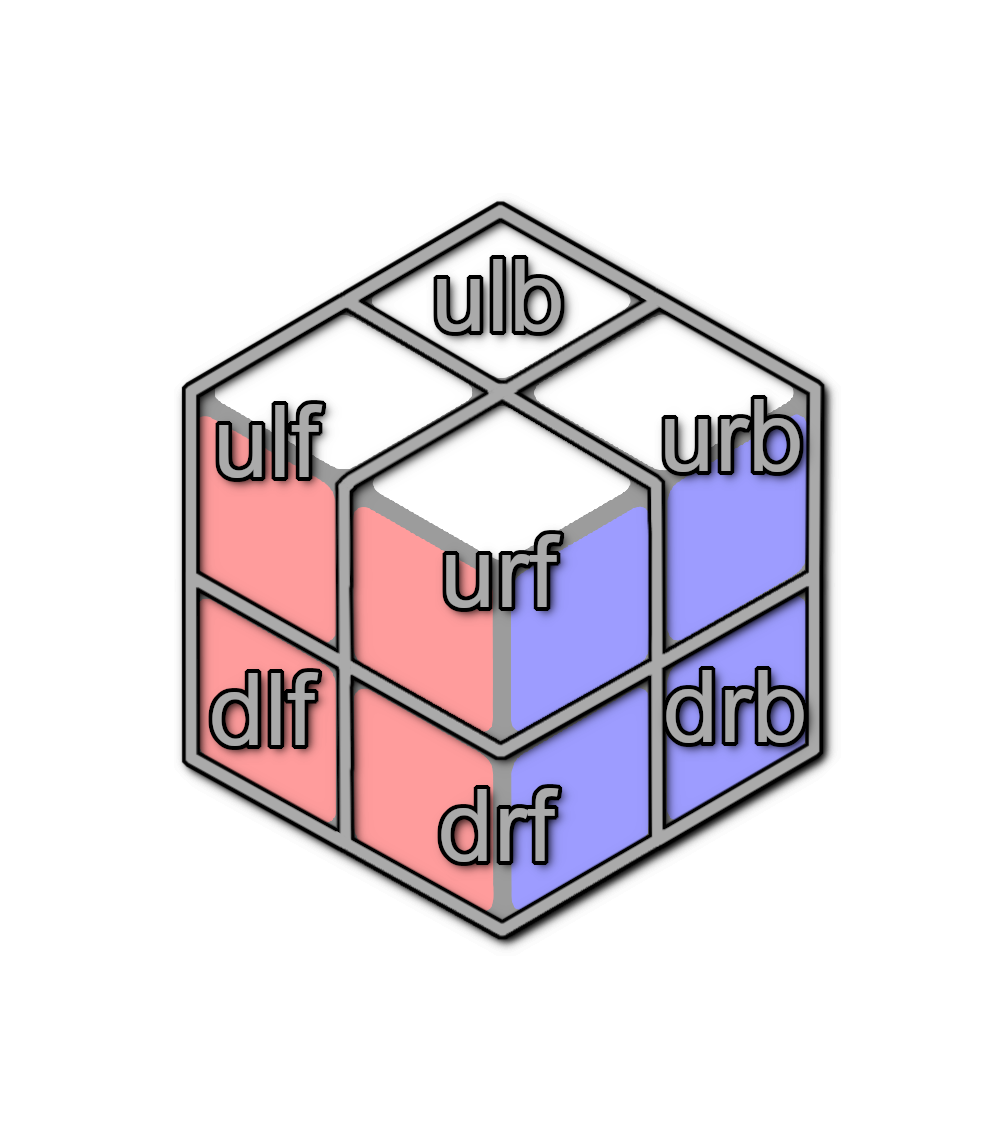
\includegraphics[scale=0.15]{caged_positions.png} \\
\caption[Namen der Steinpositionen im Würfel]{Namen der Steinpositionen im Würfel}
\label{Abbildung_SteinpositionNamen}
\end{figure}

\begin{figure}[h]
\centering
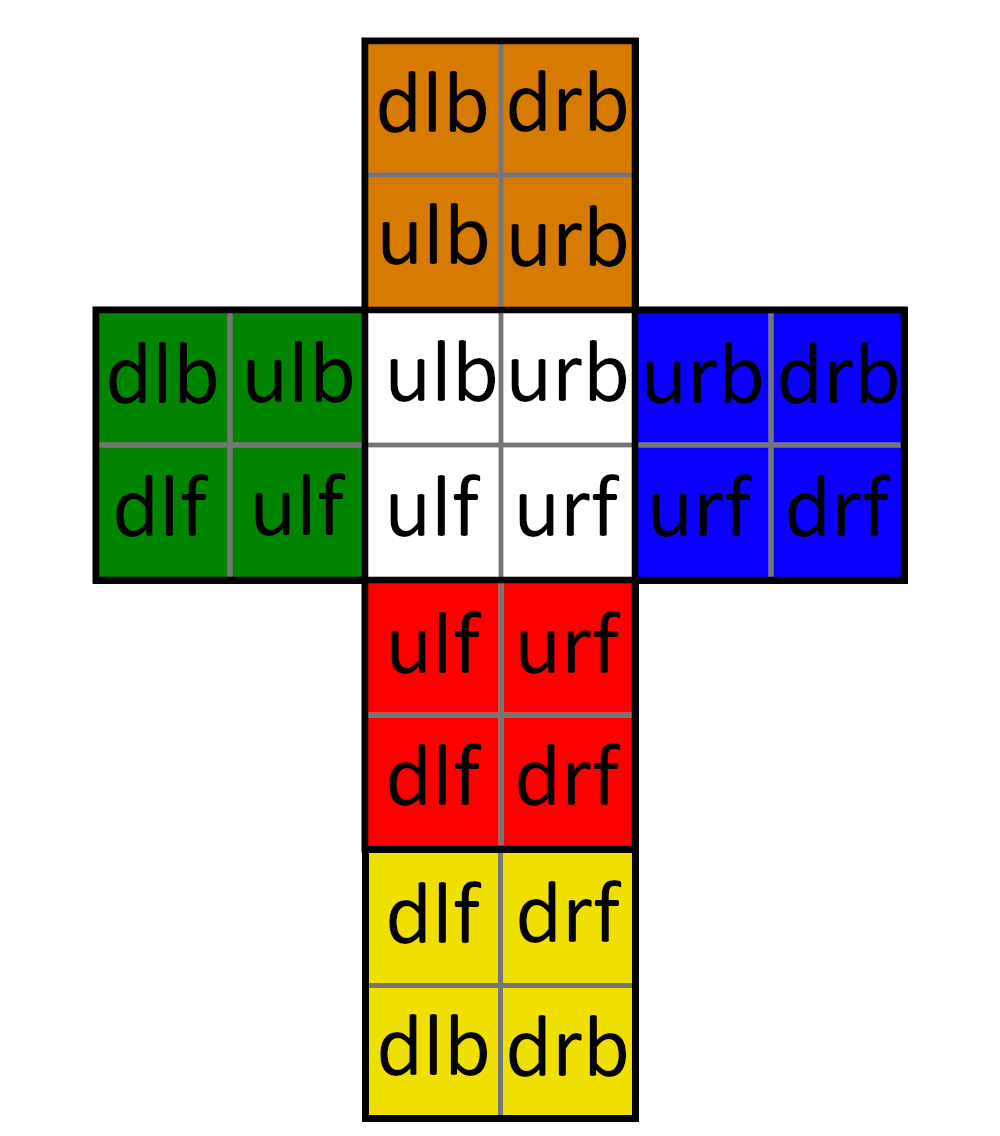
\includegraphics[scale=0.15]{foldedout_cage.png}
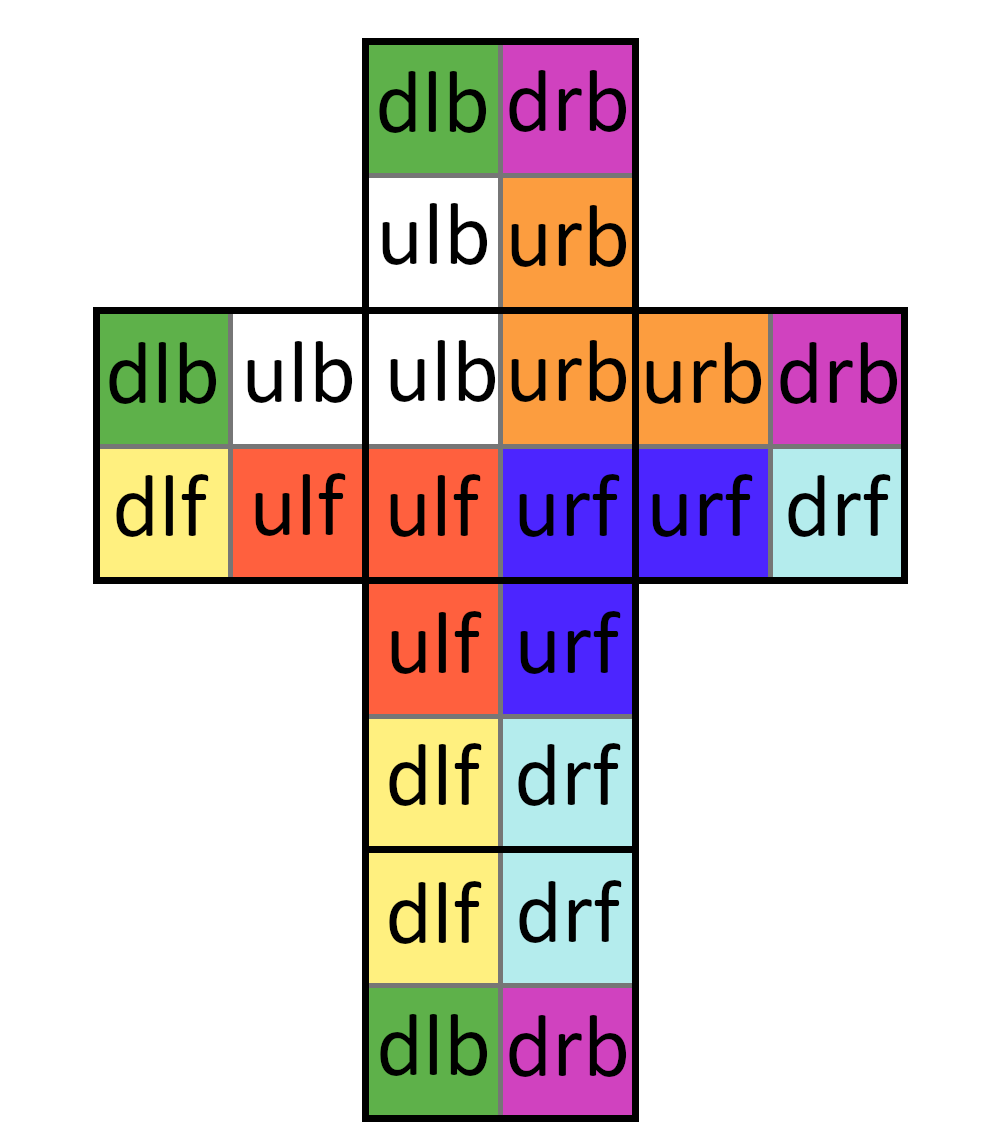
\includegraphics[scale=0.15]{foldedout_cage_color.png}
\caption[aufgeklappter Würfel mit Namen der Steinpositionen]{aufgeklappter Würfel mit Namen der Steinpositionen}
\label{Abbildung_SteinpositionNamenFoldetOut}
\end{figure}
Jeder Steinposition wird ein einzigartiger Name zugeordnet, um sich darauf zu beziehen. Dabei wird davon ausgegangen, dass die weiße Seite in der Startkonfiguration oben ist und die rote Seite vorne. Die Steinposition werden mit 3 Buchstaben beschrieben, die aus den Kürzeln \textit{u, d, r, l, f, b} bestehen. Diese Kürzel stehen für \textit{up, down, right, left, front, back}. \\
Somit heißt die Steinposition oben links beispielsweise \textit{ulf} (für \textit{up}, \textit{left} und \textit{front}). 
Jeder Stein bekommt auch einen eindeutigen Namen, der seiner Steinposition im gelösten Zustand entspricht. Beispielsweise liegt der Stein \textit{ulf} im gelösten Zustand an der Steinposition \textit{ulf}.

Nun wird zur Veranschaulichung die Permutation $\sigma_U$ für eine Drehung der oberen Ebene um 90$^\circ$ im Uhrzeigersinn definiert. Grundlagen zu Permutationen und der Zykelschreibeweise wurden in Kapitel \ref{Abschnitt_PermutationZykel} erklärt.
Hier wird $\sigma_U$ ausführlich beschrieben und verschiedene Schreibweisen angegeben. Die weiteren Drehungen sind analog definiert. 
Die Drehung der oberen Ebene ist in Abbildung \ref{Abbildung_SteinpositionnamenNachU} grafisch dargestellt.
\begin{figure}[h]
\centering
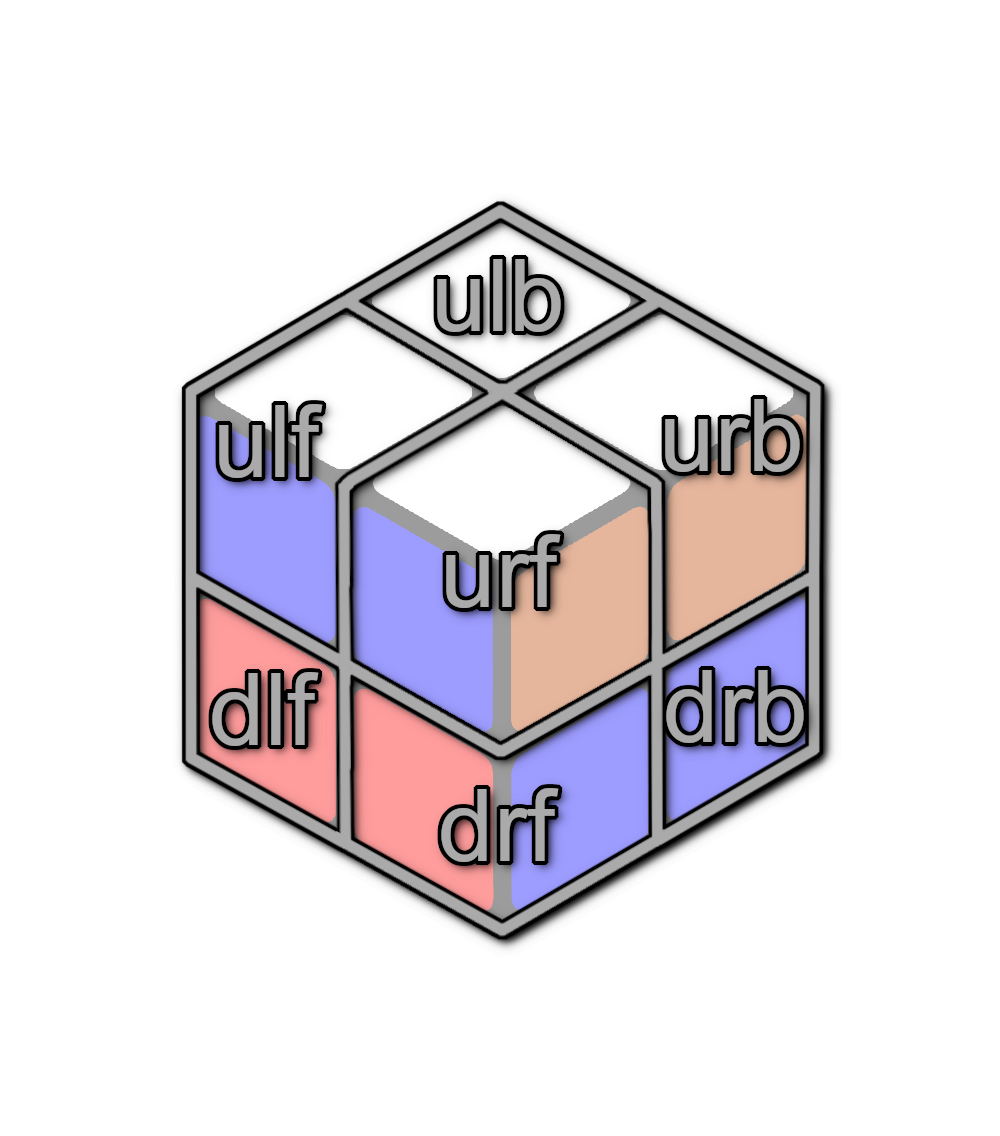
\includegraphics[scale=0.13]{caged_spin.png}
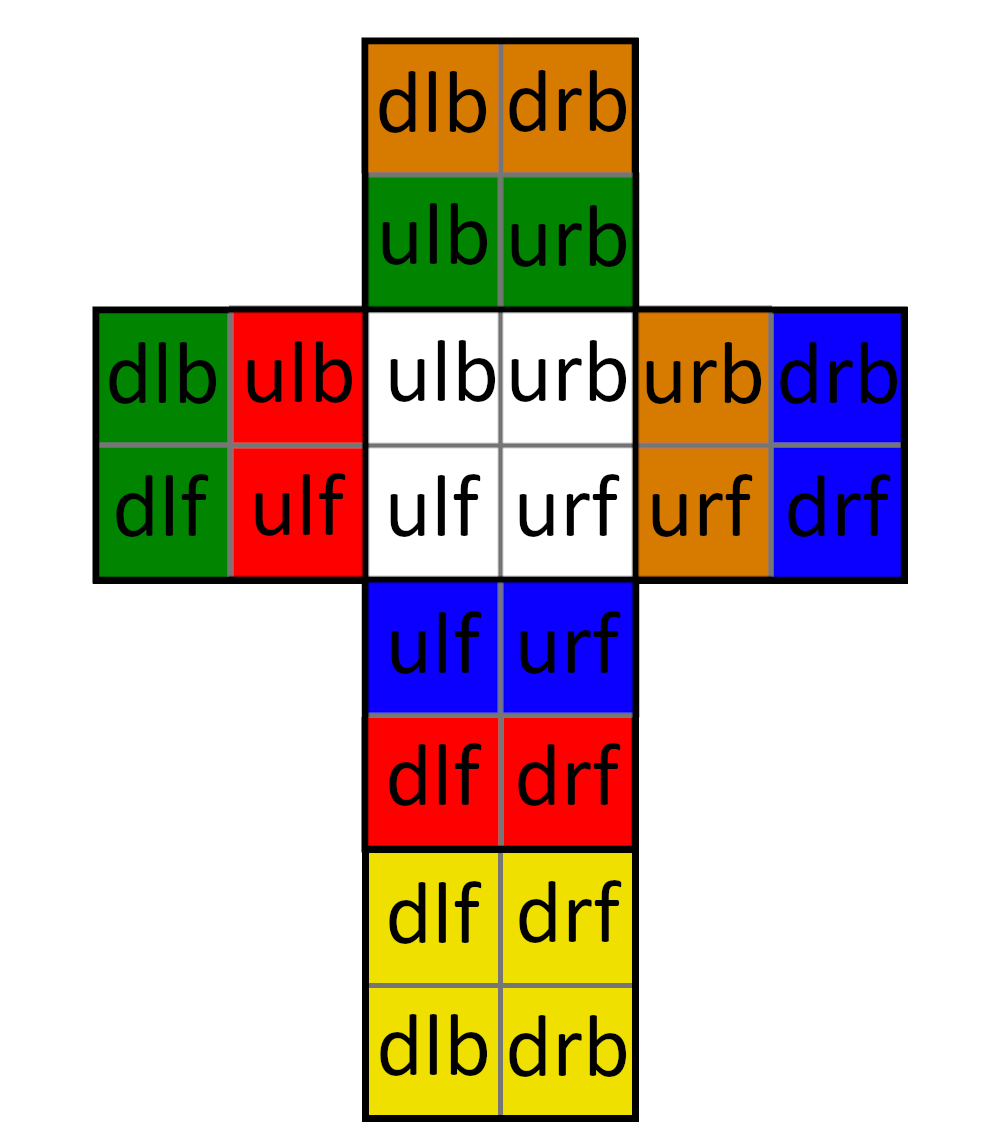
\includegraphics[scale=0.13]{foldedout_spin.png}
\caption[Steinpositionen nach Zug $U$]{Steinpositionen nach Zug $U$}
\label{Abbildung_SteinpositionnamenNachU}
\end{figure}

Die Funktion $\sigma_U$ sieht dann so aus:
\begin{alignat*}{4}
& \sigma_U(\textit{ulf})=\textit{ulb} \ \ \ \ \ \ \ & \sigma_U(\textit{ulb})=\textit{urb} \ \ \ \ \ \ \ & \sigma_U(\textit{urb})=\textit{urf} \ \ \ \ \ \ \ & \sigma_U(\textit{urf})=\textit{ulf} \\
& \sigma_U(\textit{dlf})=\textit{dlf} \ \ \ \ \ \ \ & \sigma_U(\textit{dlb})=\textit{dlb} \ \ \ \ \ \ \ & \sigma_U(\textit{drb})=\textit{drb} \ \ \ \ \ \ \ & \sigma_U(\textit{drf})=\textit{drf} 
\end{alignat*}

Das kann auch in der Form $i \mapsto j$ geschrieben werden: 
\begin{alignat*}{4}
& \textit{ulf} \mapsto \textit{ulb} \ \ \ \ \ \ \ \ & \textit{ulb} \mapsto \textit{urb} \ \ \ \ \ \ \ \ & \textit{urb} \mapsto \textit{urf} \ \ \ \ \ \ \ \ & \textit{urf} \mapsto \textit{ulf} \\
& \textit{dlf} \mapsto \textit{dlf} \ \ \ \ \ \ \ \ & \textit{dlb} \mapsto \textit{dlb} \ \ \ \ \ \ \ \ \ & \textit{drb} \mapsto \textit{drb} \ \ \ \ \ \ \ \ & \textit{drf} \mapsto \textit{drf} 
\end{alignat*}

Daraus entstehen folgende Zykel: $\sigma_U = \ ( \ \textit{ulf} \ \textit{ulb} \ \textit{urb} \ \textit{urf} \ )\ ( \ \textit{dlf} \ )\ ( \ \textit{dlb} \ )\ ( \ \textit{drb} \ )\ ( \ \textit{drf} \ )$

Die Zykel mit nur einem Element müssen nicht aufgeschrieben werden. Dann ergibt sich $\sigma_U = \ ( \ \textit{ulf} \ \textit{ulb} \ \textit{urb} \ \textit{urf} \ )$, was den Zykel beschreibt, in dem die Steine rotiert werden, wenn die obere Ebene gedreht wird. 


Die Drehungen aller Ebenen können durch folgende Zykel beschrieben werden: 
\begin{align*}
\sigma_U & =\ ( \ \textit{ulf} \ \textit{ulb} \ \textit{urb} \ \textit{urf} \ ) \\
\sigma_D & =\ ( \ \textit{dlf} \ \textit{drf} \ \textit{drb} \ \textit{dlb} \ ) \\
\sigma_F & =\ ( \ \textit{ulf} \ \textit{urf} \ \textit{drf} \ \textit{dlf} \ ) \\
\sigma_B & =\ ( \ \textit{ulb} \ \textit{dlb} \ \textit{drb} \ \textit{urb} \ ) \\
\sigma_L & =\ ( \ \textit{ulb} \ \textit{ulf} \ \textit{dlf} \ \textit{dlb} \ ) \\
\sigma_R & =\ ( \ \textit{urb} \ \textit{drb} \ \textit{drf} \ \textit{urf} \ ) \\
\end{align*}

Die Indizes an den Funktionen $\sigma$ stehen für die verschiedenen Grundzüge des Würfels. Diese wurden in Kapitel \ref{Abschnitt_GrundzügeWürfel} erklärt.

Die Identitätspermutation ist wird als $\sigma=1$ geschrieben.

%
%
%
%
%
%
%
%
%
%
%=======================================================================================================
%
%
%
%
%
%
%
%
%
%
\subsection*{Ausrichtung der Steine} \addcontentsline{toc}{subsection}{\protect\numberline{}Ausrichtung der Steine} \label{Abschnitt_AusrichtungDerSteine}
Der \Ttwo Würfel besteht aus 8 Ecksteinen, die jeweils 3 Farbflächen haben. Somit hat jeder Stein 3 mögliche Ausrichtungen. 
Um die Ausrichtung der Steine zu erkennen, bekommen die Würfelpositionen an einer Farbfläche einer Nummer zugeordnet. Dafür werden die weißen und die gelben Seiten markiert und nummeriert. Auf diese Nummern wird sich als $x_i$ mit $i \in \lbrace 1, 2, 3, 4, 5, 6, 7, 8 \rbrace$ bezogen - mit $x_1$ als Position 1, $x_2$ als Position 2, usw.
\begin{figure}[h]
\centering
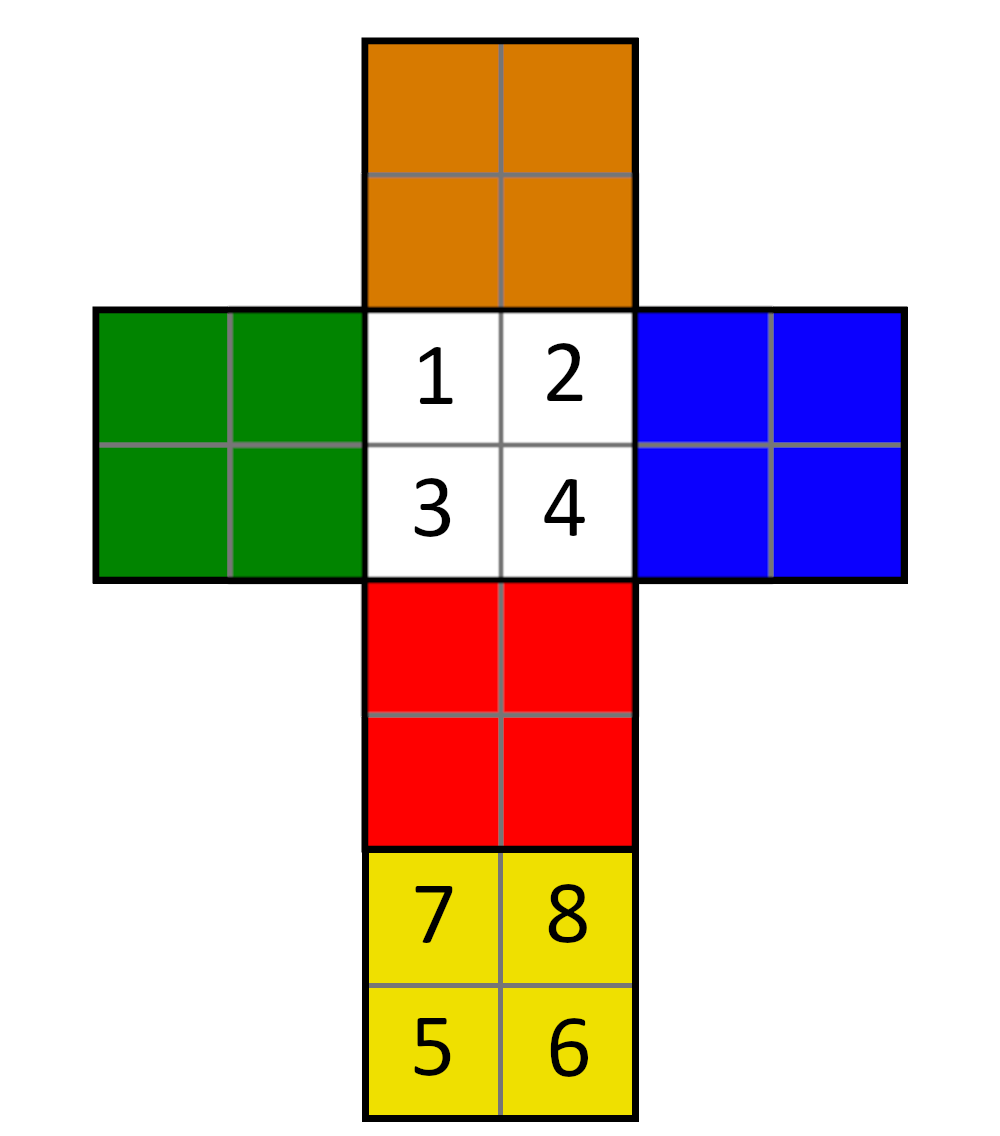
\includegraphics[scale=0.1]{foldedout_numbers.png}
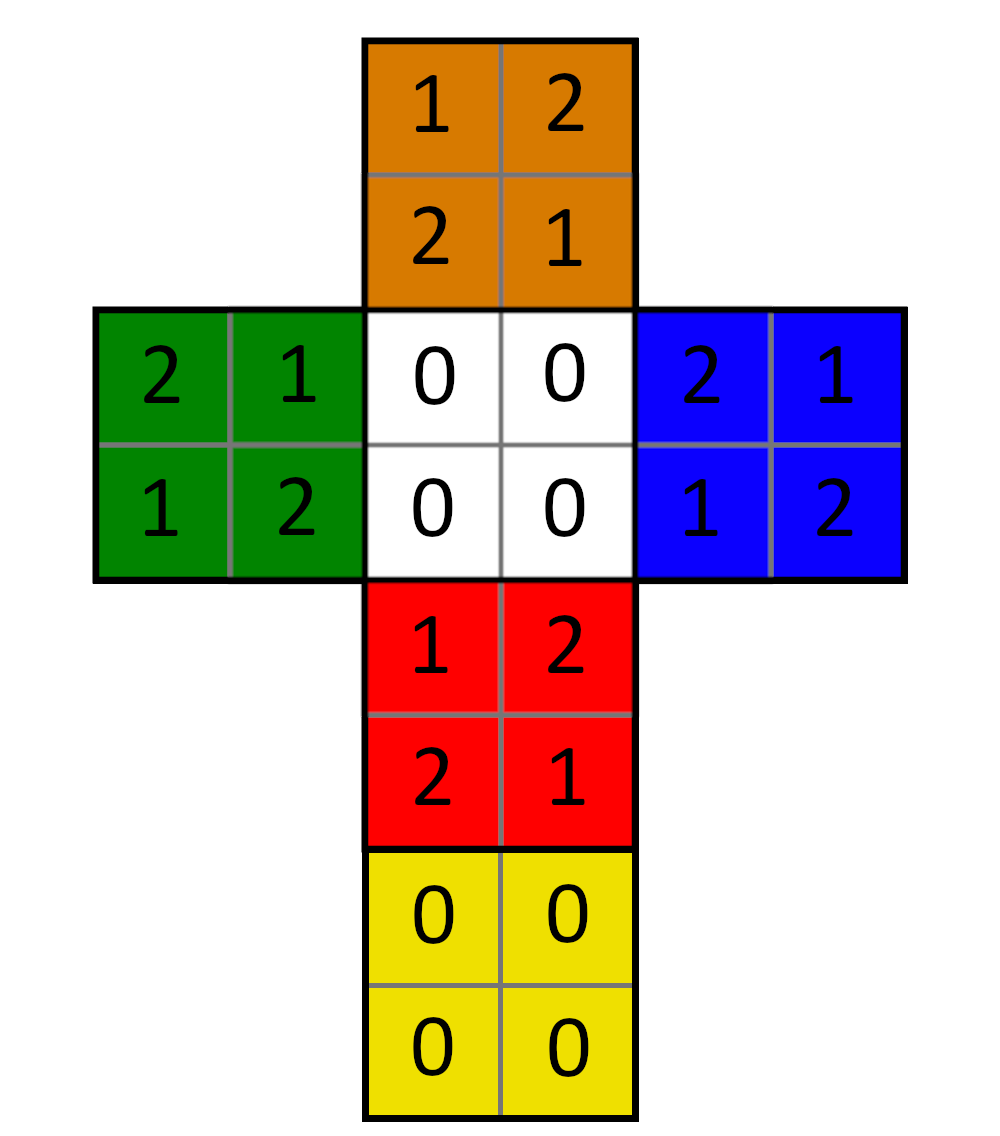
\includegraphics[scale=0.1]{foldedout_012.png}
\caption[Markierungen $x_i$ (links), Farbflächennummern (rechts)]{ausgeklappter Würfel mit Markierungen für $x_i$ (links) und Farbflächennummerierungen (rechts) }
\end{figure}
Außerdem bekommt jeder Stein an jeder Farbfläche eine Zahlenzuordnung. Da jeder Stein 3 Ausrichtungen haben kann, werden die Farbflächen mit 0, 1 und 2 nummeriert. Die Nummerierung beginnt mit der weißen bzw. gelben Fläche bei 0 und zählt dann im Uhrzeigersinn die Flächen. 
In der Startkonfiguration sind alle $x_i = 0$, der Vektor $x$ ist dann $(0, 0, 0, 0, 0, 0, 0, 0)$. Das wird kurz als $x=0$ geschrieben.

Nun wird der Zug $R$ als Beispiel ausgeführt (s. Abbildung \ref{Abbildung_XnachZugR}) und die Veränderung der Nummerierung der Farbflächen dargestellt. $R$ ist eine Rotation der rechten Ebene um 90$^\circ$ im Uhrzeigersinn. 
Die Kennzeichnungen $x_{1-8}$ bleiben an der gleichen Position, die Nummerierungen  der Farbflächen ändern sich mit Rotation der Ebene und ermöglichen so eine Zuordnung der Ausrichtung der Ecksteine. 
Die linke Seite der Würfels wird dabei nicht beeinflusst. Deshalb sind die Flächen an den Positionen $x_1, x_3, x_5, x_7$ alle 0. 
Die anderen Positionen haben nun aber andere Farbflächen: 
\begin{align*}
x_2 = 2 \ \ \ \ x_4 = 1 \ \ \ \ x_6 = 1 \ \ \ \ x_8 = 2  
\end{align*}
Daher gilt $x = (0, 2, 0, 1, 0, 1, 0, 2)$ nach dem Zug $R$. 
\begin{figure}[h]
\centering
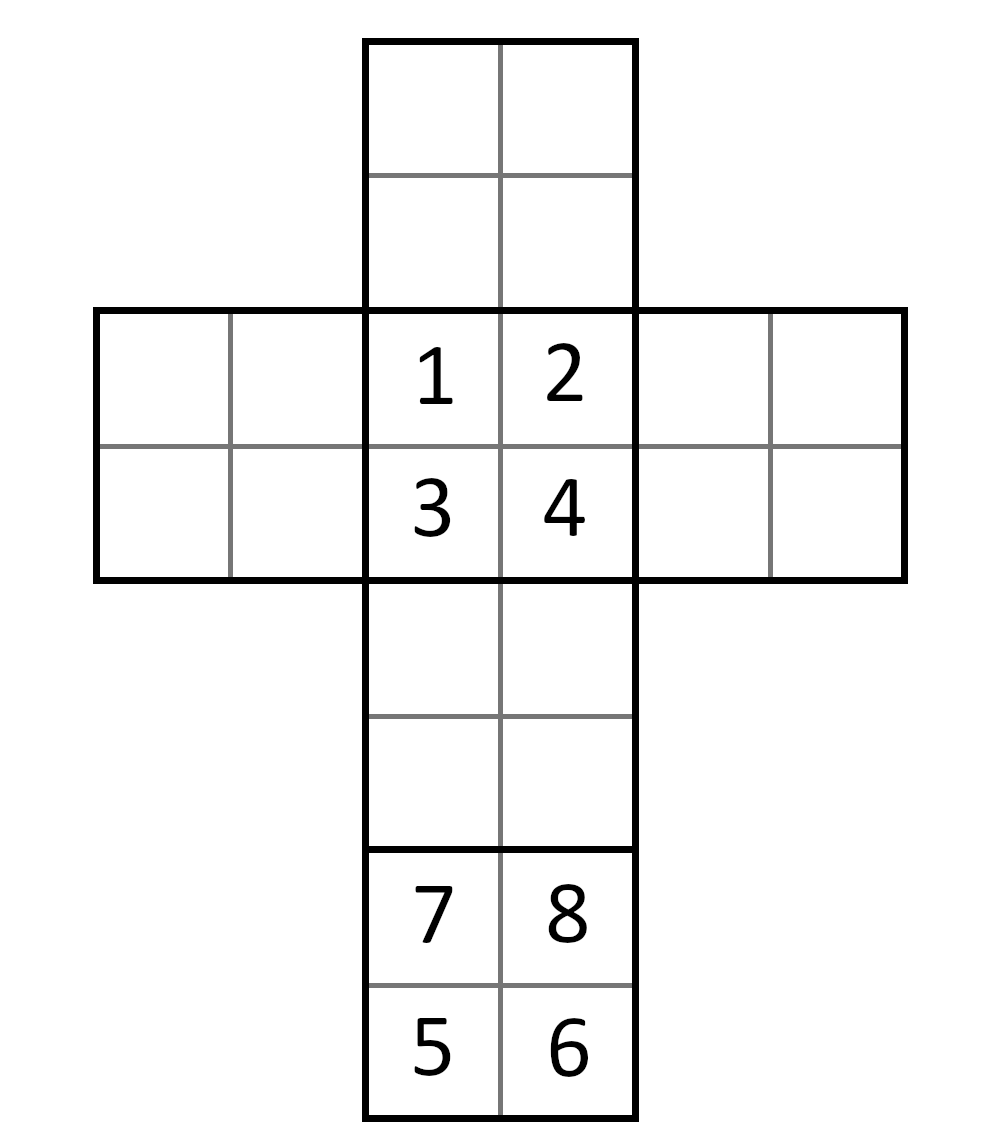
\includegraphics[scale=0.1]{foldedout_012_white.png}
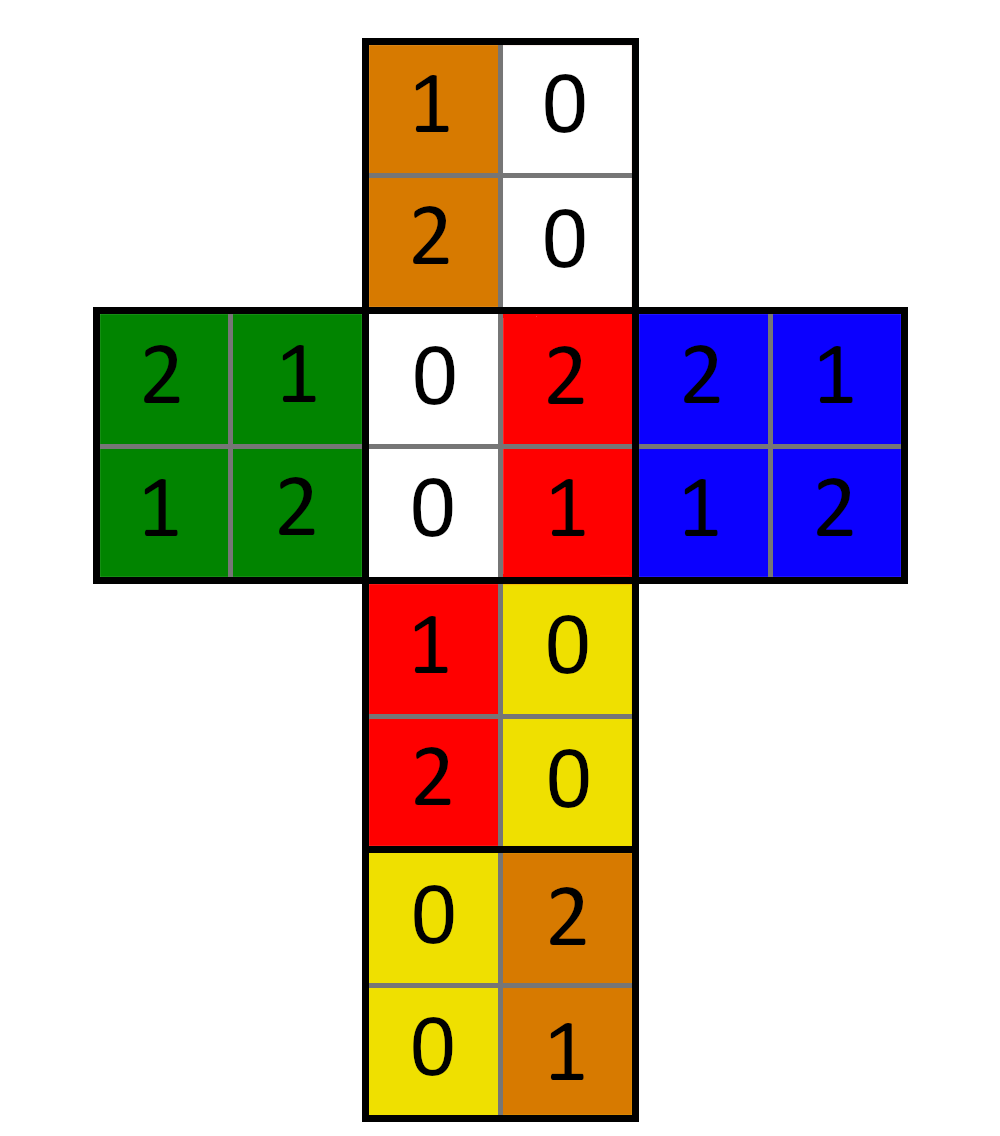
\includegraphics[scale=0.1]{foldedout_012_spin.png}
\caption[links: $x_1$ bis $x_8$, rechts: Veränderung nach dem Zug $R$]{links: Positionen $x_1$ bis $x_8$, rechts: Veränderung der nummerierten Ecksteine nach dem Zug $R$}
\label{Abbildung_XnachZugR}
\end{figure}

Anhand des Beispielzuges $R$ können Funktionen $f_R$ aufgestellt werden, die die Veränderung des Vektors $x$ nach Ausführen des Zuges $R$ bei jeder beliebigen Ausgangskonfiguration beschreiben. Da $x_1, x_3, x_5$ und $x_7$ nicht beeinfluss werden, bleiben diese unverändert.
\begin{align*}
f_{R_1}(x_1)=x_1 \ \ \ \ \ f_{R_3}(x_3)=x_3 \ \ \ \ \ f_{R_5}(x_5)=x_5 \ \ \ \ \ f_{R_6}(x_7)=x_7 
\end{align*}
Die Flächen an den Positionen $x_2, x_4, x_6$ und $x_8$ werden in Abhängigkeit der vorherigen Steinausrichtungen verändert. Es ergeben sich folgende Funktionen für die Positionen $x_2, x_4, x_6$ und $x_8$ nach dem Zug $R$: 


\begin{minipage}{0.5\textwidth}
\centering
$f_{R_2}(x_2)= \begin{cases}
2 & \ \text{falls } x_4 = 0 \\ 
0 & \ \text{falls } x_4 = 1 \\
1 & \ \text{falls } x_4 = 2 
\end{cases}$
\end{minipage}
\begin{minipage}{0.5\textwidth}
\centering
$f_{R_4}(x_4)= \begin{cases}
1 & \ \text{falls } x_8 = 0 \\ 
2 & \ \text{falls } x_8 = 1 \\
0 & \ \text{falls } x_8 = 2 
\end{cases}$
\end{minipage}

\begin{minipage}{0.5\textwidth}
\centering
$f_{R_8}(x_8)= \begin{cases}
2 & \ \text{falls } x_6 = 0 \\ 
0 & \ \text{falls } x_6 = 1 \\
1 & \ \text{falls } x_6 = 2 
\end{cases}$
\end{minipage}
\begin{minipage}{0.5\textwidth}
\centering
$f_{R_6}(x_6)= \begin{cases}
1 & \ \text{falls } x_2 = 0 \\ 
2 & \ \text{falls } x_2 = 1 \\
0 & \ \text{falls } x_2 = 2 
\end{cases}$
\end{minipage}


Es gibt für den Zug $R$ acht Funktionen $f_R$ -- eine für jeden Vektoreintrag. Die Funktionen $f_{R_2}$ und $f_{R_8}$ sind gleich, die Funktionen $f_{R_4}$ und $f_{R_6}$ ebenfalls. Auch die Funktionen $f_{R_1}, f_{R_3}, f_{R_5}$ und $f_{R_7}$ sind identisch. Da diese Funktionen gleich sind, reichen drei verschiedene Funktionen für die Veränderung von $x$ nach dem Zug $R$.


\begin{minipage}{0.4\textwidth}
\centering
$g(x)= \begin{cases}
2 & \ \text{falls } x = 0 \\ 
0 & \ \text{falls } x = 1 \\
1 & \ \text{falls } x = 2 
\end{cases}$
\end{minipage}
\begin{minipage}{0.4\textwidth}
\centering
$h(x)= \begin{cases}
1 & \ \text{falls } x = 0 \\ 
2 & \ \text{falls } x = 1 \\
0 & \ \text{falls } x = 2 
\end{cases}$
\end{minipage}
\begin{minipage}{0.2\textwidth}
\centering
$i(x) = x$
\end{minipage}

Da \textit{i} die Identitätsfunktion ist, kann diese weggelassen werden.
Mit den Funktionen \textit{g} und \textit{h} lassen sich die Ausrichtungen der Steine nach jedem Zug bestimmen. So wird der Vektor $x$ nach dem Zug $R$ durch die Funktion $\gamma_R$ verändert:
\begin{align*}
&& \gamma_R \left( (x_1, x_2, x_3, x_4, x_5, x_6, x_7, x_8  ) \right) \\ 
&& = \left( x_1, g(x_4), x_3, h(x_8), x_5, h(x_2), x_7, g(x_6) \right)
\end{align*}


%
%
%
%
%=======================================================================================================
%
%
%
%
%
%
\subsection*{Züge ausführen} \addcontentsline{toc}{subsection}{\protect\numberline{}Züge ausführen}

Eine Würfelkonfiguration $C=(\sigma, x)$ wird durch das Auführen eines Zuges verändert. Die Permutation $\sigma$ repräsentiert dann die neue Position der Steine im Würfel und $x$ die Ausrichtung der Steine. Ein Zug $Z$ kann dabei einer der Grundzüge ($U,D,R,L,F,B$) oder eine Aneinanderreihung von Grundzügen sein. Wird ein Zug $Z$ auf einer Würfelkonfiguration $C$ ausgeführt, wird das als $C \cdot Z$ geschrieben. Das Ergebnis von $C \cdot Z$ ist dann eine neue Folgekonfiguration $C$.

%
%
%
%
%
%
%=======================================================================================================
%
%
%
%
%
%
%
%

\newpage
\section{Würfel als Gruppe}

\label{Kapitel_WürfelAlsGruppe}

In diesem Kapitel wird die Gruppe des \Tthree \textit{Cubes} auf den \Ttwo \textit{Cube} übertragen. Die Gruppe des \Ttwo Würfels wird auf die vier Gruppenaxiome (Abgeschlossenheit, Assoziativität, Existenz eines neutralen Elements und Existenz eines inversen Elements) untersucht und auf Kommutativität untersucht.

Vorher wird die Rotation des Würfels und die Gleichheit zweier Züge durch Äquivalenz\-relationen und Äquivalenzklassen realisiert. Es werden auch die Ordnung und die Äquivalenz von Zügen berechnet.

%
%
%
%
%
%
%
%
%
%=======================================================================================================
%
%
%
%
%
%
%
%
%
%

\subsection*{Gleichheit von Zügen} \addcontentsline{toc}{subsection}{\protect\numberline{}Gleichheit von Zügen}

Zwei Züge $Z_1$ und $Z_2 \in A_Z$ gelten als gleich, wenn sie mit gleicher Ausgangskonfiguration des Würfels die gleiche Zielkonfiguration hervorrufen. $A_Z$ ist die Menge aller Züge.
Ein Zug besteht aus einem oder mehreren Grundzügen ($U, D, F, B, L, R$).
Das mehrfache Ausführen von Zügen kann mit der Exponentenschreibweise dargestellt werden. So wird beispielsweise $RR$ (zwei Drehungen der rechten Ebene im Uhrzeigersinn) auch als $R^2$ geschrieben.

Wenn eine Ebene vier mal hintereinander gedreht wird, ist der Würfel wieder in der vorherigen Position. Wenn der Würfel in einer Konfiguration $C = (\sigma, x)$ ist und ein Zug $Z \in \{ U^4, D^4, R^4, L^4, F^4, B^4\} $ ausgeführt wird, ist die Folgekonfiguration wieder $C$.
\begin{align*}
C \cdot Z = C  \text{ mit } Z \in \{ U^4, D^4, R^4, L^4, F^4, B^4\} \text{ und } C \text{ als Würfelkonfiguration}
\end{align*}
Das bedeutet, dass jeder Zug $Z = Z_1Z_2Z_3$ mit $Z_2 \in \{ U^4, D^4, R^4, L^4, F^4, B^4\}$ die gleiche Konfiguration wie der Zug $Z_1Z_3$ hervorruft.
Der Exponent kann in diesem Fall $modulo \ 4$ gerechnet, da vier Drehungen einer Ebene nacheinander wieder zum Startzustand führen. 
Es gilt folglich:
\begin{align*}
\forall \  Z \in \{U, D, F, B, L, R\}, n \in \mathbb{N} \ . \ Z^n=Z^{n \mod 4}
\end{align*}
Dabei gilt für $n \mod 4 = 0$ dann $Z^n = Z^{n \mod 4} = Z^0$. $Z^0$ repräsentiert dabei einen leeren Zug. Das entspricht keiner Veränderung der Folgekonfiguration des Würfels.

Da die Anzahl der möglichen Züge im Gegensatz zur Anzahl der validen Würfelkonfigurationen (s. Kapitel \ref{Kapitel_ValideKonfigurationen}) unendlich ist, gibt es viele Fälle, in denen zwei Züge die gleiche Folgekonfiguration hervorrufen und somit als gleich gelten. Dies wird im weiteren Verlauf dieser Arbeit durch Äquivalenzklassen realisiert.


%
%
%
%
%=======================================================================================================
%
%
%
%
%
%

\subsection*{Rotation des Würfels}\addcontentsline{toc}{subsection}{\protect\numberline{}Rotation des Würfels}

Der \Ttwo Würfel hat im Gegensatz zum \Tthree Würfel keine Mittelsteine, die fest darüber entscheiden, welche Seite die obere Seite ist. 
Der \Ttwo Würfel kann daher im gelösten Zustand sein, ohne dass die obere Seite weiß ist. Deshalb muss es möglich sein, den Würfel ganz zu rotieren, ohne einen Zug auszuführen.
Das soll im nächsten Abschnitt als Äquivalenrelationen umgesetzt werden. Dafür werden die Rotationsmöglichkeiten des Würfels in diesem Abschnitt definiert.
Um die Drehungen zu benennen, werden die Achsen des Würfels als $x, y$ und $z$ definiert. Das ist in Abbildung \ref{Abbildung_Rotationsachsen} zu sehen.
\begin{figure}[h]
\centering
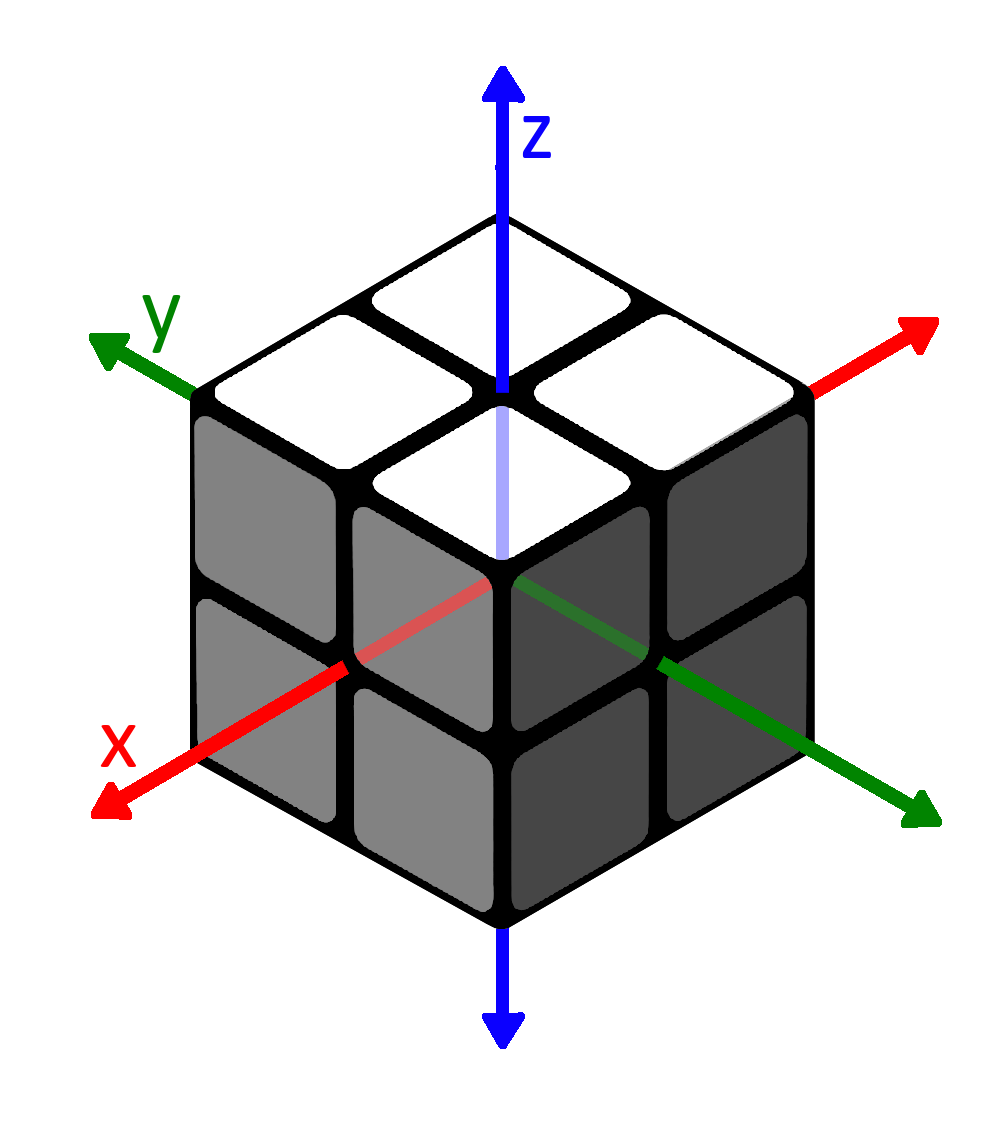
\includegraphics[scale=0.13]{Pfeile.png}
\caption[Würfel mit $x, y$ und $z$-Achsen]{Würfel mit $x, y$ und $z$-Achsen}
\label{Abbildung_Rotationsachsen}
\end{figure} 

Nun können für die möglichen Rotationen des Würfels Nachfolgekonfigurationen festgelegt werden. 
Dazu werden zuerst die einzelnen Rotationen des Würfels benannt. 

\begin{tabular}{cl}
\toprule
\textbf{Abkürzung} & \textbf{Beschreibung der Rotation} \\
\midrule
$Z_l$ & Rotation des Würfels um die $z$-Achse nach links (gegen den Uhrzeigersinn)\\

$Z_r$ & Rotation des Würfels um die $z$-Achse nach rechts (im Uhrzeigersinn)  \\

$Y_l$ & Rotation des Würfels um die $y$-Achse nach links (gegen den Uhrzeigersinn)\\

$Y_r$ & Rotation des Würfels um die $y$-Achse nach rechts (im Uhrzeigersinn)  \\

$X_l$ & Rotation des Würfels um die $x$-Achse nach links (gegen den Uhrzeigersinn)\\

$X_r$ & Rotation des Würfels um die $x$-Achse nach rechts (im Uhrzeigersinn) \\

$N_R$ & keine Rotation des Würfels \\
\bottomrule
\end{tabular} 


Die Rotationen sind nicht minimal definiert, da beispielsweise $Z_l$ das gleiche wie ${Z_r}^3$ ist. Dies dient der Anschaulichkeit. 

Die Steine werden durch eine Rotation alle an einen neuen Platz gebracht. Anders als bei der Drehung der Ebenen, wo nur einige Steine die Position ändern, ändern hier alle Steine die Position, ohne dass der Würfel verändert wird, da er komplett gedreht wird. 

Anhand der Rotation $Z_r$, also einer Rotation des kompletten Würfels um die $z$-Achse um $90^\circ$ im Uhrzeigersinn, wird nun die Veränderung der Würfelpositionen gezeigt. Die Rotation $Z_r$ ist in Abbildung \ref{Abbildung_WürfelNachRotationUmZAchse} zu sehen.
\begin{figure}[H]
\centering
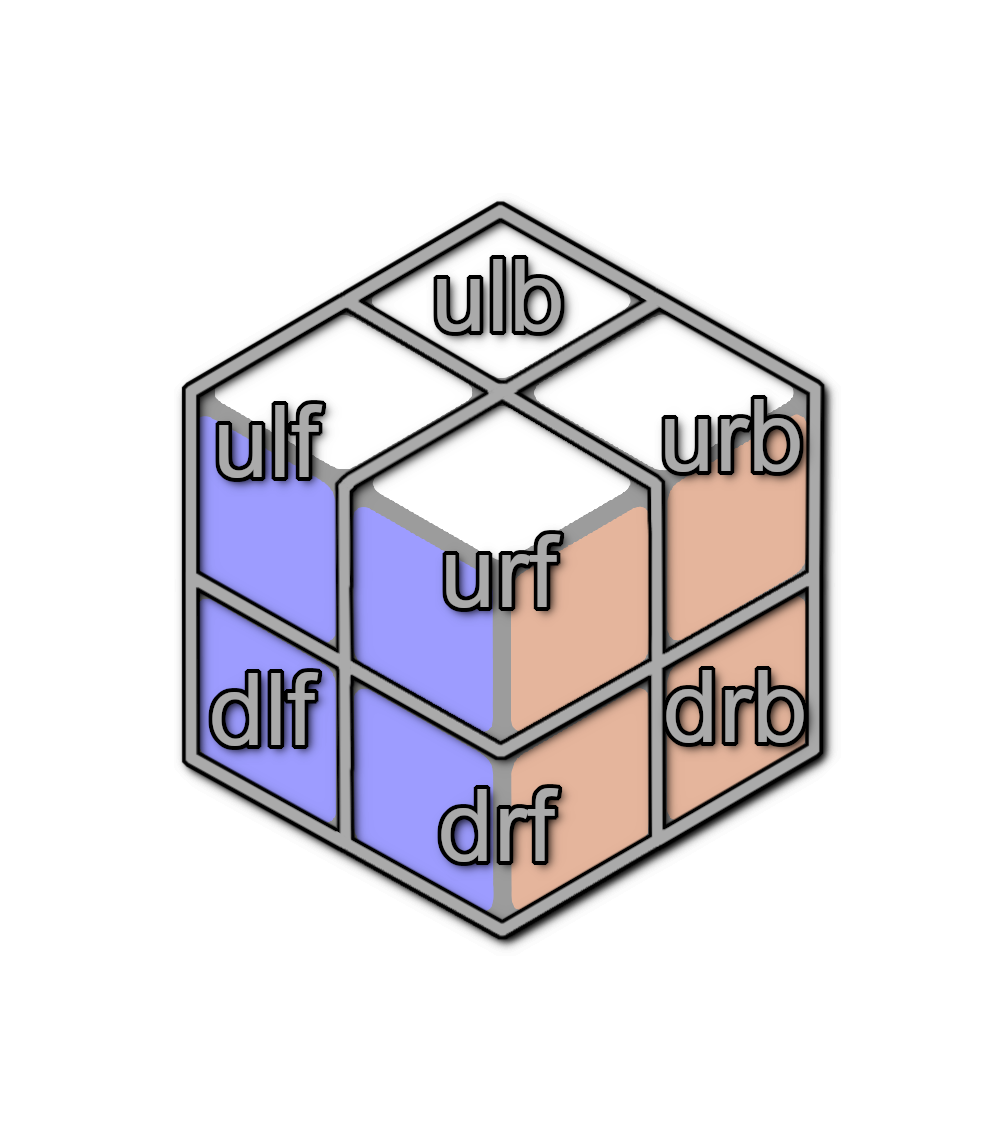
\includegraphics[scale=0.13]{auf_ulf.png}
\caption{Würfel nach Rotation um $z$-Achse}
\label{Abbildung_WürfelNachRotationUmZAchse}
\end{figure}
Da bei den Rotationen alle Steine die Position wechseln, muss es demnach 8 Funktionen $\delta$ geben, also für jeden Eckstein eine Funktion $\delta$:
\begin{alignat*}{4}
& \delta_{Z_r}(\textit{urf}) = \textit{ulf} \ \ \ \ \ \ & \delta_{Z_r}(\textit{ulf}) = \textit{ulb} \ \ \ \ \ \ & \delta_{Z_r}(\textit{ulb}) = \textit{urb} \ \ \ \ \ \ & \delta_{Z_r}(\textit{urb}) = \textit{urf} \\
& \delta_{Z_r}(\textit{drf}) = \textit{dlf} \ \ \ \ \ \ & \delta_{Z_r}(\textit{dlf}) = \textit{dlb} \ \ \ \ \ \ \ & \delta_{Z_r}(\textit{dlb}) = \textit{drb} \ \ \ \ \ \ & \delta_{Z_r}(\textit{drb}) = \textit{drf}
\end{alignat*}

Das kann nun in der Form $i \mapsto j$ geschrieben werden: 
\begin{alignat*}{4}
& \textit{urf} \mapsto \textit{ulf} \ \ \ \ \ \ \ \ & \textit{ulf} \mapsto \textit{ulb} \ \ \ \ \ \ \ \ & \textit{ulb} \mapsto \textit{urb} \ \ \ \ \ \ \ \ & \textit{urb} \mapsto \textit{urf} \\
& \textit{drf} \mapsto \textit{dlf} \ \ \ \ \ \ \ \ & \textit{dlf} \mapsto \textit{dlb} \ \ \ \ \ \ \ \ \ & \textit{dlb} \mapsto \textit{drb} \ \ \ \ \ \ \ \ & \textit{drb} \mapsto \textit{drf}
\end{alignat*}

In der Zykel-Schreibweise sieht die Veränderung der Steinnamen dann so aus: \\
$\delta_{Z_r}=( \ \textit{urf} \ \textit{ulf} \ \textit{ulb} \ \textit{urb} \ )( \ \textit{drf} \ \textit{dlf} \ \textit{dlb} \ \textit{drb} \  )$ 

Alle Rotationen sehen in Zykel-Schreibweise folgendermaßen aus:
\begin{align*}
\delta_{Z_r} & = ( \ \textit{ulf} \ \textit{ulb} \ \textit{urb} \ \textit{urb}) \ (\textit{dlf} \ \textit{dlb} \ \textit{drb} \ \textit{drf} \ )\\
\delta_{Z_l} & = ( \ \textit{ulf} \ \textit{urf} \ \textit{urb} \ \textit{ulb}) \ (\textit{dlf} \ \textit{drf} \ \textit{drb} \ \textit{dlb} \ )\\
\delta_{Y_r} & = ( \ \textit{ulf} \ \textit{ulb} \ \textit{dlb} \ \textit{dlf}) \ (\textit{urf} \ \textit{urb} \ \textit{drb} \ \textit{drf} \ )\\
\delta_{Y_l} & = ( \ \textit{ulf} \ \textit{dlf} \ \textit{dlb} \ \textit{ulb}) \ (\textit{urf} \ \textit{drf} \ \textit{drb} \ \textit{urb} \ )\\
\delta_{X_r} & = ( \ \textit{ulf} \ \textit{urf} \ \textit{drf} \ \textit{dlf}) \ (\textit{urb} \ \textit{ulb} \ \textit{dlb} \ \textit{drb} \ )\\
\delta_{X_l} & = ( \ \textit{ulf} \ \textit{dlf} \ \textit{drf} \ \textit{urf}) \ (\textit{urb} \ \textit{ulb} \ \textit{dlb} \ \textit{drb} \ )
\end{align*}
Bei den Rotationen wird (analog zu den Zügen) die mehrfache Ausführung einer Roatation mit der Exponentenschreibweise geschrieben. 
Somit gilt dann auch hier $TTTT=T^4=N_R$ (für $R \in \{{Z_r}, {Z_l}, {Y_r}, {Y_l}, {X_r}, {X_l} , H_R \}$) und $T^0=N_R$ (für alle Rotationen). ($N_R$ ist die leere Rotation und $T$ ist eine beliebige Rotation des Würfels.) 
Analog zu den Zügen gilt bei den Rotationen dementsprechend für jede Rotation: 
\begin{align*}
\forall T \in \{{Z_r}, {Z_l}, {Y_r}, {Y_l}, {X_r}, {X_l}, N_R \}, n \in \mathbb{N} \ . \ T^n=T^{n \mod 4}
\end{align*}


%
%
%
%
%
%
%
%
%
%
%=======================================================================================================
%
%
%
%
%
%
%
%
%
%
\color{black}

\subsection*{Äquivalenzrelation der Züge}\addcontentsline{toc}{subsection}{\protect\numberline{}Äquivalenzrelationen der Rotationen}

Da der \Ttwo Würfel im Gegensatz zum \Tthree Würfel keine feste Ausrichtung hat, werden in diesem Abschnitt Äquivalenzrelationen eingeführt, um die Rotationen des Würfels umzusetzen.
Für Äquivalenzrotaionen müssen die drei folgenden Eigenschaften gelten: Reflexivität, Symmetrie, Transitivität. In Kapitel \ref{Abschnitt_Äquivalenrelationen} findet sich die Definition und Erklärung.

In dem Fall des \Ttwo Würfels handelt es sich um eine Relation von zwei Zügen $Z_1, Z_2$ aus der Menge aller Züge $A_Z$. 

Die Äquivalenzrelation der Rotation wird hier so definiert: 


\begin{tabular}{l l}
$Z_1 \sim Z_2 := \ $  & $Z_1$ \textit{und} $Z_2$ \textit{ergeben (mit optionaler Rotation) die gleiche }\\
\  & \textit{Würfelkonfiguration} \\
\end{tabular} 
\\

Die Relation $\sim$ prüft zwei Züge $Z_1$ und $Z_2$ auf Gleichheit und berücksichtigt dabei gleichzeitig die Rotation des Würfels.

Daraus ergibt sich $Z_1 \sim Z_2 :\Leftrightarrow \ C \cdot Z_1 = C \cdot WZ_2$ mit $C$ als Würfelkonfiguration und $W$ als Element (oder Kombination von Elementen) aus $\{{Z_r}, {Z_l}, {Y_r}, {Y_l}, {X_r}, {X_l}, N_R\}$ -- wobei $N_R$ die \textit{leere} Rotation darstellt, das entspricht keiner Rotation des Würfels. 
Somit ergibt sich beispielsweise $F \sim L \Leftrightarrow C \cdot F = C \cdot Z_rL$, da eine Drehung der vorderen Ebene und eine Drehung des Würfels nach links mit einer Drehung der linken Ebene die gleiche Würfelkonfiguration ergeben. Der Würfel ist dann nur verschieden ausgerichtet. 
In Abbildung \ref{Abbildung_GelöstnachFnachZL} ist dieses Beispiel nochmal grafisch dargestellt: Links befindet sich der gelöste Würfel, in der Mitte der gelöste Würfel nach dem Zug $F$ und rechts der gelöste Würfel nach dem Zug $Z_rL$. Die beiden rechten Würfel sind in der gleichen Konfigurationen, aber anders gedreht.
\begin{figure}[h]
\centering
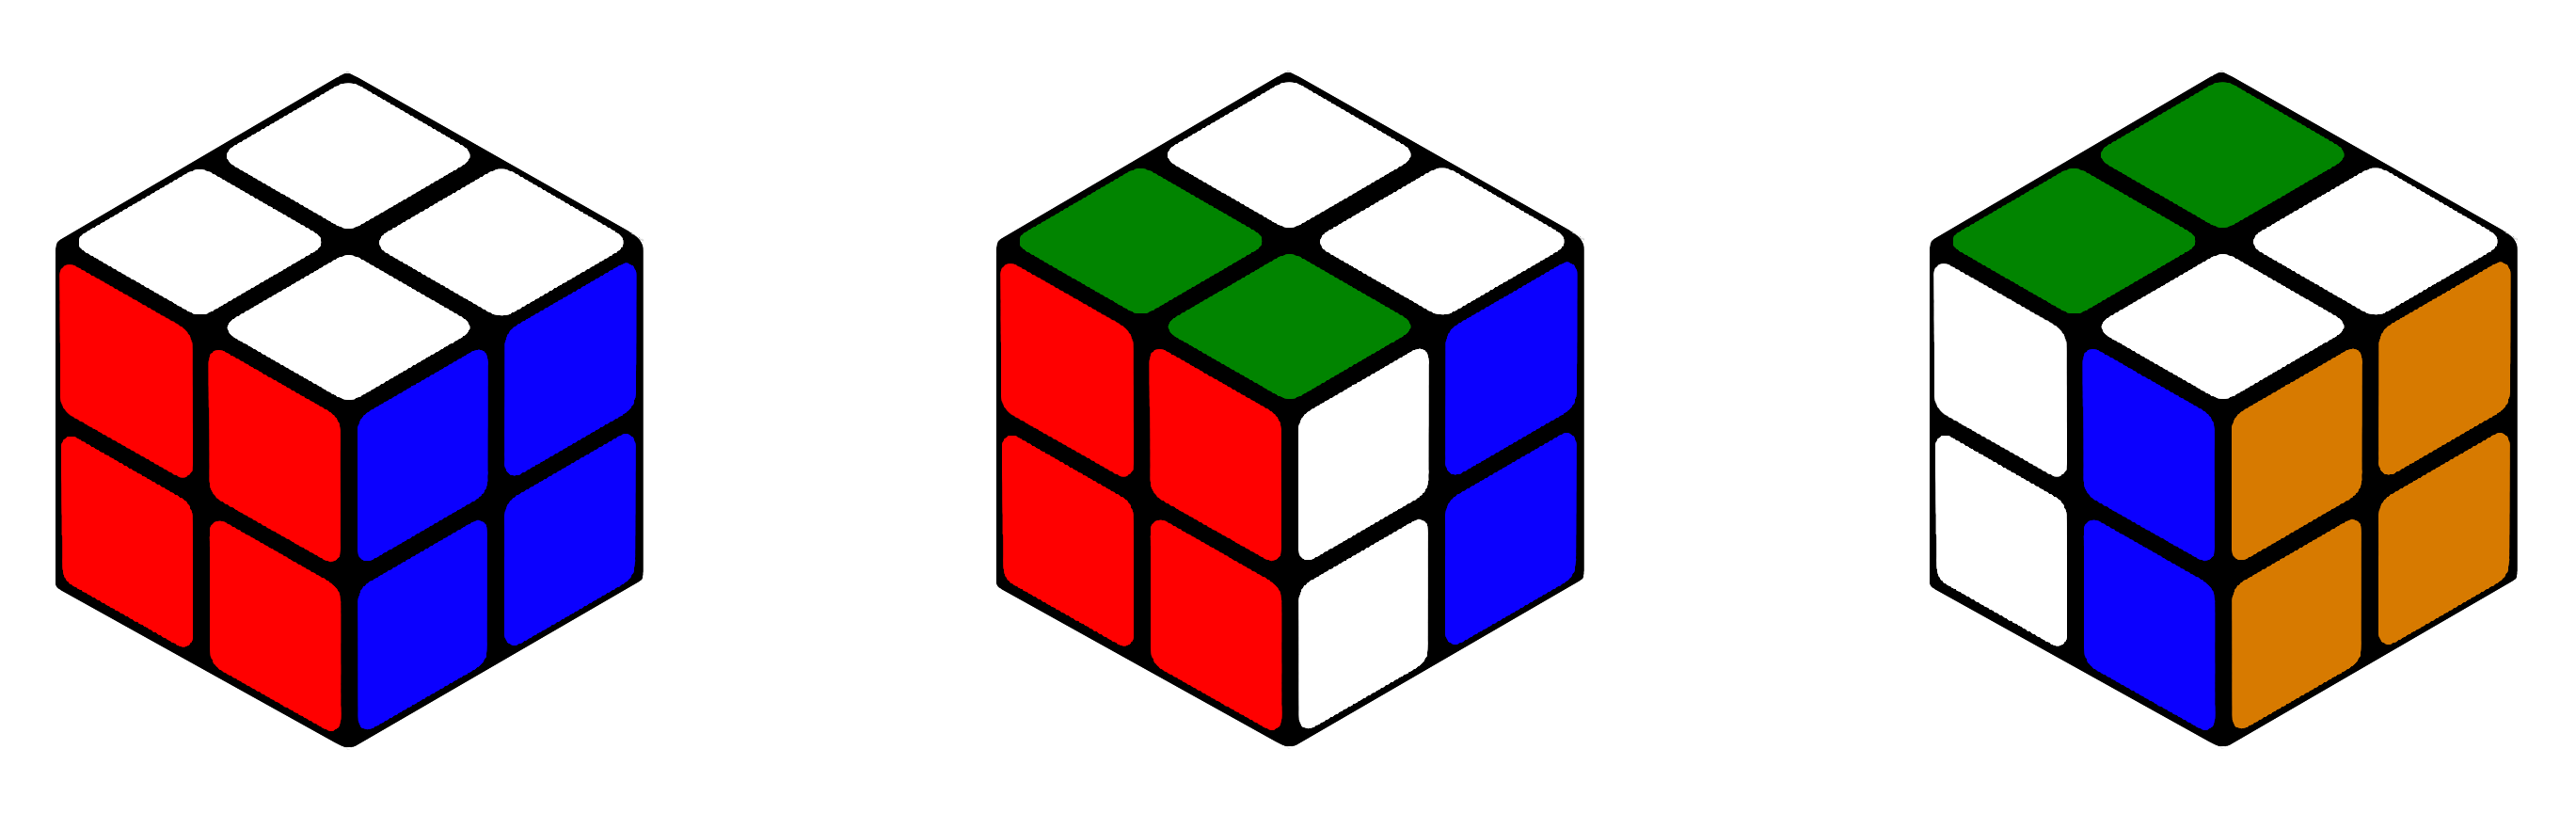
\includegraphics[scale=0.15]{3_wuerfel.png}
\caption[Würfel gelöst, nach Zug $F$ und nach $Z_rL$]{Würfel gelöst (links), nach Zug $F$ (mitte) und nach $Z_rL$(rechts)}
\label{Abbildung_GelöstnachFnachZL}
\end{figure}

Damit $\sim$ eine Äquivalenzrelation ist, müssen Reflexivität, Symmetrie und Transitivität gelten, was im folgenden Abschnitt bewiesen wird.

\begin{description}


\item [Reflexivität] \ \\
Für die Reflexivität muss $Z \sim Z$ für alle Züge gelten. 
\begin{align*}
Z_1 \sim_R Z_2 : & \Leftrightarrow C \cdot Z_1 = C \cdot WZ_2
\end{align*}
Es wird $W$ als $N_R$ gewählt, so dass keine Rotation ausgeführt wird.
\begin{align*}
Z_1 \sim Z_2 : & \Leftrightarrow  C \cdot Z_1 = C \cdot WZ_2 \\
\ & \Leftrightarrow C \cdot Z_1=C \cdot N_R Z_2 \\
\ & \Leftrightarrow C \cdot Z_1 = C \cdot Z_2
\end{align*}
Es gilt somit die Reflexivität für $\sim$, da für $Z_1 \sim Z_2$ mit $W=N_R$ $Z_1$ und $Z_2$ immer äquivalent sind, da sie die gleiche Folgekonfiguration des Würfels erreichen.

\item [Symmetrie] \ \\
Für die Symmetrie muss gelten: Aus $Z_1 \sim Z_2$ folgt $Z_2 \sim Z_1$.
\begin{align*}
Z_1 \sim Z_2 & \Rightarrow Z_2 \sim Z_1 \\
mit \ Z_1 \sim Z_2 : & \Leftrightarrow  C \cdot  Z_1 = C \cdot  WZ_2 \\
\Leftrightarrow C \cdot  Z_1 = C \cdot  W_1 Z_2 & \Rightarrow C \cdot  Z_2 = C \cdot  W_2 Z_1
\end{align*}
Das gilt, wenn $W_2$ das Inverse von $W_1$ ist. Das Inverse ist die Rotation um die gleiche Achse, aber in die andere Richtung. 
Das Inverse von $W$ wird als $W^{-1}$ geschrieben.
Das sind die Rotationen mit den dazugehörigen Inversen:

\begin{center}
\begin{tabular}{lccccccc}
Rotation $W$ & ${Z_r}$ & ${Z_l}$ &  ${Y_r}$ & ${Y_l}$ & ${X_r}$ & ${X_l}$ & $N_R$ \\
\hline
Inverses \hspace*{0.1em} $W^{-1}$ & ${Z_l}$ & ${Z_r}$ &  ${Y_l}$ & ${Y_r}$ & ${X_l}$ & ${X_r}$ & $N_R$ \\
\end{tabular} 
\end{center}
Dann gilt: 
\begin{align*}
C \cdot  Z_1 = C \cdot  W Z_2 & \Rightarrow C \cdot  Z_2 = C \cdot  W^{-1} Z_1
\end{align*}
Das gilt, da durch $W^{-1}$ der Würfel in die entgegengesetzte Richtung rotiert wird und die Züge somit wieder die gleiche Würfelkonfiguration ergeben.
Folglich gilt die Symmetrie für $\sim$.


\item [Transitivität] \ \\
Es muss gelten: Aus $Z_1 \sim Z_2$ und $Z_2 \sim Z_3$ folgt $Z_1 \sim Z_3$.
\begin{alignat*}{3}
& Z_1 \sim Z_2 && \wedge Z_2 \sim Z_3 && \Rightarrow Z_1 \sim Z_3 \\
\Leftrightarrow \ & C \cdot  Z_1 = C \cdot  W_1Z_2 \ && \wedge C \cdot  Z_2 = C \cdot  W_2Z_3 \ && \Rightarrow C \cdot  Z_1 = C \cdot  W_3Z_3
\end{alignat*}
Das gilt für $W_3=W_1W2$.
\begin{alignat*}{3}
\Leftrightarrow \ & C \cdot  Z_1 = C \cdot  W_1Z_2 \ && \wedge C \cdot  Z_2 = C \cdot W_2Z_3 \ && \Rightarrow C \cdot  Z_1 = C \cdot W_1W_2Z_3 
\end{alignat*}
Da die Züge $Z_1$ und $Z_2$ mit der Rotation $W_1$ die gleiche Würfelkonfiguration ergeben, und die Züge $Z_2$ und $Z_3$ nach der Rotation $W_2$ auch die gleiche Würfelkonfiguration ergeben, gilt das auch für die beiden Züge $Z_1$ und $Z_3$ nach der Rotation $W_3=W_1W_2$, da dann alle nötigen Rotationen durchgeführt wurden.

\end{description}




%
%
%
%
%
%
%
%
%
%
%=======================================================================================================
%
%
%
%
%
%
%
%
%
%


\subsection*{Äquivalenzklassen} \addcontentsline{toc}{subsection}{\protect\numberline{}Äquivalenzklassen}

Äquivalenzklassen und Faktormengen wurden in Kapitel \ref{Abschnitt_FaktormengenUndÄquivalenzklasse} eingeführt. In diesem Abschnitt werden die Äquivalenzklassen der Relation $\sim$ auf der Menge aller Züge $A_Z$ definiert. Die Menge der Äquivalenzklassen, die durch $A_Z / \sim$ entstehen wird $\Gtwo$ genannt. Sie enthält alle die Äquivalenklassen aller validen Würfelzüge, ohne dabei gleiche Züge oder Würfelrotationen doppelt zu enthalten. Die Elemente von $\Gtwo$ sind definiert als $\{[Z] \mid Z \in A_Z \}$. Im weiteren Verlauf dieser Arbeit werden die eckigen Klammern der Äquivalenzklassen in $\Gtwo$ aber weggelassen, um die Notation zu verreinfachen. $\Gtwo$ enthält alle möglichen Züge des Würfels ohne dabei doppelte Züge zu enthalten.

%
%
%
%
%
%
%
%
%
%=======================================================================================================
%
%
%
%
%
%
%
%
%
%

\subsection*{\Ttwo Zauberwüfel als Gruppe} \addcontentsline{toc}{subsection}{\protect\numberline{}\Ttwo Zauberwüfel als Gruppe} \label{Abschnitt_WürfelAlsGruppe}

Im Folgenden wird die Definition der Gruppe des \Tthree Würfels aus \textit{Group Theory and the Rubik's Cube}  von Janet Chen \cite{JC} als Gruppe des \Ttwo Würfels umgesetzt. Die Gruppe von Janet Chen wird hier als $(\Gthree, *)$ bezeichnet, auch wenn er sie als $(G, *)$ bezeichnet hat. Der Namen der Gruppe wird geändert, um klar zwischen dem \Ttwo  und dem \Tthree Würfel zu differenzieren. Die Gruppe des \Ttwo Würfels heißt $(\Gtwo, \circ)$. 
Die Grundlagen und Definition der Gruppe wurden in Kapitel \ref{Abschnitt_Gruppe} erklärt.


Die Menge $\Gtwo$ besteht aus allen möglichen Zügen des Würfels, ohne doppelte Züge zu enthalten. Das wurde bereits durch Äquivalenzklassen realisiert. Beispielsweise die Drehung der oberen Ebene ist ein Zug. Ein Zug kann aber auch aus mehreren Drehungen bestehen, z.B. das Drehen der oberen Ebene, gefolgt von dem Drehen der rechten Ebene stellt ebenfalls einen Zug dar. 


Der Operator $\circ$ ist als Konkatenation zweier Züge definiert. Wenn $Z_1 \in \Gtwo$ und $Z_2 \in \Gtwo$ zwei Züge sind, dann bedeutet $Z_1 \circ Z_2$, dass zuerst $Z_1$ und dann $Z_2$ ausgeführt wird. (Außerdem gilt dann auch $Z_1 \circ Z_2 \in \Gtwo$.) $Z_1 \circ Z_2$ kann auch als $Z_1Z_2$ geschrieben werden.

Im Folgenden wird gezeigt, dass $(\Gtwo, \circ)$ eine Gruppe ist, indem $(\Gtwo, \circ)$ bezüglich der Gruppenkriterien untersucht wird:
\begin{description}
\item [Abgeschlossenheit] \ \\
$\forall Z_1,Z_2 \in \Gtwo .  (Z_1 \circ Z_2) \in \Gtwo $ 


Die Gruppe $\Gtwo$ ist abgeschlossen unter dem Operator $\circ$. Wenn $Z_1 $ und $Z_2$ Züge sind und somit Elemente von $\Gtwo$, dann ist auch $Z_1 \circ Z_2$ ein Element der Gruppe, da alle Züge in $\Gtwo$ enthalten sind. In $\Gtwo$ findet sich zu jeder validen Würfelkonfiguration ein Zug, um diese zu erreichen und jede Verknüpfung von zwei validen Zügen führt zu einer validen Würfelkonfiguration. Daher gilt die Abgeschlossenheit bei der Gruppe $(\Gtwo, \circ)$.



\item [Assoziativität] \ \\
$\forall Z_1,Z_2,Z_3 \in \Gtwo.(Z_1 \circ Z_2) \circ Z_3 = Z_1 \circ (Z_2 \circ Z_3)$ 


Um die Assoziativität zu zeigen, wird eine Schreibweise für das Ausführen der Züge eingeführt. Ein beliebiger, fester Stein im Würfel wird $s$ genannt. Beim Ausführen eines Zuges $Z$ wird nun $Z(s)$ geschrieben, um die neue Position des Steines zu erhalten. Die Positionen sind (wie oben beschrieben) 3-Buchstaben-Kürzel, bestehend aus $u, d, l, r, t, b$. 

Bei der Betrachtung von $Z_1 \circ Z_2 $, wird zuerst $Z_1$ und dann $Z_2$ ausgeführt. $Z_1(s)$ bewegt den Stein s zu der Position $Z_1(s)$. Der Zug $Z_2$ bewegt den Stein dann zu der Position $Z_2(Z_1(s))$. Folglich gilt $Z_1 \circ Z_2 = Z_2(Z_1(s))$. 


Nun muss noch $(Z_1 \circ Z_2) \circ Z_3 = Z_1 \circ (Z_2 \circ Z_3)$ gezeigt werden. Dafür wird gezeigt, dass sich $(Z_1 \circ Z_2) \circ Z_3$ und $Z_1 \circ (Z_2 \circ Z_3)$ beide zu $Z_3(Z_2(Z_1(s))$ umformen lassen: 
\begin{align*}
& (Z_1 \circ Z_2) \circ Z_3  \\
\Leftrightarrow (&(Z_1 \circ Z_2) \circ Z_3)(s) \\
= & Z_3(Z_1 \circ Z_2)(s)) \\
= & Z_3(Z_2(Z_1(s)))  
\end{align*}
\begin{align*}
&Z_1 \circ (Z_2 \circ Z_3) \\
\Leftrightarrow (&Z_1 \circ (Z_2 \circ Z_3))(s) \\
= (&Z_2 \circ Z_3)(Z_1(s)) \\
= \ \ & Z_3(Z_2(Z_1(s)))  
\end{align*}
Somit ist $(\Gtwo, \circ)$ assoziativ.

\item [Existenz eines neutralen Elements $N$] \ \\
$\forall Z_1 \in \Gtwo, \exists N \in \Gtwo.N \circ Z_1 = Z_1 \circ N = Z_1$ 


Das neutrale Element $N$ muss aus der Menge $\Gtwo$ der Züge sein und es muss gelten: $N \circ Z_1 = Z_1 \circ N = Z_1$. Somit ist das neutrale Element der Gruppe $(\Gtwo, \circ)$ der \textit{leere} Zug. Es werden dabei keine der Ebenen des Würfels gedreht. Wenn ein Zug $Z$ ausführt wird und dann der Zug $N$, bedeutet das \textit{erst $Z$ ausführen und dann nichts}, was das gleiche ist wie \textit{$Z$ auszuführen}.


Wenn eine Ebene beispielsweise vier mal gedreht wird, ist der Würfel wieder in der vorherigen Position. Somit gilt beispielsweise $RRRR=R^4=N$, wobei $N$ für das neutrale Element (bzw. den leeren Zug) steht. Das gilt für alle Züge des Würfels:

\begin{align*}
RRRR & =R^4 =N \\
LLLL & =L^4 =N \\
UUUU & =U^4 =N \\
DDDD & =D^4 =N \\
FFFF & =F^4 =N \\
BBBB & =B^4 =N \\
\end{align*}
Diese sind dann alle Repräsentanten für den leeren Zug $N$ enthalten.
Somit gilt dann auch $Z^0=N$, mit $Z$ als beliebigen Zug und $N$ als neutrales Element. 

Das neutrale Element $N$ von $(\Gtwo, \circ)$ ist also der leere Zug bzw. jeder Repräsentant der Äquivalenzklasse des leeren Zuges.


\item [Existenz eines inversen Elements $Z^{-1}$] \ \\
$\forall \  Z \in \Gtwo,\ \exists \  Z^{-1} \in \Gtwo.  \ \ Z \circ Z^{-1} = Z^{-1} \circ Z = N$  


Da jeder Zug $Z$ als Permutation definiert ist, kann diese invertiert werden. Wenn man eine Permutation invertieren will, kehrt man die Reihenfolge der Elemente der Zykel um. Heraus kommt bei einer Verknüpfung dieser beiden Permutationen das die Identitätspermutation bzw. das neutrale Element.
Somit gilt dann $Z \circ Z^{-1} = Z^{-1} \circ Z = N$.
\end{description}
Somit ist $(\Gtwo, \circ)$ eine Gruppe. 


$(\Gtwo, \circ)$ ist keine kommutative Gruppe, da beispielsweise eine Rotation der rechten Ebene im Uhrzeigersinn ($R$) und eine Rotation der vorderen Ebene im Uhrzeigersinn ($F$) in umgekehrter Reihenfolge ein anderes Ergebnis haben. Das ist in Abbildung \ref{Abbildung_WürfelNachFRundRF} grafisch dargestellt oder kann einfach händisch an einem Würfel ausprobiert werden.
\begin{figure}[h]
\centering
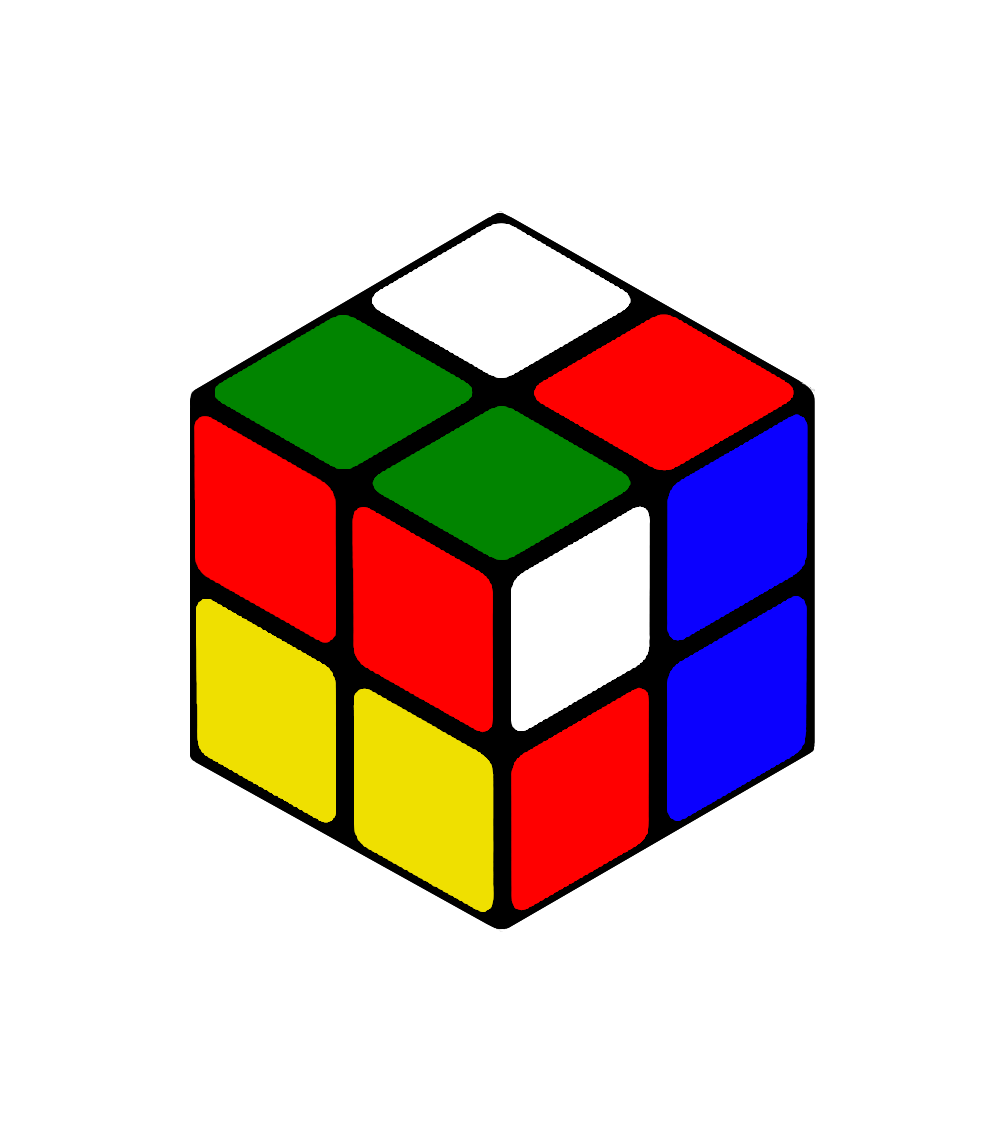
\includegraphics[scale=0.1]{RF.png}
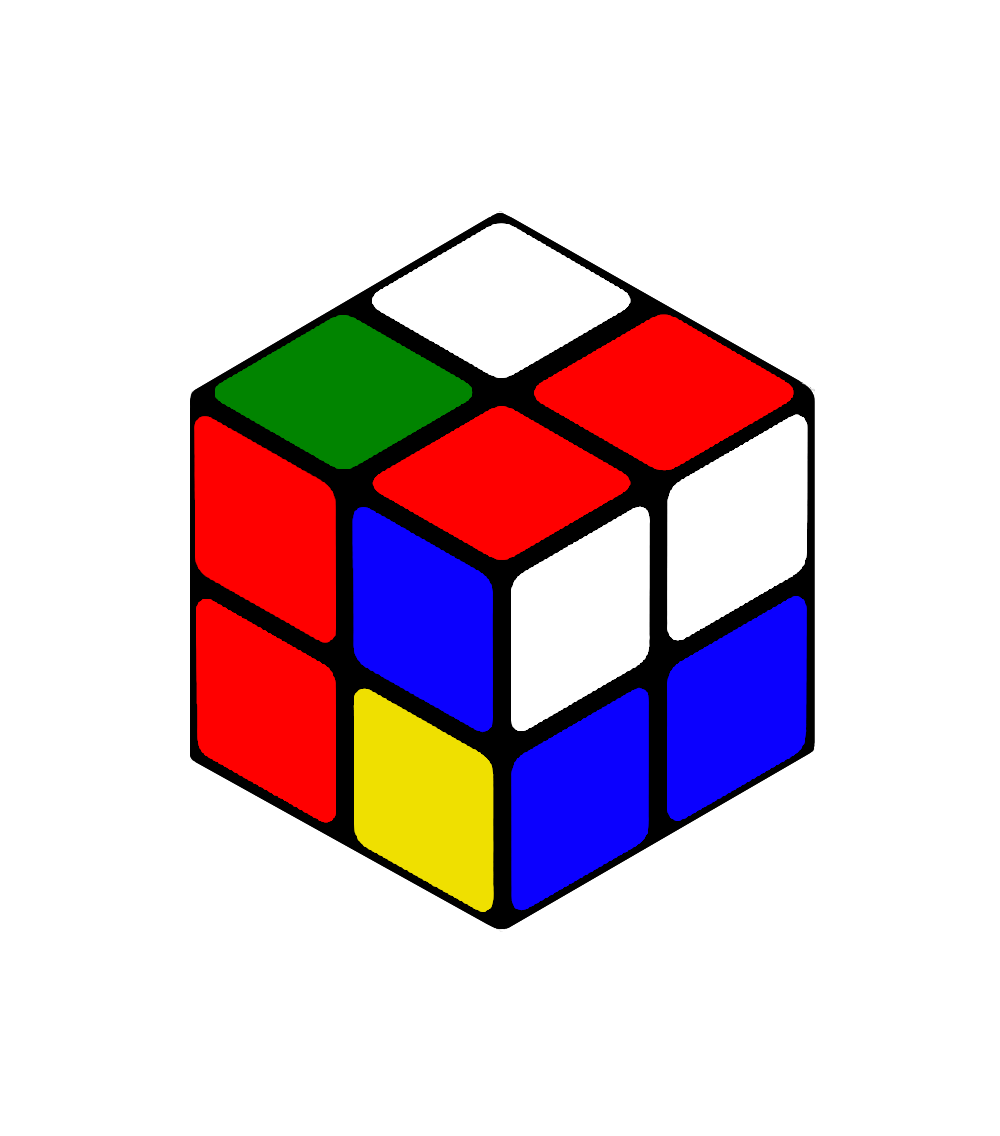
\includegraphics[scale=0.1]{FR.png}
\caption[Würfel nach Zügen $FR$ (links) und $RF$ (rechts)]{Würfel nach Zügen $FR$(links) und $RF$(rechts)}
\label{Abbildung_WürfelNachFRundRF}
\end{figure}
Außerdem wäre das Lösen des Würfels trivial, wenn die Kommutativität gelten würde.\cite{TD} Die Reihenfolge der gedrehten Ebenen wäre dann irrelevant und es müsste nur die Anzahl beachtet werden. 
Es gilt dementsprechend nicht $\forall \  Z_1, Z_2 \in \Gtwo. Z_1 \circ Z_2 = Z_2 \circ Z_1$ und der $\circ$-Operator der Gruppe ist somit nicht kommutativ. 

%
%
%
%
%
%
%
%
%
%
%=======================================================================================================
%
%
%
%
%
%
%
%
%
%
\subsection*{Züge als Gruppenoperation}\addcontentsline{toc}{subsection}{\protect\numberline{}Züge als Gruppenoperation}

Im Folgenden wird eine Gruppenoperation beschrieben, die eine Würfelkonfiguration durch das Ausführen eines Zuges auf eine neue Würfelkonfiguration abbildet. Bei Gruppenoperationen beeinflussen die Elemente einer Gruppe eine Menge. In diesem Fall beeinflussen die Züge des Würfels die Konfiguration des Würfels. Es handelt sich um eine Rechtsoperation, die im Kapitel \ref{Abschnitt_Gruppenoperation} beschrieben wurde.

Der Punktoperator ist definiert als $\cdot: M_C \times \Gtwo \rightarrow M_C$. Wenn der Zauberwürfel in einer Konfiguration $C=(\sigma, x)$ aus der Menge der Konfigurationen $M_C$ ist, wird er durch das Ausführen eines Zuges $Z \in \Gtwo$ in eine neue Konfiguration gebracht. Diese Konfiguration wird als $(C \cdot Z) \in M_C$ geschrieben.
Die folgenden beiden Eigenschaften müssen bei der Rechtsoperation gelten:

\begin{description}
\item [$\boldsymbol{C \cdot N = x}$ für alle $\boldsymbol{C \in M_C}$ und das neutrale Element $\boldsymbol{N \in \Gtwo}$] 
\ \\
Wenn der leeren Zug $N$ ausgeführt wird, wird die Konfiguration des Würfels nicht verändert. Daher gilt $C \cdot N = C$. 

\item [$\boldsymbol{C \cdot (Z_1 \circ Z_2) = (c \cdot Z_1) \cdot Z_2}$ für alle $\boldsymbol{Z_1, Z_2 \in \Gtwo}$ und $\boldsymbol{c \in M_C}$]
\ \\
Angenommen der Würfel befindet sich in der Konfiguration $C$. Wenn nun der Zug $Z_1 \in \Gtwo$ ausgeführt wird, ist die neue Konfiguration des Würfels $C \cdot Z_1$. Wenn nun noch ein weiterer Zug $Z_2 \in \Gtwo$ ausgeführt wird, ist die neue Konfiguration des Würfels $(C \cdot Z_1) \cdot Z_2$. 
Anders gesagt: Der Würfel hat in Konfiguration $C$ gestartet und der Zug $Z_1 Z_2$ wurde ausgeführt. Die neue Konfiguration kann auch als $C \cdot (Z_1 Z_2)$ geschrieben werden und somit gilt $(C \cdot Z_1) \cdot Z_2 = C \cdot (Z_1 Z_2)$. 
\end{description}

%
%
%
%
%
%
%
%=======================================================================================================
%
%
%
%
%

\subsection*{Ordnung der Permutationen}\addcontentsline{toc}{subsection}{\protect\numberline{}Ordnung der Züge} \label{Abschnitt_OrdnungPermutationen}
Wie bereits beschrieben, gilt $\forall Z \in \{ U, D, F, B, L, R \}, n \in \mathbb{N} \ . \ Z^n=Z^{n \mod 4}$, da alle Steine des Würfels in ihrer vorherigen Position bleiben, wenn eine Ebenen- oder eine Würfelrotation vier mal hintereinander ausgeführt wird. Dann werden die Züge $U, D, F, B, L, R$ als Züge der Ordnung 4 bezeichnet. 
Die Exponentenschreibweise kann für alle Züge aus $\Gtwo$ anwendet werden, auch wenn sie mehr als eine Ebene rotieren, beispielsweise bei $LLFF$. $(LLFF)^2$ entspricht dann $LLFFLLFF$ und $(LLFF)^3$ ist $LLFFLLFFLLFF$, was wieder die Ausgangsposition ergibt. 

Nicht nur die Züge $U, D, F, B, L, R$ kommen nach dem Wiederholen in den Ausgangszustand. Auch alle anderen Züge bringen den Würfel wieder in die Ausgangsposition des Zuges \cite{TD}. Es sind aber je nach Zug verschieden viele Wiederholungen nötig. Der Zug $(LLFF)$ hat beispielsweise die Ordnung 3, da der Würfel sich nach dreifacher Wiederholung von $(LLFF)$ wieder in der Ausgangsposition befindet. Es gilt dann $(LLFF)^3 = N$.
Weitere Beispielzüge mit Angabe der Ordnung sind: ${R^4= N}$ (Ordnung 4), ${(RRFF)^3 = N}$ (Ordnung 3) oder auch ${(LF)^{15}=N}$ (Ordnung 15). 
Die genannten Beispiele können an einem \Ttwo Würfel einfach ausprobiert werden.
Dabei muss beachtet werden, dass die Ordnung die Anzahl der Durchführungen beschreibt, die benötigt wird, damit alle Steine wieder an der Ausgangsposition sind. Die Ausrichtung der Steine wird hier aber nicht berücksichtigt. Es geht folglich nur um die Permutationen.


Im folgenden Abschnitt wird bewiesen, dass die Würfelsteine wieder in die Ausgangspositionen gelangen, wennn ein beliebiger Zug $Z \in \Gtwo$ wiederholt auf den Würfel anwendet wird.
Der folgende Beweis orientiert sich an dem Beweis aus \textit{Group Theory via Rubik's Cube} von Tom Davis \cite{TD}.

Jedes Mal wenn ein Zug wiederholt wird, werden die Steine im Würfel neu angeordnet. 
Da es eine endliche Anzahl an Würfelkonfigurationen gibt, muss eine Würfelposition wiederholt werden, wenn ein Zug oft genug durchführt wird.
Die Zahl der validen Würfelkonfigurationen ist zwar sehr groß, aber endlich ($11 \, 022 \, 480$). Demnach muss eine Position wiederholt werden, wenn der Zug öfter ausführt, als es mögliche Würfelpositionen gibt.

Bei einem beliebigen Zug $Z \in \Gtwo$ wird also irgendwann eine Würfelposition wiederholt. Wenn die wiederholende Würfelposition zuerst nach $n \in \mathbb{N}$ Wiederholungen auftritt und das zweite Mal nach $m \in \mathbb{N}$ Wiederholungen, sieht das so aus: $Z^n=Z^m$ mit $0 < n < m$.
Somit gilt dann $Z^{n-1} \neq Z^{m-1}$, da $m$ das zweite Vorkommen der gleichen Position repräsentiert.
Sonst wäre das erste Vorkommen der wiederholenden Positionen ja nach $n-1$ bzw. $m-1$ Wiederholungen.

Wenn $n=0$ wäre, ergibt das $Z^0=N$, was den leeren Zug (bzw. das neutrale Element) repräsentiert. Der Würfel wird dabei nicht verändert und somit wird die Würfelposition bei jedem Zug $Z \in \Gtwo$ mit $Z^0$ wiederholt. Deshalb müssen $n$ und $m$ größer als $0$ sein.

Wenn $Z^n = Z^m$ gilt, kommt der Würfel in die gleiche Endposition, wenn (auf die gleiche Ausgangsposition) $n$-mal oder $m$-mal $Z$ anwendet wird.
Wenn dann $Z^{-1}$ anwendet wird, ist die Endposition wieder gleich. Dabei ist es irrelevant, ob vorher $n$-mal oder $m$-mal $Z$ ausgeführt wurde, da von der gleichen Startposition ausgehend die gleiche Endposition erreicht wird, wenn der gleiche Zug ausführt wird.

Beim Anwenden von $Z^{-1}$ wird die letzte Ausführung von $Z$ wieder rückgängig gemacht. Wenn $Z$ $n$-mal ausgeführt wird und danach $Z^{-1}$ ausführt wird, ist es das gleiche wie $n-1$-mal $Z$ ausführen. Folglich gilt $Z^nZ^{-1}=Z^{n-1}$. Das gilt natürlich auch für $m$, also $Z^mZ^{-1}=Z^{m-1}$.
Demnach gilt dann $Z^{n-1}=Z^{m-1}$. Das widerspricht dann aber der Annahme, dass $m$ der kleinste Wert für eine Wiederholung der Position ist. Deshalb muss $n=0$ sein, damit $m$ die erste Wiederholung einer Position repräsentiert. 

Daraus folgt: Wenn ein Zug wiederholt auf einen Würfel anwendet wird, kommen die Steine wieder in die Ausgangsposition.
 
%
%
%
%
%
%
%
%
%
%
%=======================================================================================================
%
%
%
%
%
%
%
%
%
%


\subsection*{Zykelstruktur}\addcontentsline{toc}{subsection}{\protect\numberline{}Zykelstruktur}


Anhand der Zykelstruktur lässt sich die Ordnung des jeweiligen Zuges bestimmen. Die Ordnung beschreibt die Anzahl der Wiederholungen, die ein Zug durchgeführt werden muss, damit die Steine die gleiche Anordnung wie zu Beginn des Zuges haben. Dabei geht es um die Steinpositionen und nicht um die Steinausrichtungen.
Der Würfel kann demnach alle Steine an der richtigen Position haben und trotzdem ungelöst sein, da die Steine verdreht sein können. 

Der Zug $U$ als $\sigma_U =\ ( \ \textit{ulf} \ \textit{ulb} \ \textit{urb} \ \textit{urf} \ ) $ (eine Drehung der oberen Ebene um $90^\circ$ im Uhrzeigersinn) besteht aus einem 4-elementigen Zykel.
Wenn der Zug $U$ viermal ausgeführt wird, befindet sich der Würfel wieder in seiner vorherigen Position: 
\begin{center}
\begin{tabular}{ccccc}
\toprule
\textbf{Ausführung} & \textbf{ulf} & \textbf{ulb} & \textbf{urb} & \textbf{urf} \\
\midrule
1 & ulb & urb & urf & ulf \\

2 & urb & urf & ulf & ulb \\

3 & urf & ulf & ulb & urb \\

4 & ulf & ulb & urb & urf \\
\bottomrule
\end{tabular}
\end{center}

Die vierte Zeile der Tabelle hat die selbe Anordnung der Steine wie die oberste Zeile (vor Ausführung von $U$). 
Somit hat die beschriebene Ebenenrotation $U$ die Ordnung 4. Das gilt auch für jede andere Ebenenrotation ($D, F, B, L, R$).
Es gilt folglich für jeden Zug $Z$, der aus nur einem $n$-elementigen Zykel besteht: 
$\forall \ Z \in \Gtwo $ \textit{mit} $\sigma_Z=(i_1 \ i_2 \ ... \ i_n), n \in \mathbb{N} \ . \ { Z^n=N }$. \\
Wenn $Z$ mehrfach ausführt wird, wird nach jeder $n$-ten Wiederholung der Ausgangszustand erreicht. \cite{TD} 
Es gilt folglich auch 
$\forall \ Z \in \Gtwo $ \textit{mit} $ \ Z=(i_1 \ i_2 \ ... \ i_n), n,k \in \mathbb{N} \ . \  {Z^{k*n}=1 }$.
Auch bei komplexeren Zügen kann anhand der Zykelstruktur die Ordnung bestimmt werden. Dazu muss das kleinste gemeinsame Vielfache aller Zykelgrößen bestimmt werden. \cite{TD}

 
Der besseren Übersichtlichkeit halber, sind die Zykel aller Züge in Abbildung \ref{Abbildung_GraphAllerPermutationen} grafisch dargestellt.
Dieser Graph vereinfach das Ablesen der Zykel, wenn bei einem Zug mehrere Ebenenrotationen kombiniert werden.
\begin{figure}[H]
\centering
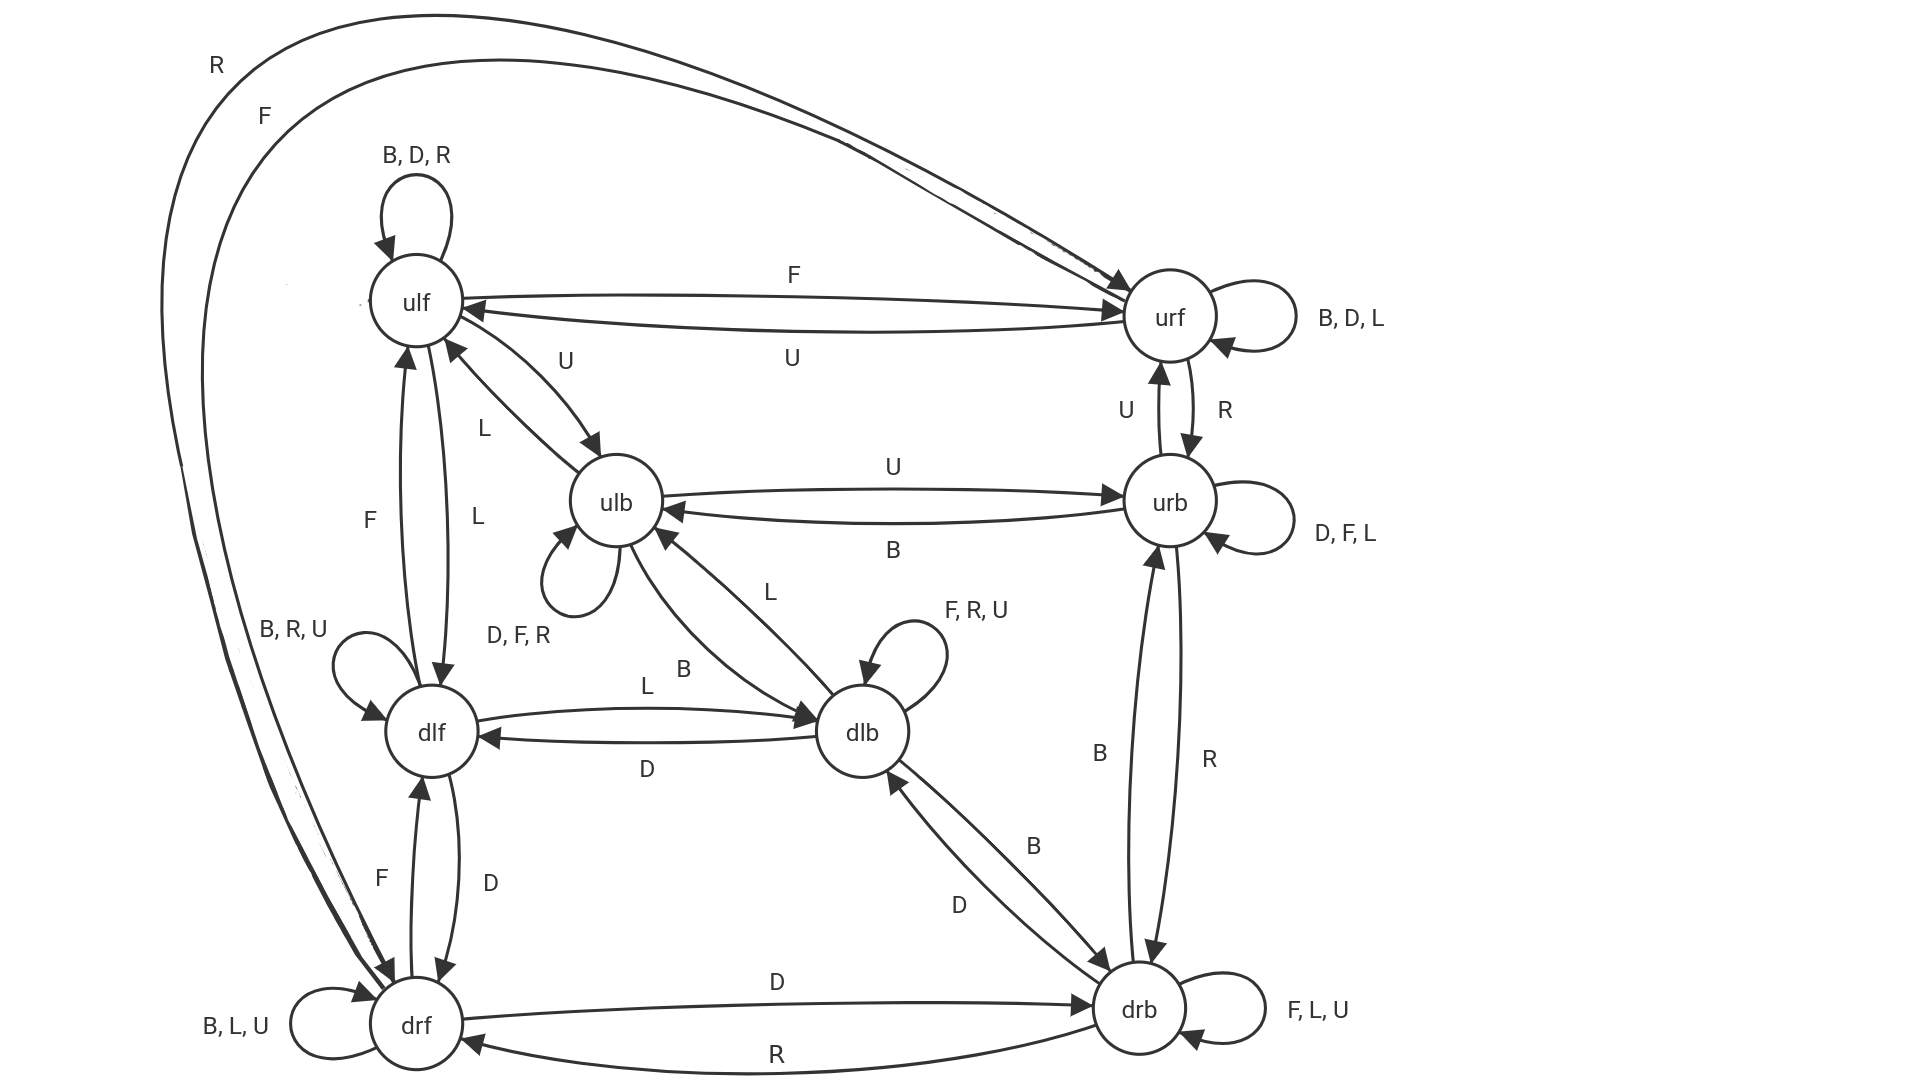
\includegraphics[scale=0.27]{graph_zug.png}
\caption[Graph aller Zugpermutationen]{Graph aller Zugpermutationen}
\label{Abbildung_GraphAllerPermutationen}
\end{figure}

So kann nun anhand des Beispielzuges $LLFF$ die Zykelstruktur dargestellt werden. 
Zuerst wird eine Tabelle erstellt, die jede Position auf ihre neue Position abbildet. Der Zug $LLFF$ setzt sich aus den Zügen $L$ und $F$ zusammen. 

\begin{center}
\begin{tabular}{ccccccccc}
\toprule
\textbf{Zug} & \textbf{ulb} & \textbf{urb} & \textbf{ulf} & \textbf{urf} & \textbf{dlb} & \textbf{drb} & \textbf{dlf} & \textbf{drf} \\
\midrule

L & ulf & \textcolor{gray}{urb} & dlf & \textcolor{gray}{urf} & ulb & \textcolor{gray}{drb} & dlb & \textcolor{gray}{drf} \\

L & dlf & \textcolor{gray}{urb} & dlb & \textcolor{gray}{urf} & ulf & \textcolor{gray}{drb} & ulb & \textcolor{gray}{drf} \\

F & ulf & \textcolor{gray}{urb} & \textcolor{gray}{dlb} & drf & urf & \textcolor{gray}{drb} & \textcolor{gray}{ulb} & dlf \\

F & urf & \textcolor{gray}{urb} & \textcolor{gray}{dlb} & dlf & drf & \textcolor{gray}{drb} & \textcolor{gray}{ulb} & ulf \\
\bottomrule
\end{tabular}
\end{center}

Die grauen Positionen bleiben bei der jeweiligen Ebenenrotation unverändert. 
Grafisch dargestellt sind die Zykel des Zuges $LLFF$ in Abbildung \ref{Abbildung_ZykelVonLLFF}. 
\begin{figure}[H]
\centering
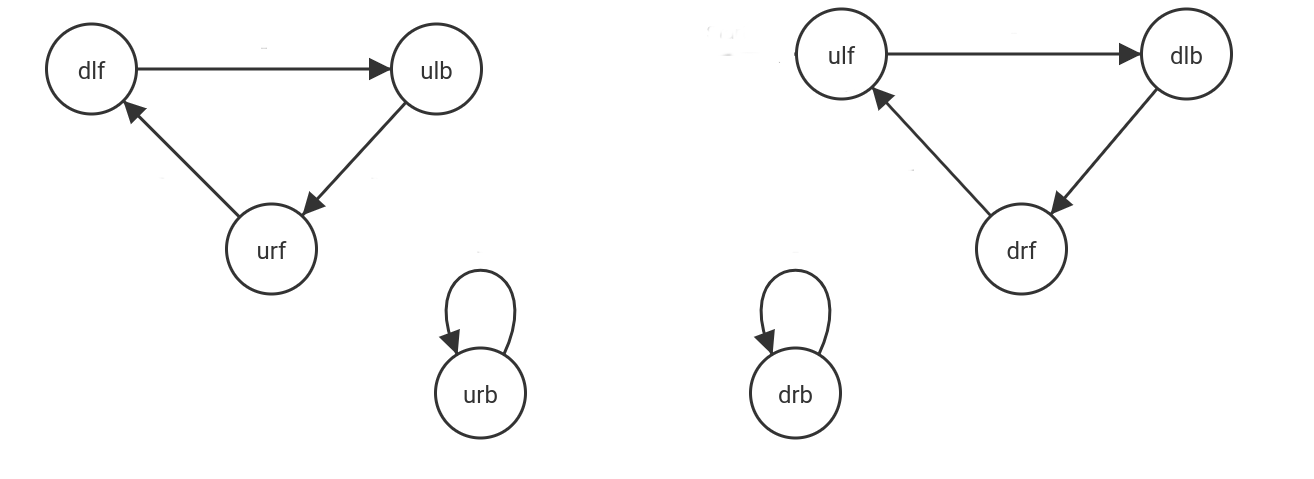
\includegraphics[scale=0.25]{zykel_LLFF.png}
\caption[Zykel des Zuges $LLFF$]{Zykel des Zuges $LLFF$}
\label{Abbildung_ZykelVonLLFF}
\end{figure}
In Zykelschreibeweise wird der Zug als $\sigma_{LLFF}=( \ \textit{dlf} \ \textit{ulb} \ \textit{urf})(\textit{ulf} \ \textit{dlb} \ \textit{drf} \ )$ geschrieben.
Da es demnach zwei Zykel der Länge drei gibt, befinden sich alle Würfelsteine nach drei Zügen ($KGV(3,3,1,1)=3$) wieder in ihrer Ausgangsposition. 
In diesem Fall sind die Steine nicht nur an der richtigen Position sondern auch so ausgerichtet, wie zu Beginn des Zuges. 
Außerdem ist zu sehen, dass sechs der acht Steine bei dem Zug $LLFF$ bewegt werden. Die anderen beiden (\textit{urb} und \textit{drb}) bleiben unverändert. 

%
%
%
%
%
%
%
%
%
%
%=======================================================================================================
%
%
%
%
%
%
%
%
%
%
%\subsection*{Äquivalenz von Zügen}\addcontentsline{toc}{subsection}{\protect\numberline{}Äquivalenz von Zügen}


%Es kann schwierig sein, die Äquivalenz von Zügen oder Roatationen anhand der Funktionen ($\sigma$ und $\delta$) in der Zykelschreibweise zu erkennen. 
%Das liegt daran, dass die Zykel in verschiedener Reihenfolge geschrieben werden können. So ist der Zug $U$ beispielsweise $ ( \ \textit{ulf} \ \textit{ulb} \ \textit{urb} \ \textit{urf} \ )$, aber auch $( \ \textit{urb} \ \textit{urf} \ \textit{ulf} \ \textit{ulb} \ )$.
%Um das zu vereinfachen, werden die Würfelpositionen priorisiert, so dass die Position mit der höchsten Priorität immer vorne steht und zwei Äquivalente Zykel somit gleich aussehen. 
%Die Positionen werden wie folgt priorisiert:
%\begin{center}
%\begin{tabular}{lcccccccc}
%Priorität & 1 & 2 & 3 & 4 & 5 & 6 & 7 & 8 \\
%\hline
%Position  & ulb & urb & ulf & urf & dlb & drb & dlf & drf \\
%\end{tabular}
%\end{center}
%Somit ist die angepasste Schreibweise für den Zug $U$ dann $( \ \textit{ulb} \ \textit{urb} \ \textit{urf} \ \textit{ulf} \ )$, da \textit{ulb} (falls vorhanden) ganz vorne stehen muss.

%
%
%
%
%
%
%
%
%
%
%=======================================================================================================
%
%
%
%
%
%
%
%
%
%
\newpage

\section{Untergruppen von G$_{2\times 2\times 2}$}

\label{Kapitel_Untergruppen}

Dieses Kapitel behandelt die Untergruppen von $(\Gtwo, \circ)$. Im ersten Teil wird auf die trivialen Untergruppen eingegangen. Außerdem werden noch weitere Untergruppen beschrieben und erzeugt.
Die Definition und Erklärung der Untergruppe und des Erzeugers findet sich in Kapitel \ref{Abschnitt_Untergruppe}.
Außerdem werden die Cayleygraphen zu zwei Untergruppen dargestellt und erklärt.

%
%
%
%
%
%
%
%
%
%
%=======================================================================================================
%
%
%
%
%
%
%
%
%
%
\subsection*{Untergruppen Beispiele}\addcontentsline{toc}{subsection}{\protect\numberline{}Untergruppen Beispiele}



Jede Gruppe G mit neutralem Element $N$ hat die beiden trivialen Untergruppen ${H_N = \{N\}}$ und $H_G=G$ (hier: $G=\Gtwo$). Demnach sind $H_N$ und $H_G$ die trivialen Untergruppen von $\Gtwo$ ($H_N \leqslant \Gtwo$ und $H_G \leqslant \Gtwo$).
Die Gruppe $\Gtwo$ hat viele Untergruppen, deshalb kann hier nur auf einen Teil davon erwähnt werden. 


Da die trivialen Untergruppen nicht sonderlich aussagekräftig sind, geht der folgende Abschnitt auf einige anschauliche Untergruppen zum Lösen des Würfels ein. Diese Gruppen hat Tom Davis (in  \textit{Group Theory via Rubik's Cube}) \cite{TD} für den 3x3x3-Würfel genannt. Hier werden zwei seiner Untergruppen auf den 2x2x2 übertragen: 
\begin{itemize}
\item Die Untergruppe $H_{E1}$, die nur die Rotation einer Ebene zulässt, hat nur vier erreichbare Würfelkonfigurationen (sowohl beim 2x2x2- als auch beim 3x3x3-Würfel). Das kann auch gut an einem \textit{Cube} nachvollzogen werden, da durch das Drehen von nur einer Ebene auch nur vier verschiedene Ergebnisse erzielt werden können.
\item Eine weitere Untergruppe von $\Gtwo$ ist $H_{E2}$. Hier dürfen zwei gegenüberliegende Ebenen gedreht werden. 
Bei der Gruppe des \Tthree Würfels ergeben sich daraus 16 mögliche Würfelkonfigurationen \cite{TD}. Bei dem \Ttwo \textit{Cube} allerdings nur vier, da es nur zwei Ebenen gibt und nicht anhand der Mittelsteine oben und unten unterschieden werden kann.
\end{itemize}


%
%
%
%
%
%
%
%
%
%
%=======================================================================================================
%
%
%
%
%
%
%
%
%
%

\subsection*{Erzeuger}\addcontentsline{toc}{subsection}{\protect\numberline{}Erzeuger}

Die folgenden Beispiele stammen aus Tom Davis' \textit{Group Theory via Rubik's Cube} \cite{TD} und werden hier von der Gruppe des \Tthree \textit{Cubes} auf den \Ttwo \textit{Cube} übertragen.


Ein Beispiel eines Erzeugers einer Untergruppe $F$ von $(\Gtwo, \circ)$ wird von $\{ F \}$ erzeugt. Es können nur $4$ Würfelkonfigurationen erreicht werden und die $F$ enthält somit nur die Elemente ${N, F, FF, FFF}$, da alle weiteren Züge äquivalent zu einem dieser Züge sind. $FFFF$ ist das gleiche wie das neutrale Element $N$ und der Würfel bleibt in der Ausgangsposition.


Ein weitere Beispiel ist die Untergruppe, die von $\{FF\}$ erzeugt wird. Dabei können die Ebenen nur halbe Drehungen (statt Vierteldrehungen) machen und somit nur zwei Positionen erreichen. Die Untergruppe enthält daher nur $FF$ und $FFFF$.


Die komplette Gruppe $(\Gtwo, \circ)$ wird erzeugt durch $\{U, D, R, L, F, B\}$.

Die Untergruppen, die mit nur einem Element aus $\Gtwo$ erzeugt werden, sind zyklische Gruppen. Die oben beschriebene Untergruppe $F$, die durch $\langle F \rangle$ erzeugt wird, ist somit eine zyklische Untergruppe.
Die Untergruppe $F$ wird erzeugt durch $\langle F \rangle = \{ F^n \mid n \in \mathbb{Z}\}$. Das bedeutet, dass $F = \{N, F^1, F^2, F^3, F^4, ...\}$. Es gibt auch unendliche zyklische Gruppen, diese hier sind aber endlich, da $N = FFFF$. Die Züge werden (wie bereits in Kapitel \ref{Kapitel_WürfelAlsGruppe} beschrieben) modulo $4$ gerechnet.
Das gilt für jeden Erzeuger, der nur aus einer einzelnen Ebenendrehung besteht.


Da die Gruppe $(\Gtwo, \circ)$ endlich ist, erzeugt jedes Element der Gruppe eine endliche zyklische Untergruppe \cite{TD}. Die Größe dieser Untergruppe hängt von der Ordnung des Zuges ab. Die Ordnung wurde in Kapitel \ref{Abschnitt_OrdnungPermutationen} beschrieben.
Die Ordnung des Zuges $FR$ ist 15 -- wenn $FR$ 15-mal auf dem \Ttwo Würfel ausführt wird, ist er wieder in der Ausgangsposition. Bei dem \Tthree Würfel ist die Ordnung des Zuges $FR$ allerdings 105 \cite{TD}.
Die Gruppe, die durch $\{FR\}$ erzeugt wird, hat somit 15 Elemente.
%
%
%
%
%
%
%
%
%
%=======================================================================================================
%
%
%
%
%
%
%
%
%
%

\subsection*{Durch \textit{FF} und \textit{RR} erzeugte Untergruppe}\addcontentsline{toc}{subsection}{\protect\numberline{}Durch $FF$ und $RR$ erzeugte Untergruppe}

Das Beispiel der durch $\{ FF, RR \}$ erzeugten Untergruppe hat Tom Davis auch gewählt \cite{TD} und hier wird es von dem \Tthree \ auf den \Ttwo Würfel übertragen.
Da die beiden Züge als Einheiten gesehen werden, muss jede der Ebenendrehungen eine halbe Drehung sein.
Es wurde in Kapitel \ref{Kapitel_WürfelAlsGruppe} bereits gezeigt, dass $(FF)^2 = N$ und $(RR)^2 = N$ gilt, da der Würfel dann wieder in der Ausgangsposition ist.

Wenn bei einen gelösten \Ttwo Würfel $FFRR$ ausführt wird, befindet sich der Würfel nach 3 Wiederholungen wieder in der Startkonfiguration. Das gilt auch für den Zug $RRFF$. Die Ordnung von $FFRR$ und $RRFF$ ist daher 3. Bei dem \Tthree \textit{Cube} ist die Ordnung dieser Züge 6 \cite{TD}.

Die durch $\{ FF, RR \}$ erzeugte Untergruppe des \Tthree Würfels hat somit auch mehr Elemente als die des \Ttwo Würfels. Theoretisch sind das alle Mitglieder der Untergruppe des \Ttwo \textit{Cubes}, wenn dabei berücksichtigt wird, dass $FFFF$ und $RRRR$ keine Veränderung ergeben: $N$, $FF$, $RR$, $FFRR$, $RRFF$, $FFRRFF$, $FFRRFF$, $(FFRR)^2$, $(RRFF)^2$, $FF(RRFF)^2$, $RR(FFRR)^2$, $(FFRR)^2FF$ und $(RRFF)^2RR$. 
Wenn diese Züge an einem Würfel ausprobiert werden, stellt sich aber heraus, dass beispielsweise $(RRFF)^2RR$ bei gleichem Startzustand die gleiche Würfelkonfiguration wie $FF$ ergibt. Wenn diese Doppelungen aussortiert werden, verbleiben folgende sieben Gruppenelemente:
\begin{center}
\centering
\begin{tabular}{c c c c}
$N$ & $RR$ & $FFRR$ &  $RRFFRR$ \\
& $FF$ & $RRFF$ & $FFRRFF$   \\
\end{tabular}
\end{center}
Zum Vergleich: Tom Davis kommt bei dem  \Tthree Würfel auf zwölf Elemente in der durch $\{ FF, RR \}$ erzeugten Untergruppe.

Die doppelten Elemente können natürlich auch mathematisch erkannt werden, dafür müssen dann nicht alle Optionen an einem Würfel ausprobiert werden.
Das wird im Folgenden beispielhaft mit $(RRFF)^2RR$ gemacht. Das ist ausgeschrieben $RRFFRRFFRR$. Da $RRFF$ die Ordnung 3 hat, befindet sich der Würfel nach $(RRFF)^3 = RRFFRRFFRRFF$ wieder in der Ausgangsposition. Daraus kann geschlossen werden, dass von dem Zug $RRFFRRFFRR$ aus nur noch $FF$ bis zur Ausgangsposition fehlt und dass (da es sich um halbe Drehungen handelt) die Position, die durch $RRFFRRFFRR$ erreicht wird auch durch $FF$ erreichbar ist.

Die Tatsache, dass $\{ FF, RR \}$ eine Untergruppen mit nur 7 bzw. 12 Elementen bei dem \Ttwo \  bzw. dem \Tthree Würfel erzeugt, ist besonders überraschend, da $\{ F, R \}$ bei dem  \Tthree Würfel eine Untergruppe der Größe $73\, 483\, 200$ erzeugt \cite{TD}. 
Bei dem \Ttwo \textit{Cube} kommt die Untergruppe mit $120 \cdot 3^5$ auf $29 \, 160$ Mitglieder, aber auch das ist deutlich größer als $7$.

%
%
%
%
%
%
%
%=======================================================================================================
%
%
%
%
%
%
%
%
%

\subsection*{Cayleygraph}\addcontentsline{toc}{subsection}{\protect\numberline{}Cayleygraph}
Cayleygraphen wurden in Kapitel \ref{Abschnitt_Cayleygraph} eingeführt. Sie dienen der Visualisierung von Untergruppen und deren Erzeugern.

\begin{figure}[H]
\centering
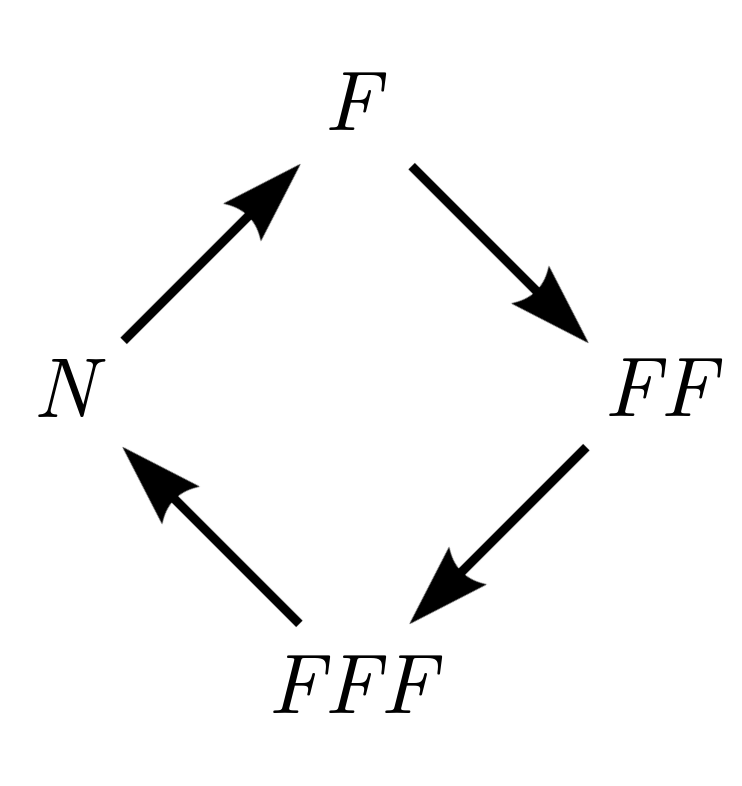
\includegraphics[scale=0.6]{Cayleygraph1.png}
\caption{Cayleygraph zu Erzeuger $\{ F \}$}
\label{Abbildung_CayleygraphF}
\end{figure}

Ein simples Beispiel ist in Abbildung \ref{Abbildung_CayleygraphF} zu sehen: Der Cayleygraph der Untergruppe $F$ von $(\Gtwo, \circ)$, die durch $\{ F \}$  erzeugt wird.
Dieser Cayleygraph ist anschaulich, der er nicht sonderlich komplex ist.
Die Untergruppe wird durch die Ebenendrehung $F$ erzeugt, daraus ergibt sich durch hinzufügen einer weiteren Drehung der vorderen Ebene um $90^\circ$ dann $FF$, dann $FFF$ und dann $FFFF$, was dem neutralen Element $F$ entspricht.


Der Cayleygraph der durch $\{ FF, RR \}$ erzeugten Untergruppe ist etwas komplexer (s. Abbildung \ref{Abbildung_CayleygraphFFRR}). 
Die roten Pfeile repräsentieren den Erzeuger $\{FF\}$ (da es sich dabei in der Startkonfiguration um die rote Seite des Würfels handelt) und die blauen Pfeile repräsentieren den Erzeuger $\{RR\}$ (da es sich dabei um die blaue Würfelseite handelt).
Elemente die durch ein anderes Element in Kombination mit einem Erzeuger entstehen können, sind durch einen Pfeil (Erzeuger) miteinander verbunden.
Die 7 Elemente der durch  $\{ FF, RR \}$ erzeugten Untergruppe sind die Knoten des Graphens. 
Anhand des Cayleygraphens ist zu sehen, dass $FFFF$ und $RRRR$ das neutrale Element $N$ ergeben.
Obwohl dieser Cayleygraph wesentlich komplexer ist, als der der Untergruppe $F$ (Abbildung \ref{Abbildung_CayleygraphF}), stellt er eine sehr kleine erzeugte Untergruppe dar, wenn es mit der Größe der anderen erzeugbaren Untergruppen von $(\Gtwo, \circ)$ verglichen wird. Die Untergruppen und Cayleygraphen können bei der Gruppe des \Ttwo Würfels (und des \Tthree Würfels) sehr groß werden.

\begin{figure}[H]
\centering
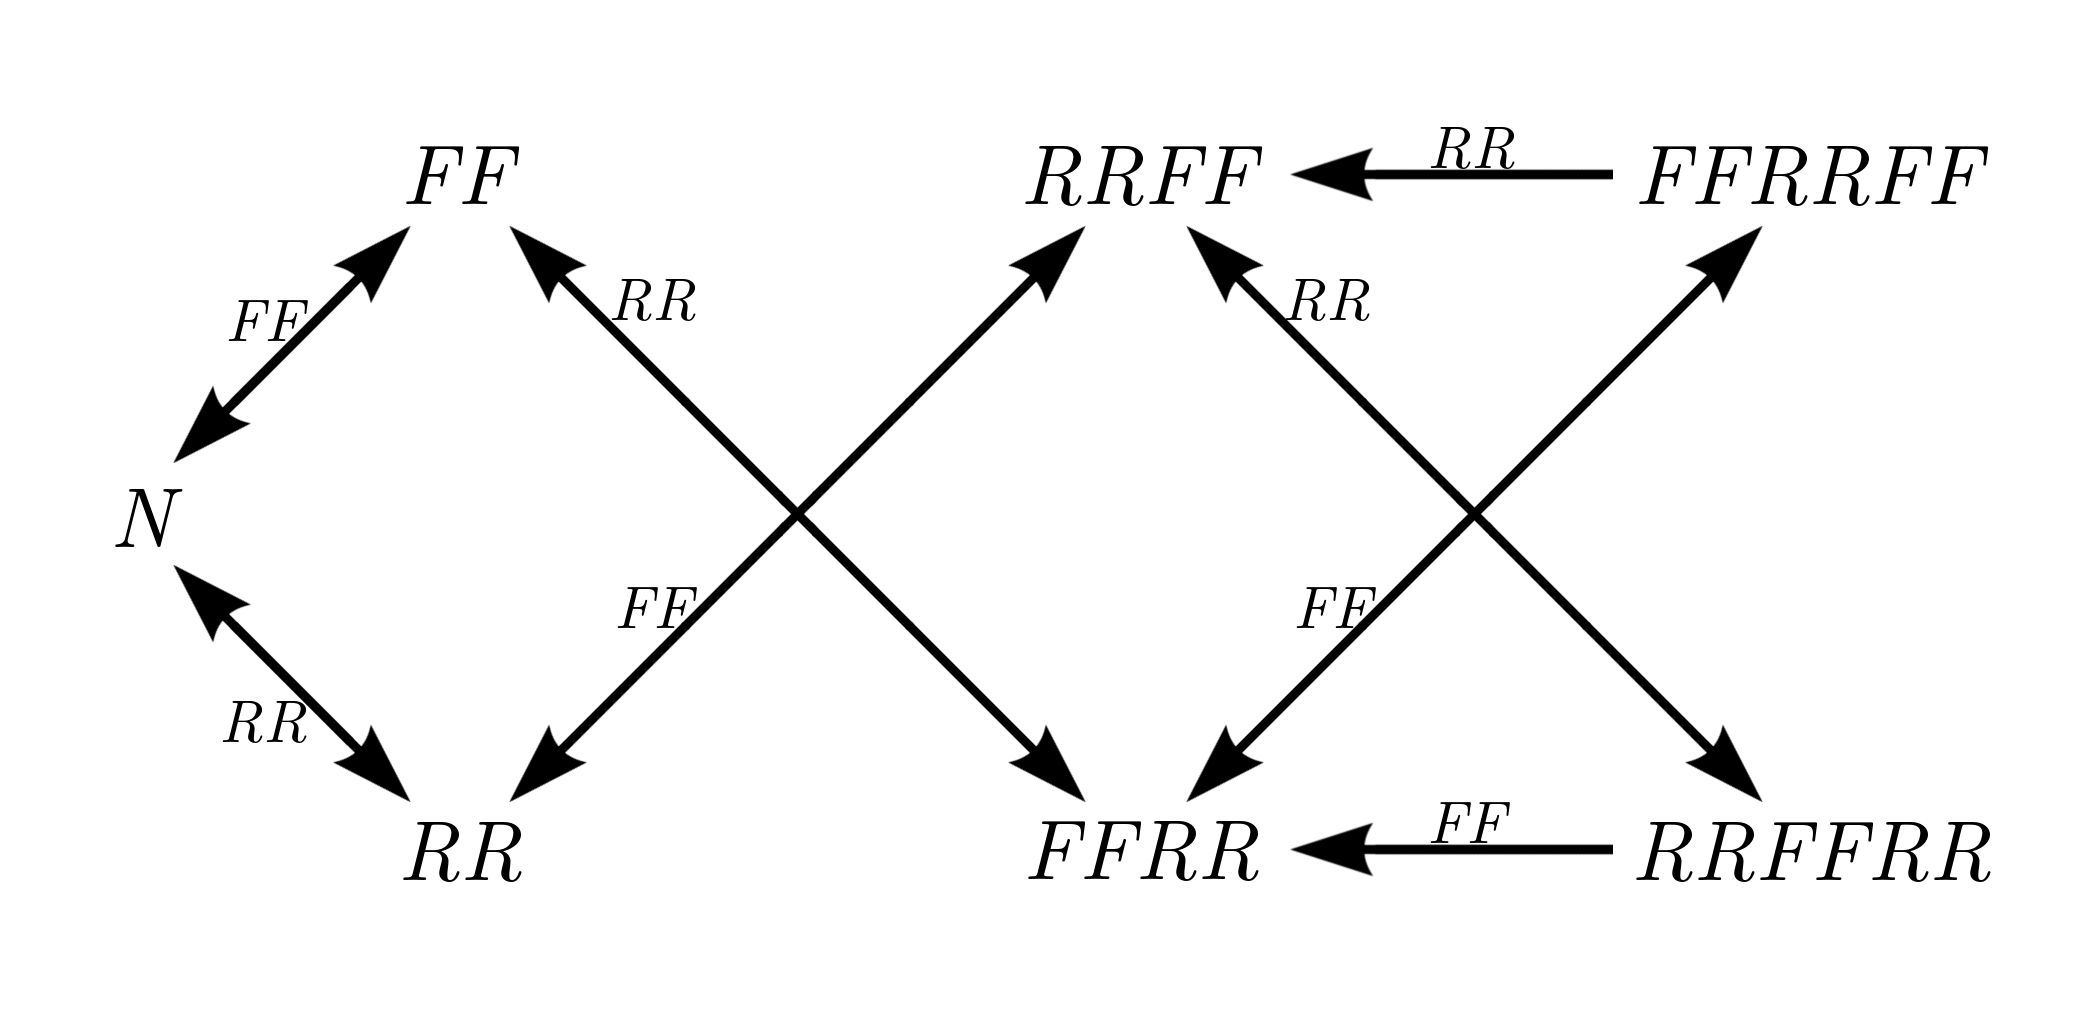
\includegraphics[scale=0.65]{Cayleygraph2.png}
\caption{Cayleygraph zu Erzeuger $\{ FF, RR \}$}
\label{Abbildung_CayleygraphFFRR}
\end{figure}







%
%
%
%
%
%
%
%=======================================================================================================
%
%
%
%
%
%
%
%
%
%
\newpage

\section{Valide Konfigurationen des Würfels}

\label{Kapitel_ValideKonfigurationen}

In diesem Kapitel wird Anzahl der validen Würfelkonfiguratione berechnet -- sowohl anhand des Würfels als auch mithilfe der Gruppe $(\Gtwo,\circ)$. Dazu wird die Mächtigkeit der Gruppe berechnet. Die Definition der Mächtigkeit und Beispiele sind in Kapitel \ref{Abschnitt_MächtigkeitGruppe} zu finden. Es wird auch die theoretische Obergrenze der möglichen Würfelkonfigurationen berechnet. \\
Außerdem wird gezeigt, dass für die Ausrichtung $x$ der Steine $( \sum_{i= 1}^{8} \ x_i ) \mod 3 = 0$ gilt.

%
%
%
%
%
%
%
%
%
%=======================================================================================================
%
%
%
%
%
%
%
%
%
%
\subsection*{Anzahl der validen Würfelkonfigurationen}\addcontentsline{toc}{subsection}{\protect\numberline{}Anzahl der validen Würfelkonfigurationen}
\label{Abschnitt_AnzahlKonfigurationen}

Im Folgenden wird die Anzahl der möglichen Würfelkonfigurationen brechnet. Nicht jede der theoretisch möglichen Würfelkonfigurationen kann auch wirklich durch Ebenendrehungen erreicht werden. Wie viele Möglichkeiten es im \Ttwo Würfel gibt und welche davon wirklich erreichbar sind, wird nun schrittweise anhand des Würfelaufbaus berechnet. \\
Dazu wird zuerst die Anzahl der theoretisch möglichen Würfelkonfigurationen berechnet:
Die Ecksteine können sich in jeder der acht Ecken befinden. Deshalb gibt es pro Eckstein 8 mögliche Positionen im Würfel. Da es 8 Ecksteine gibt, gibt es somit $8! = 1 \cdot 2 \cdot 3 \cdot 4 \cdot 5 \cdot 6 \cdot 7 \cdot 8 = 40\, 320$ mögliche Positionen für die Ecksteine. \\
Außerdem können die Ecksteine gedreht sein, es können also verschiedene Farbflächen oben sein. Da die Steine aus 3 Farbflächen bestehen, können sieben davon durch Ebenendrehungen theoretisch 3 verschiedene Ausrichtungen annehmen. Der achte Stein kann durch die Möglichkeit der Rotation des kompletten Würfels als richtig gedreht angenommen werden. Es gibt folglich $3^7 = 2187$ Wege, wie die Ecksteine ausgerichtet sein können.
Da es keine Mittelsteine im Würfel gibt, reduziert die Rotation des Würfels die Möglichkeiten um den Faktor 24, denn es gibt $6$ Seiten, die jeweils $4$ Ausrichtungen haben können. Das sind dann $6 \cdot 4 = 24$.
Somit ergibt es $(3^7 \cdot 8!) \cdot \frac{1}{24}$ mögliche Positionen für den Würfel. Das sind $3\, 674\, 160$ Positionen.

Die theoretische Obergrenze der Würfelkonfigurationen liegt bei $8! \cdot 3^8 = 264 \, 539 \, 520$ \cite{MMFAA}. Davon sind aber nicht alle Rotationen durch Ebenedrehungen erreichbar und die Rotationen des Würfels wurden auch nicht berücksichtigt.


%
%
%
%
%
%
%
%
%
%=======================================================================================================
%
%
%
%
%
%
%
%
%
%
\newpage
\subsection*{Mächtigkeit von G$_{2\times 2\times 2}$}\addcontentsline{toc}{subsection}{\protect\numberline{}Mächtigkeit von G$_{2\times 2\times 2}$}

Die Mächtigkeit der Gruppe $(\Gtwo,\circ)$ (bzw. $|\Gtwo|$) ist die Anzahl der Elemente von $\Gtwo$. Die Mächtigkeit der Gruppe ist die Anzahl der validen Würfelkonfigurationen, da die $\Gtwo$ die Äquivalenzklassen aller möglichen Züge enthält. Wenn zwei Züge mit gleicher Ausgangskonfiguration die gleiche Folgekonfiguration des Würfels hervorrufen, sind sie Repräsentanten der gleichen Äquivalenzklasse in $\Gtwo$. Somit bringt Element von $\Gtwo$ den Würfel in eine andere Würfelkonfiguration und es sind keine äquivalenten Züge doppelt enhalten. Außerdem wurden die Äuivalenzklassen mit der Menge alle Züge des Würfels gebildet. Somit ist jeder mögliche Zug enthalten und $|\Gtwo|$ ist die Anzahl der validen Würfelkonfigurationen.

Da Mächtigkeit der Gruppe $(\Gtwo,\circ)$ der Anzahl der validen Würfelkonfigurationen entspricht, setzt sie sich aus dem Produkt der Konfigurationsparameter $\sigma$ und $x$ zusammen. Daraufhin müssen aber auch die Äquivalenzen bezüglich der Rotationen des Würfels berücksichtigt werden.

$\sigma$ ist die Menge der bijektiven Funktionen für jede Ebenenrotation. Es sind die Übergänge der acht Würfelsteine als Permutationen enthalten. Da es $8$ Permutationsobjekte gibt, ist die Anzahl der Permutationsmöglichkeiten $8! = 40320$.

Der andere Parameter der Würfelkonfiguration ist der 8-dimensionale Vektor $x$. Jeder der Werte in $x$ ist aus der Menge $\{0,1,2\}$. Somit gibt es drei Möglichkeiten für jeden Wert im Vektor. Das ergibt dann $3^8 = 6561$ mögliche Konfigurationen des Vektors.

Ohne Berücksichtigung der Äquivalenzklassen wird ein Wert von $40320 \cdot 6561 = 264 \, 539 \, 520$ möglichen Konfigurationen erreicht. Da durch die Rotationen eine der Steinausrichtungen in $x$ als richtig angenommen werden kann, wird $264 \, 539 \, 520$ durch drei geteilt und ergibt dann $88 \, 179 \, 840$. 
Außerdem gibt es bei den Rotationen sechs Rotationsmöglichkeiten (und zusätlich die \textit{leere} Rotation). Jede dieser Rotationsmöglichkeiten kann vier verschiedene Rotationen hervorrufen. Das ergibt dann $6 \cdot 4 = 24$ Möglichkeiten, die in den Äquivalenzklassen berücksichtigt werden. Somit muss $88 \, 179 \, 840$ durch $24$ geteilt werden, um die Mächtigkeit der Gruppe $(\Gtwo,\circ)$ zu berechnen. $|\Gtwo|$ ist dann $88 \, 179 \, 840 \div 24 = 3\, 674\, 160$.

Die Mächtigkeit der Gruppe $(\Gtwo,\circ)$ ist also die Anzahl der validen Würfelkonfigurationen $3\, 674\, 160$.


%Das wird nun anhand der Gruppe $(\Gtwo,\circ)$ berechnet. Die Gruppe ist eine symmetrische Gruppe (s. Kapitel \ref{Abschnitt_SymmetrischeGruppe}), da sie aus allen Permutationen der $8$-elementigen Menge $\{ \textit{ulb},  \textit{urb},  \textit{ulf},  \textit{urf},  \textit{dlb},  \textit{drb},  \textit{dlf},  \textit{drf} \}$ besteht. Dadurch ist die Mächtigkeit dieser Gruppe $|\Gtwo| = 8!=40\, 320$. \\
%Es müssen aber auch die Äquivalenzrelationen der Rotationen von $(\Gtwo,\circ)$ berücksichtigt werden. Es gibt die Äquivalenzrelationen $\{{Z_r}, {Z_l}, {Y_r}, {Y_l}, {X_r}, {X_l}, N\}$ -- die Rotation um die Achsen $X, Y$ und $Z$, jeweils nach rechts und links. Da zwei Linksdrehungen und zwei Rechtsdrehungen äquivalent sind, gibt es demnach für jede Achse vier Rotationsmöglichkeiten. Das sind dann $3 \cdot 4 = 12$ Rotationen. Da aber zu jeder Achse zwei Seiten gehören, die getauscht werden können, sind es $2 \cdot 12 = 24$ Rotationen.
%Die Mächtigkeit der Gruppe ($40\, 320$) muss aufgrund der Rotationsmöglichkeiten um den Faktor $24$ reduziert werden, wenn die Anzahl der validen Würfelkonfigurationen anhand der Gruppe berechnet werden soll. Das sind dann $40\, 320 \cdot \frac{1}{24} = 1680$ mögliche Positionen der Ecksteine unter Berücksichtigung der Würfelrotationen. Diese Zahl scheint verhältnismäßig niedrig, da die Ausrichtung der Steine noch nicht berücksichtigt wurde. \\
%Die Ausrichtung der Steine wird durch den $8$-dimensionalen Vektor $x$ dargestellt. Jeder Eintrag in $x$ kann die Werte $0, 1$ oder $2$ annehmen. Das ergibt $3^8=6561$ Möglichkeiten der Steinausrichtung. Allerdings kann durch die Äquivalenzrelationen (bzw. die Rotation des Würfels) einer der Steine als richtig angenommen werden. Das ergibt dann $3^7=2187$ Möglichkeiten der Steinausrichtung. Somit gibt es $40\, 320 \cdot \frac{1}{24} \cdot 2187 = 3\, 674\, 160$ valide Würfelkonfigurationen. Da die Gruppe $(\Gtwo,\circ)$ allerdings nur die Position der Steine berücksichtig, ist die Mächtigkeit $|\Gtwo| = 40\, 320$.




%
%
%
%
%
%
%
%
%
%
%=======================================================================================================
%
%
%
%
%
%
%
%
%
%
\subsection*{Ausrichtung der Steine (modulo 3)}\addcontentsline{toc}{subsection}{\protect\numberline{}Ausrichtung der Steine (modulo 3)}

Die Konfiguration des Würfels ist definiert als $C=(\sigma, x)$. In diesem Abschnitt wird gezeigt, dass bei einer validen Würfelkonfiguration \begin{displaymath}
\left( \sum_{i= 1}^{8} \ x_i \right) \hspace*{-0.7em} \mod 3 = 0 
\end{displaymath}  (modulo) gilt. 

Wenn $C'=(\sigma', x')$ eine Nachfolgekonfiguration von der Konfiguration $C=(\sigma, x)$ ist, dann gilt  ${(\sigma, x) \cdot M = (\sigma', x')}$. Dabei ist $M$ eine der Züge aus $U, D, R, L, F, B$. Es gilt dann ${(\sum_{i= 1}^{8} \ x_i') \mod 3 = (\sum_{i= 1}^{8} \  x_i) \mod 3 }$.

In Abbildung \ref{Abbildung_XnachZugR} in Kapitel \ref{Abschnitt_AusrichtungDerSteine} ist diese Situation für den Zug $R$ dargestellt. Das kann auch in dieser Tabelle gesehen werden: 
\vspace*{1em}

\begin{adjustbox}{width=1\textwidth,center}

\begin{tabular}{cllcc}
\toprule
 \textbf{Zug} $\boldsymbol{M}$ & \hspace*{2.2cm}$\boldsymbol{x}$ & \hspace*{2cm} $\boldsymbol{x'}$ &  $\boldsymbol{\sum_{i= 1}^{8} x_i'} \ \ \ $ & $\boldsymbol{\mod 3}$ \\
\midrule
\textit{D} & $(x_1, x_2, x_3, x_4, x_5, x_6, x_7, x_8)$ & $(x_1, x_2, x_3, x_4, x_6, x_8, x_5, x_7)$ & 0 & 0 \\

\textit{U} & $(x_1, x_2, x_3, x_4, x_5, x_6, x_7, x_8)$ & $(x_3, x_1, x_4, x_2, x_5, x_6, x_7, x_8)$ & 0 & 0 \\

\textit{R} & $(x_1, x_2, x_3, x_4, x_5, x_6, x_7, x_8)$ & $(x_1, 2, x_3, 1, x_5, 1, x_7, 2)$ & 6 & 0 \\

\textit{L} & $(x_1, x_2, x_3, x_4, x_5, x_6, x_7, x_8)$ & $(1, x_2, 2, x_4, 2, x_6, 1, x_8)$ & 6 & 0 \\

\textit{F} & $(x_1, x_2, x_3, x_4, x_5, x_6, x_7, x_8)$ & $(x_1, x_2, 1, 2, x_5, x_6, 2, 1)$ & 6 & 0 \\

\textit{B} & $(x_1, x_2, x_3, x_4, x_5, x_6, x_7, x_8)$ & $(2, 1, x_3, x_4, 1, 2, x_7, x_8)$ & 6 & 0 \\
\bottomrule

\end{tabular}

\end{adjustbox}

\ \\
Für jede valide Würfelposition gilt folglich ${(\sum_{i = 1}^{8} \ x_i') \mod 3 = (\sum_{i = 1}^{8} \  x_i) \mod 3 }$. 
Wenn es eine valide Konfiguration $C'=(\sigma', x')$, für die gilt $\sum_{i = 1}^{8} x_i' \mod 3 = 0$, dann gibt es einen Zug $M \in \Gtwo$, so dass $M \cdot C'$ die Steine in die Konfiguration $(1,x)$ bringt Alle Steine befinden sich dann an der richtigen Position, sind aber nicht korrekt ausgerichtet. 
Von dieser Konfiguration $(1,x)$ ausgehend gibt es einen Zug $M \in \Gtwo$, so dass alle Eckstücke richtig ausgerichtet sind. Dann ergibt sich die Konfiguration $(1, 0)$ und alle Eckstücke sind in der richtigen Ausrichtung und Position. Der Würfel befindet sich dann in der Startkonfiguration. 
%
%
%
%
%
%
%
%
%
%
%=======================================================================================================
%
%
%
%
%
%
%
%
%
%
\newpage


\section{Lösung des Würfels}

\label{Kapitel_Lösung}

Die übliche, händische Methode zum Lösen eines Zauberwürfels ist das Kombinieren verschiedener Ebenendrehungen. Diese werden als eine Einheit angewendet und verändern den Würfel dann sehr spezifisch. 
Es gibt beispielsweise eine Kombination, die 3 der 4 Ecken der oberen Ebene untereinander im Uhrzeigersinn tauscht und deren Ausrichtung dabei nicht verändert. 

In diesem Kapitel wird die Parität der Züge beschrieben und Kommutatoren erklärt.
Dann wird beispielhaft ein Lösungsvorgang eines Menschens schrittweise beschrieben und erklärt.
Außerdem werden Muster des Würfels algorithmisch beschrieben und gezeigt.
Danach werden verschiedene Lösungsalgorithmen des \Tthree \textit{Cubes} auf den \Ttwo Würfel übertragen.

%
%
%
%
%
%
%
%
%
%
%=======================================================================================================
%
%
%
%
%
%
%
%
%
%
\subsection*{Parität der Zykel}\addcontentsline{toc}{subsection}{\protect\numberline{}Parität der Zykel}

Der Begriff der Parität wurde in Kapitel \ref{Abschnitt_GrundlagenParität} definiert und erklärt.
Jeder $n$-Zykel kann als Produkt von $2$-Zykeln geschrieben werden. Wenn $n$ dabei gerade ist, hat das dazugehörige $2$-Zykel-Produkt eine ungerade Anzahl an $2$-Zykeln und anders herum. \cite{TD}
Jede Würfelposition kann durch die Ebenendrehungen $U, D, F, B, L, R$ (und die Rotation des Würfels) erreicht werden. 
Zur Erinnerung: Die Ebenendrehungen des Würfels sind durch folgende Zykel definiert:
\begin{align*}
\sigma_U & =\ ( \ \textit{ulf} \ \textit{ulb} \ \textit{urb} \ \textit{urf} \ ) \\
\sigma_D & =\ ( \ \textit{dlf} \ \textit{drf} \ \textit{drb} \ \textit{dlb} \ ) \\
\sigma_F & =\ ( \ \textit{ulf} \ \textit{urf} \ \textit{drf} \ \textit{dlf} \ ) \\
\sigma_B & =\ ( \ \textit{ulb} \ \textit{dlb} \ \textit{drb} \ \textit{urb} \ ) \\
\sigma_L & =\ ( \ \textit{ulb} \ \textit{ulf} \ \textit{dlf} \ \textit{dlb} \ ) \\
\sigma_R & =\ ( \ \textit{urb} \ \textit{drb} \ \textit{drf} \ \textit{urf} \ ) \\
\end{align*}
Jeder Grundzug ist demnach als ein $4$-Zykel definiert. Der $4$-Zykel kann als Produkt aus drei $2$-Zykeln geschrieben werden. 
Die Parität einer einzelnen Ebenendrehung ist demnach ungerade. Die Parität eines Zuges, der aus zwei Ebenendrehungen besteht (z.B. $LF$) ist somit gerade.

% to do prüfen! 

%
%
%
%
%
%
%
%
%
%
%=======================================================================================================
%
%
%
%
%
%
%
%
%
%
\subsection*{Kommutatoren}\addcontentsline{toc}{subsection}{\protect\numberline{}Kommutatoren}

Der Kommutator von zwei Elementen $Y, Z$ der Gruppe $(\Gtwo, \circ)$ ist definiert als $[Y,Z]=YZY^{-1}Z^{-1}$ (s. Kapitel \ref{Abschnitt_Kommutator}).
Kommutierende Elemente ergeben das neutrale Element einer Gruppe. 
Wenn $Y = Z$ mit $Y, Z \in \Gtwo$ gilt, kommutieren $Y$ und $Z$. 
Dazu folgt nun der Beweis. 

Zur Veranschaulichung wird $[Y,Z]$ mit $Y=Z$ nun als $[Z,Z]$ geschrieben. Das ist dann das Gleiche wie $ZZZ^{-1}Z^{-1} = Z(ZZ^{-1})Z^{-1}$. 
$(ZZ^{-1})$ ist äquivalent mit dem neutralen Element $N$. Daraus ergibt sich $Z(N)Z^{-1} = ZZ^{-1} = N$. 
Somit kommutieren alle $Y, Z \in \Gtwo$ mit $X=Y$.


Es kommutieren auch Züge, die nur gegenüberliegende Ebenen beeinflussen und somit nicht dieselben Steine bewegen, denn elementfremde Zykel kommutieren \cite{OS}.
Das sind dann die Kommutatoren der Form $[U^n, D^n]$, $[F^n, B^n]$ und $[L^n, R^n]$ mit $n \in \mathbb{N}$. 
Da die beiden Züge nicht dieselben Steine beeinflussen, ist es nicht relevant, dass die Gruppe nicht kommutativ ist und durch $YZY^{-1}Z^{-1}$ werden beide Züge wieder invertiert.


Auch wenn zwei Züge $Y, Z \in \Gtwo$ nicht kommutieren, kann anhand der Komplexität des Kommutators festgestellt werden, wie groß die Veränderung der Würfelkonfiguration nach $[Y, Z]$ ist. 
Als Beispiel zur Veranschaulichung: Die Züge $Y=L$ und $Z=F$ verändern durch $[Y, Z]$ vier Steine im Würfel. Die anderen vier behalten ihre Position und Ausrichtung. 
Es wird dabei $LFL^{-1}F^{-1}$ ausgeführt. Das führt zu folgenden Permutationen:

\begin{center}
\begin{tabular}{lcccccccc}
\toprule
\textbf{Zug} & \textbf{ulb} & \textbf{urb} & \textbf{ulf} & \textbf{urf} & \textbf{dlb} & \textbf{drb} & \textbf{dlf} & \textbf{drf} \\

\midrule
$L$ & ulf & \textcolor{gray}{urb} & dlf & \textcolor{gray}{urf} & ulb & \textcolor{gray}{drb} & dlb & \textcolor{gray}{drf} \\

$F$ & urf & \textcolor{gray}{urb} & ulf &  drf & \textcolor{gray}{ulb} & \textcolor{gray}{drb} & \textcolor{gray}{dlb} & dlf \\

$L^{-1}$ & \textcolor{gray}{urf} & \textcolor{gray}{urb} & ulb & \textcolor{gray}{drf} & dlb & \textcolor{gray}{drb} & dlf & ulf \\

$F^{-1}$ \: & ulf & \textcolor{gray}{urb} & \textcolor{gray}{ulb} & urf & \textcolor{gray}{dlb} & \textcolor{gray}{drb} & drf & dlf\\
\bottomrule
\end{tabular}
\end{center}

Wenn nun die Kopfzeile der Tabelle und die unterste Zeile verglichen werden, zeigt sich, dass \textit{urb}, \textit{urf}, \textit{dlb} und \textit{drb} wieder an ihrer Ausgangsposition sind. Die anderen vier Steine (\textit{ulf}, \textit{ulb}, \textit{urf} und \textit{ulf}) haben die Positionen gewechselt: \\
\\
\hspace*{1.5cm } $\textit{ulb} \mapsto \textit{ulf}$ \hspace*{1.5cm }$\textit{ulf}  \mapsto \textit{ulb}$ \hspace*{1.5cm } $\textit{dlf} \mapsto \textit{drf}$ \hspace*{1.5cm } $\textit{drf} \mapsto \textit{dlf}$
\\
\\
(Daraus ergibt sich $\lbrack L, F \rbrack  = ( \ \textit{ulb} \ \textit{ulf} \ )(\ \textit{dlf} \ \textit{drf} \ )$ in der Zykelschreibweise.)

%
%
%
%
%
%
%
%
%
%
%=======================================================================================================
%
%
%
%
%
%
%
%
%
%
\subsection*{Lösungsansätze}\addcontentsline{toc}{subsection}{\protect\numberline{}Lösungsansätze}
Für die Lösung des Würfels sind Züge nützlich, die nur wenige Steine bewegen. So können dann gezielt bestimmte Steine gedreht oder getauscht werden. 

Es gibt verschiedene Vorgehensweisen um den Würfel zu lösen. Üblicherweise wird mit der weißen Seite angefangen, deshalb werden auch die folgenden Beispiele so vorgehen. Die gelbe Seite gehört dann zur letzten Ebene, die gelöst wird. 
Für die Lösungsalgorithmen ist die Farbe der ersten Seite nicht relevant. Es wird aber häufig mit weiß begonnen, da die Anordnung der Farben so leichter zu merken ist. Dann kann schneller gesehen werden, in welche Ebene ein Stein gehört \cite{RF}. 

Eine gängige Lösungsmethode geht so vor, dass bei der letzten Ebene zuerst alle Steine richtig ausgerichtet werden. Dann sind alle $x_i=0$. Danach werden die Positionen noch getauscht. 
Dafür wird der Würfel üblicherweise gedreht, damit die gelbe Seite oben ist. 
Ein Beispiel für einen Zug dieses Lösungsansatzes ist $\lbrack R, U \rbrack \lbrack R^{-1}, F \rbrack$. Dabei werden zwei Steine der oberen Ebene gedreht und drei Steine verändern ihre Position. Dieser Zug kann für die Lösung der zweiten Ebene genutzt werden, ohne dabei die erste Ebene zu verändern. \cite{RF2} 
In Abbildung \ref{Abbildung_AusrichtungEbene2} ist zu sehen, wie der Würfel bei der Ausgangsposition (links) durch den Zug $\lbrack R, U \rbrack \lbrack R^{-1}, F \rbrack$ verändert wird. Die Steine der oberen Ebene werden dabei ausgerichtet.

\begin{figure}[h]
\centering
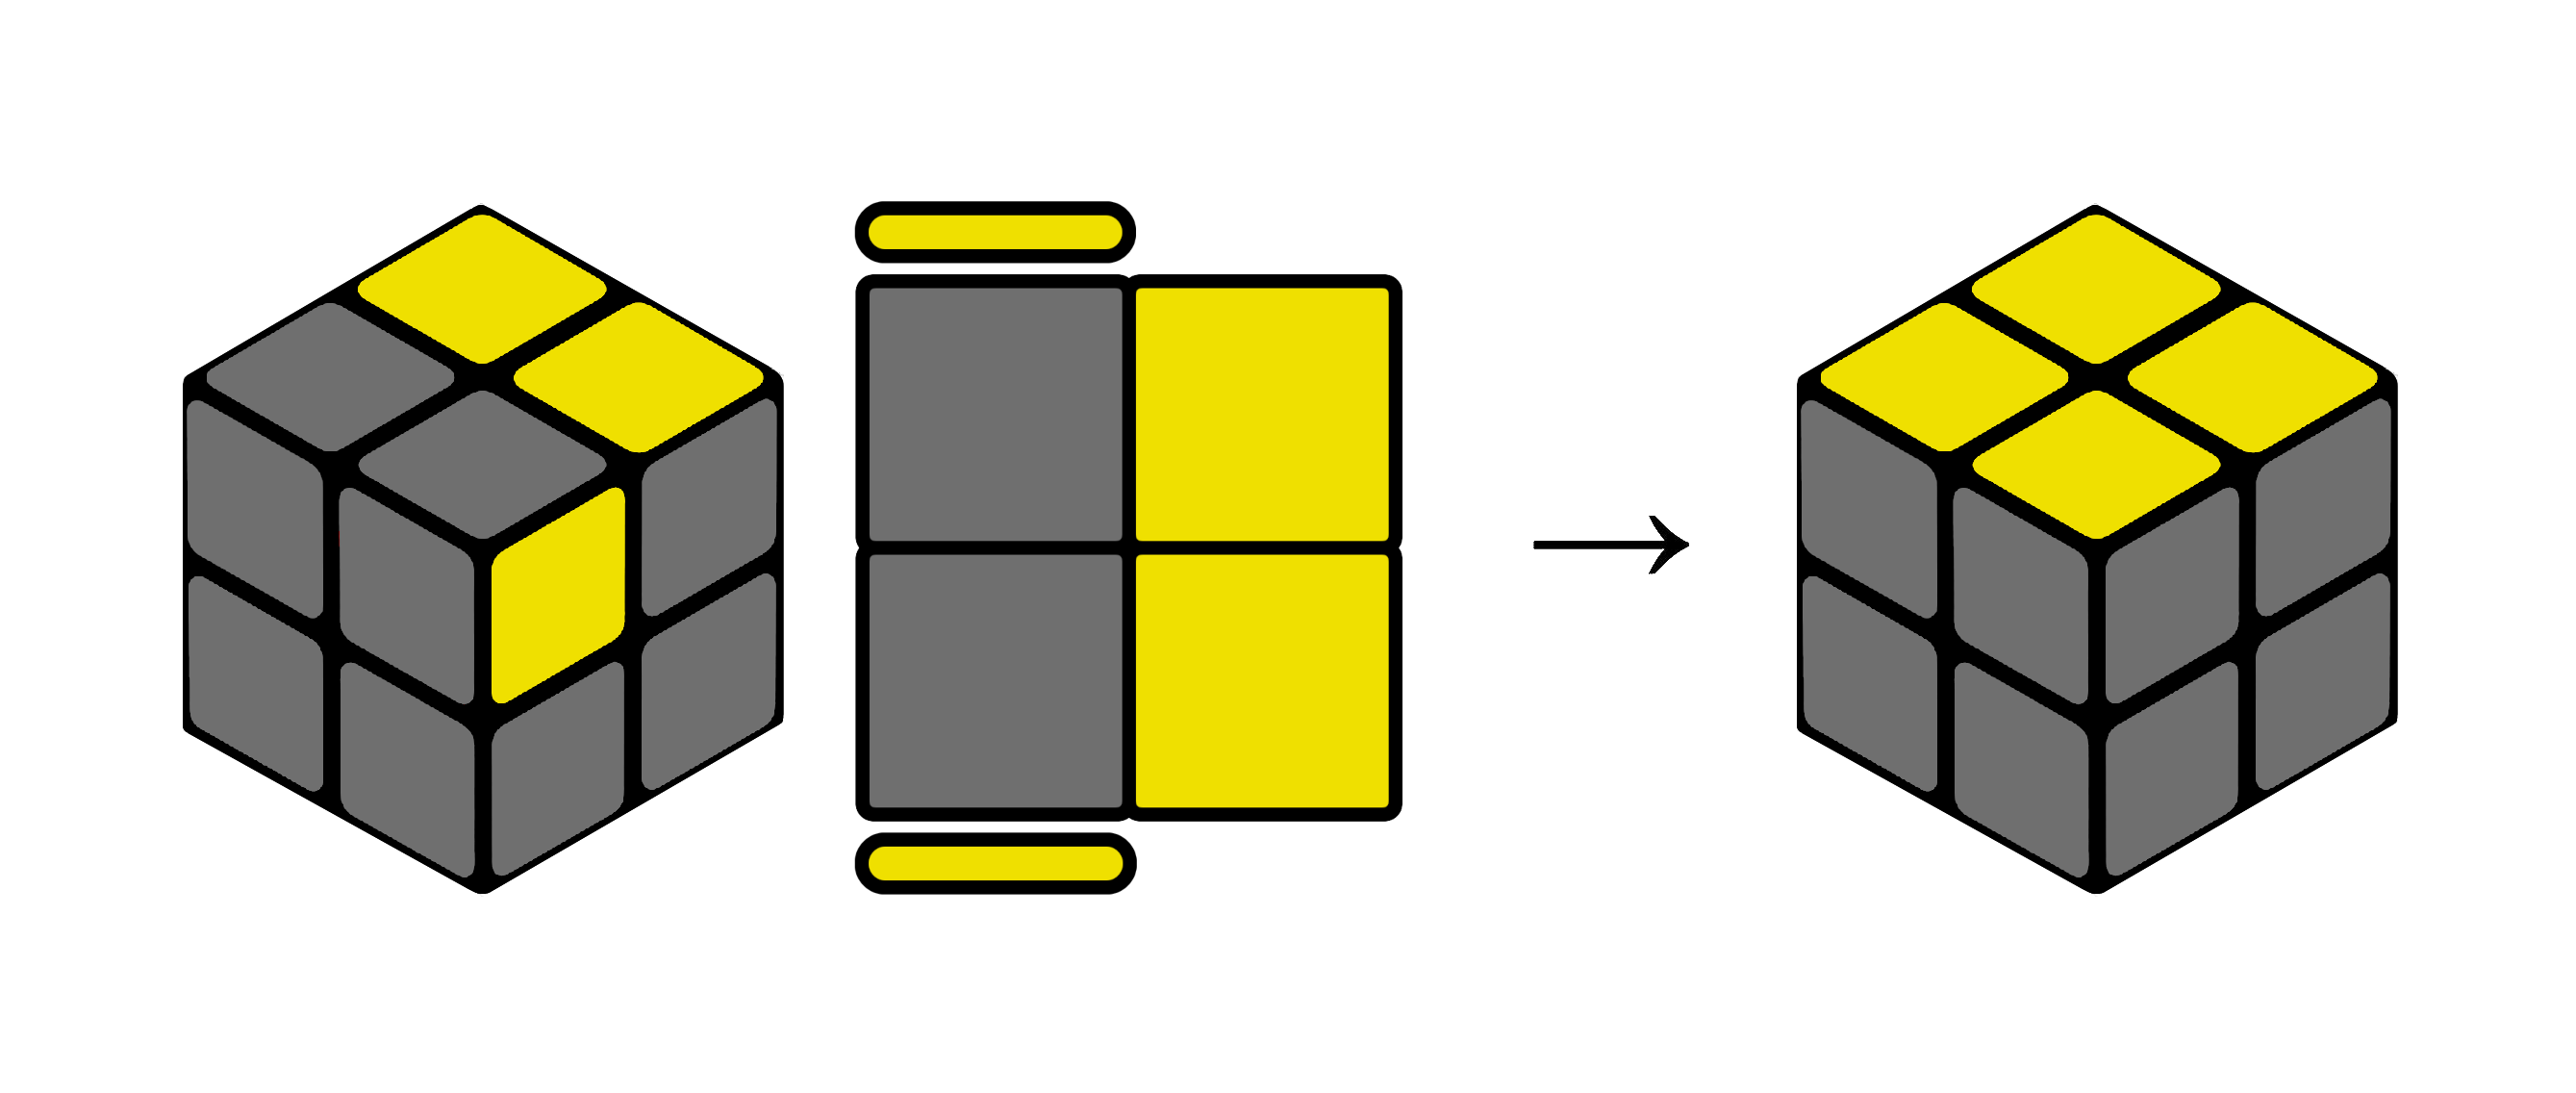
\includegraphics[scale=0.12]{isiakanm.png}
\caption{Ausrichtung der zweiten Ebene (Beispiel)}
\label{Abbildung_AusrichtungEbene2}
\end{figure}

$\lbrack R, U \rbrack \lbrack R^{-1}, F \rbrack$ kann auch als Zykel geschrieben werden: $( \ \textit{ulb} \ \textit{ulf} \ \textit{urb} \ )$. 
%
%
%
%
%
%
%
%
%
%
%=======================================================================================================
%
%
%
%
%
%
%
%
%
%
\subsection*{Lösung des Würfels anhand eines Beispiels}\addcontentsline{toc}{subsection}{\protect\numberline{}Lösung des Würfels anhand eines Beispiels}

In diesem Beispiel (Abbildung \ref{Abbildung_LösungMensch0}) wird der Würfel mit dem Zug $FUBRF^{-1}$ verdreht und so gelöst, wie ein Mensch den \textit{Cube} lösen würde.
In der Abbildung wurde der Würfel noch um $180^\circ$ um die $z$-Achse rotiert.

\begin{figure}[H]
\centering
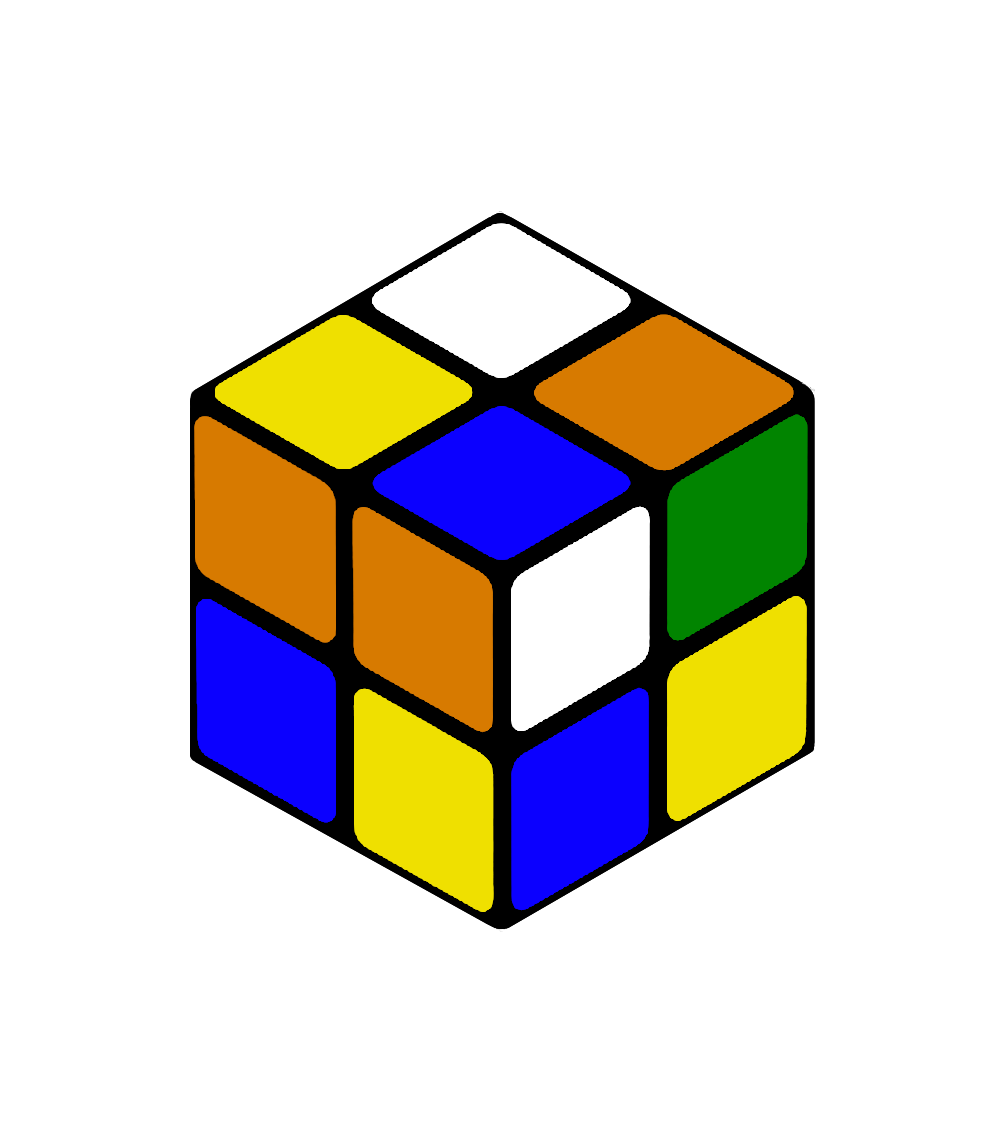
\includegraphics[scale=0.12]{LURFL1.png}
\caption{\textit{Cube} nach Zug $FUBRF^{-1}$ }
\label{Abbildung_LösungMensch0}
\end{figure}

Der erste Schritt für einen menschlichen Ansatz der Lösung des Würfels ist (meistens), die Steine der oberen Ebene so anzuordnen, dass die Farbflächen dort alle weiß sind und die vier oberen Steine in der richtigen Position zueinander sind. 
Für die Lösung der oberen muss $x_{1-4} = (0,0,0,0)$ gelten und $\sigma_{ulb}=\textit{ulb}, \  \sigma_{urb} = \textit{urb}, \  \sigma_{ulf} = \textit{ulf}, \  \sigma_{urf}=\textit{urf}$ bzw. die Äquivalenzklassen $\delta_{Z_r}$ und $\delta_{Z_l}$ davon. 

Der Lösende sucht nun Steine mit weißen Farbflächen und findet den weiß-orange-blauen Stein an der Position \textit{urf}. 
Mit dem Zug $F^{-1}$ findet der Stein seinen Platz in der oberen Ebene, mit der weißen Farbfläche oben. 
Nun ist $x_{1-4}=(0,2,0,1)$ und der Würfel sieht so aus, wie in Abbildung \ref{Abbildung_LösungMensch1} dargestellt: Es befinden sich nun zwei Steine der oberen Ebene an der richtigen Position -- der weiß-orange-blaue Stein und der weiß-rot-blaue Stein.

\begin{figure}[H]
\centering
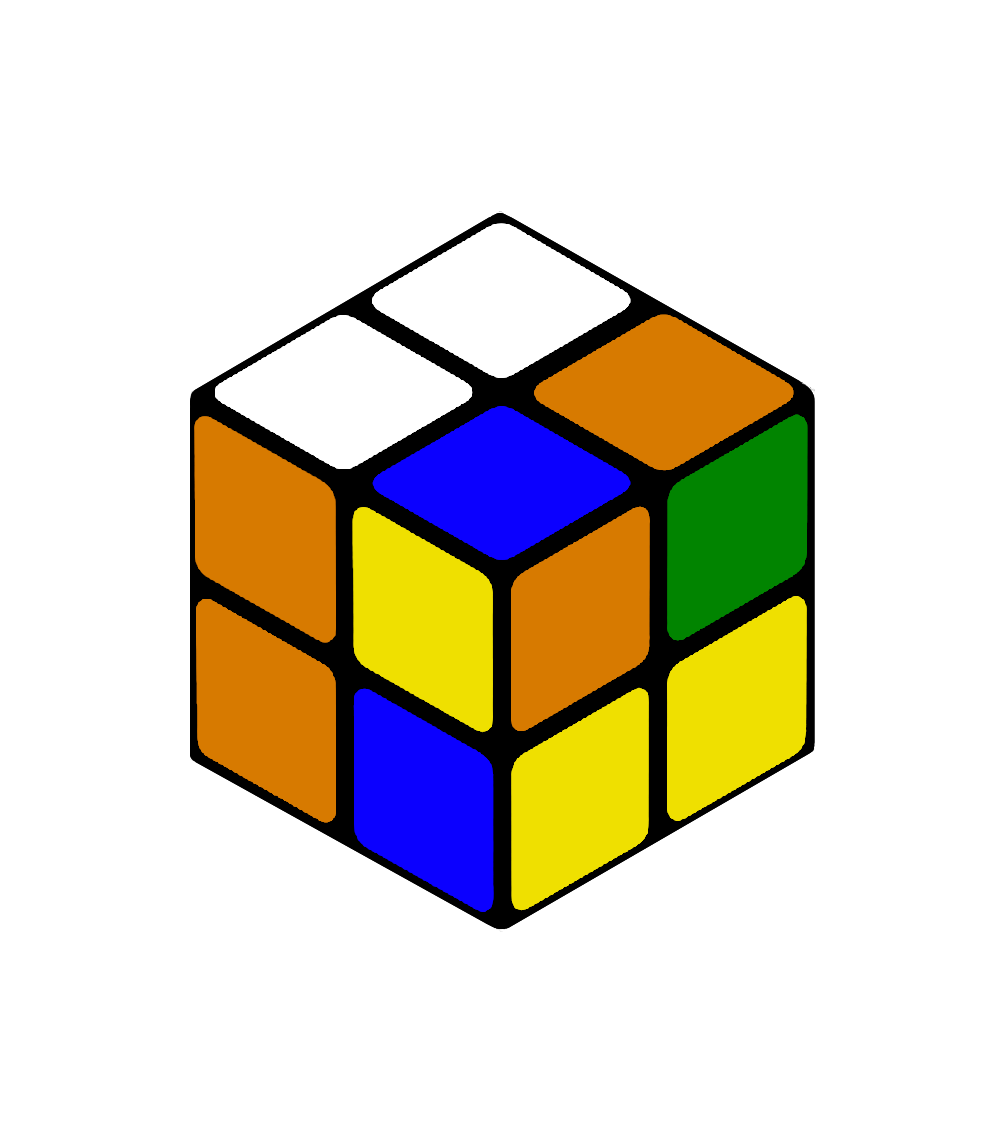
\includegraphics[scale=0.12]{0201.png}
\caption[Lösung von Mensch: Schritt 1]{Lösung von Mensch: Schritt 1}
\label{Abbildung_LösungMensch1}
\end{figure}

Der nächste Stein, der angeordnet wird, ist hier der weiß-grün-orange Stein. Er wird durch den Zug $R^{-1}$ in Position gebracht und findet seinen Platz neben dem weiß-orange-blauen Stein in der oberen Ebene (s. Abbildung \ref{Abbildung_LösungMensch2}).
 
\begin{figure}[H]
\centering
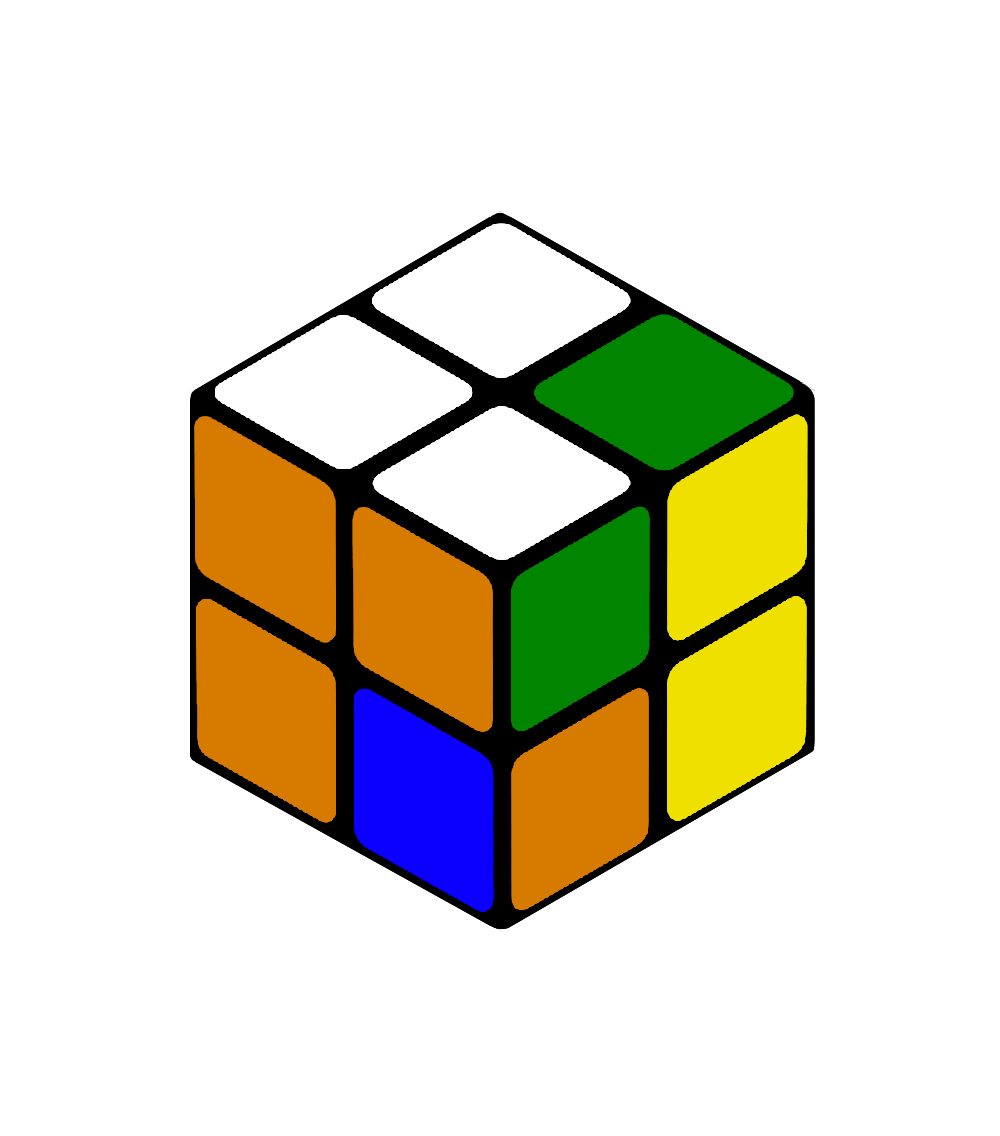
\includegraphics[scale=0.12]{menschSchritt2.png}
\caption[Lösung von Mensch: Schritt 2]{Lösung von Mensch: Schritt 2}
\label{Abbildung_LösungMensch2}
\end{figure}

Der letzte Stein mit weißer Farbfläche wird dann durch den Zug $RD^{-1}R^{-1}$ positioniert. Die obere Ebene ist nun gelöst und alle Steine mit weißen Farbflächen sind wie in der Startkonfiguration zueinander ausgerichtet. (s. Abbildung \ref{Abbildung_LösungMensch3}).
Dann gilt $x_{1-4} = (0,0,0,0)$ und durch die Äquivalenzklassen $\delta_{Z_r}$ oder $\delta_{Z_l}$ ist zu sehen, dass die Steine der oberen Ebene richtig zueinander angeordnet sind. Sie sind aber um $180^\circ$ gedreht zur Startkonfiguration. 

\begin{figure}[H]
\centering
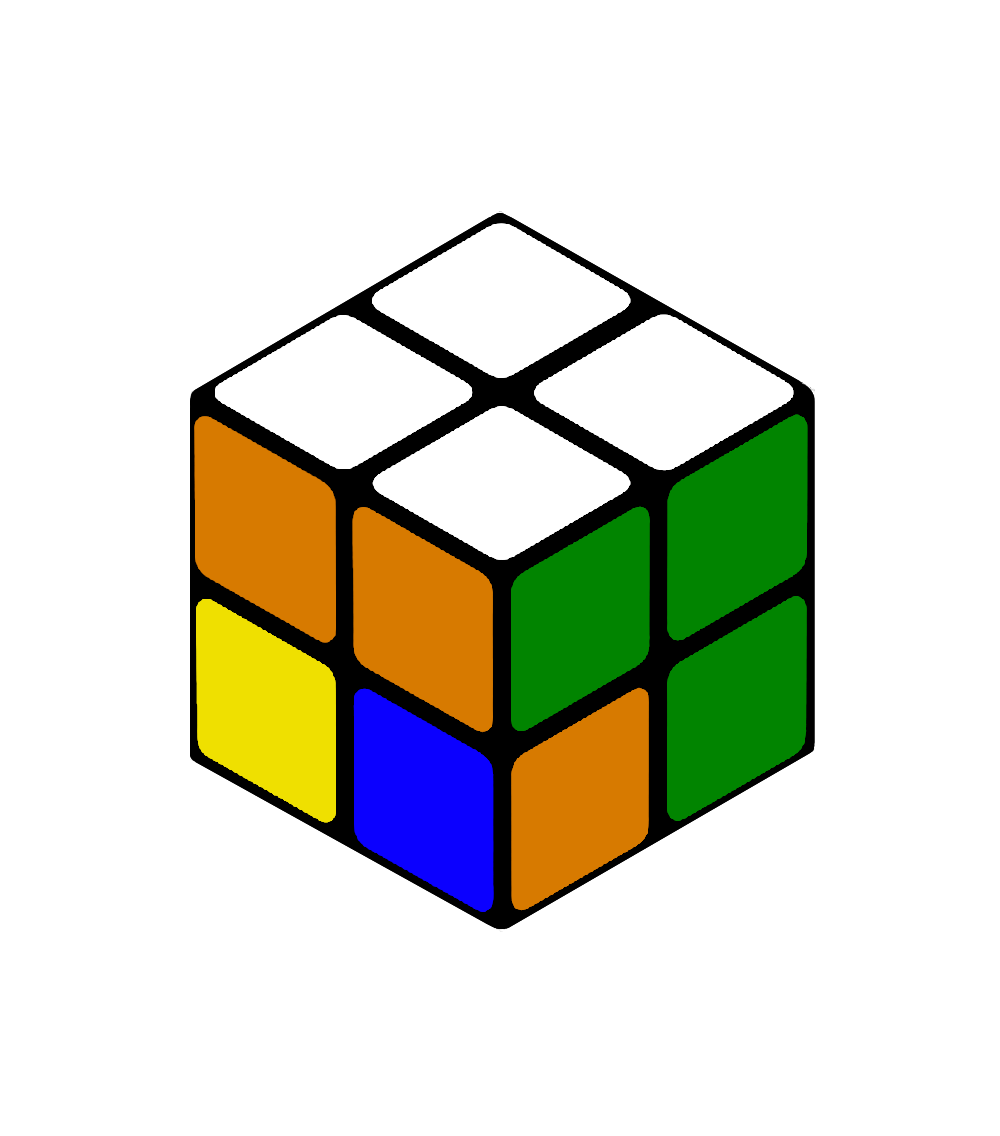
\includegraphics[scale=0.12]{menschSchritt3.png}
\caption[Lösung von Mensch: Schritt 3]{Lösung von Mensch: Schritt 3}
\label{Abbildung_LösungMensch3}
\end{figure} 

Für den nächsten Schritt rotiert der Mensch den Würfel, hier um die $y$-Achse (s. Abbildung \ref{Abbildung_LösungMensch4}). Die weiße Seite ist nun unten und zwei der vier gelben Farbflächen sind nach oben ausgerichtet.

\begin{figure}[H]
\centering
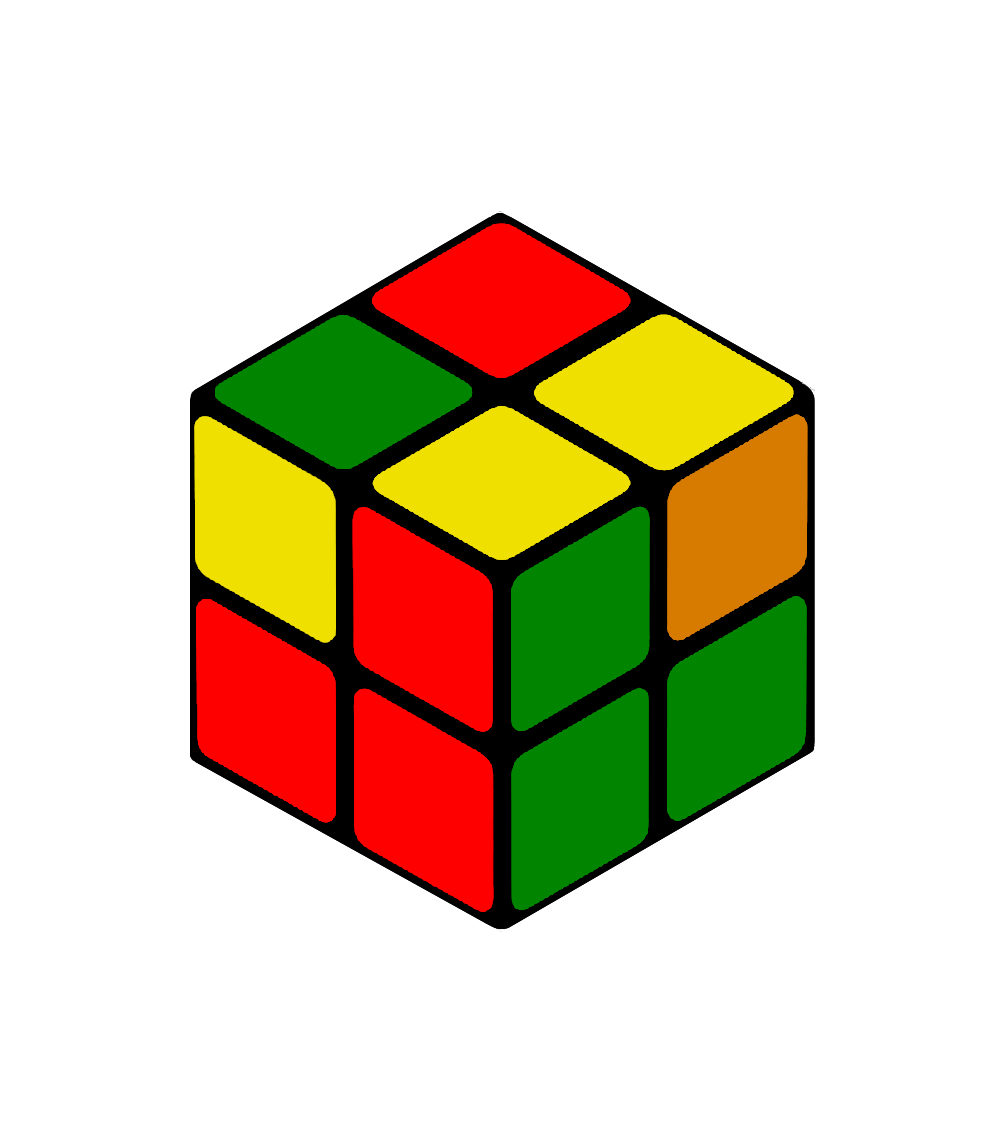
\includegraphics[scale=0.12]{menschSchritt4.png}
\caption[Lösung von Mensch: Schritt 4]{Lösung von Mensch: Schritt 4}
\label{Abbildung_LösungMensch4}
\end{figure} 

Dann führt der Lösende den Zug $RUR^{-1}U^{-1} \ R^{-1}FRF^{-1}$ aus \cite{RF2} und erhält einen gelösten Würfel (s. Abbildung \ref{Abbildung_LösungMensch5}). 

\begin{figure}[H]
\centering
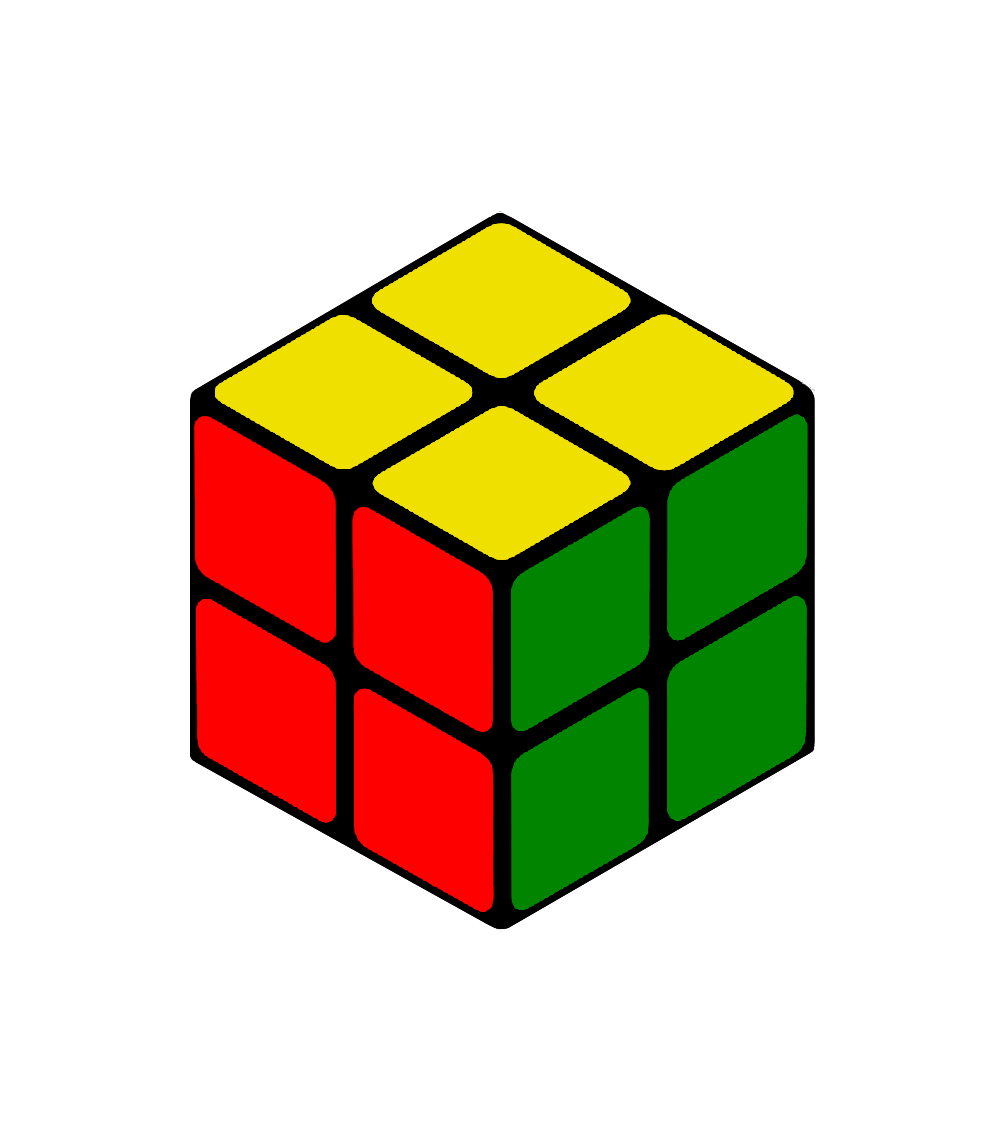
\includegraphics[scale=0.12]{menschSchritt5.png}
\caption[Lösung von Mensch: Schritt 5]{Der \textit{Cube} ist gelöst, die weiße Seite ist unten.}
\label{Abbildung_LösungMensch5}
\end{figure}

Der Mensch folgt beim Lösen des \textit{Cubes} (meistens) bestimmten Kombinationen, die in verschiedenen Situtionen anwendet werden können.  
In diesem Fall hat der Mensch $13$ Ebenen gedreht, während das Verdrehen nur $5$ Ebenenrotationen benötigte. Der Mensch hat folglich nicht den kürzesten Weg gewählt, aber dafür einen Weg, den er bei verschiedenen Würfelkonfiguratonen anpassen und verwenden kann. 
Wenn die Verdrehung des Würfels invertiert wird ($(FUBRF^{-1})^{-1}$), ergibt das die Kombination $FR^{-1}B^{-1}U^{-1}F^{-1}$, um den Würfel zu lösen.


Es stellt sich die Frage, wie viele Ebenendrehungen der \Ttwo Würfel maximal von der Lösung entfernt sein kann. Diese Zahl wird auch \textit{God's Number} genannt. \\ 
Bei einer Ebenendrehung werden die Ebenen um $90^\circ$ gedreht. Eine Ebenendrehung um $180^\circ$ wird als zwei Vierteldrehungen gewertet. Das wird \textit{Quarter-Turn} Metrik genannt. Es gibt noch andere Metriken, wie z.B. die \textit{Half-Turn} Metrik, bei der eine Drehung der Ebene um $90^\circ$ oder um $180^\circ$ als eine Drehung gezählt werden \cite{TR}.
Wenn in der \textit{Quarter-Turn} Metrik gerechnet wird, ist die \textit{God's Number} des \Ttwo Würfels $14$ \cite{DJ}.


%
%
%
%
%
%
%
%
%
%=======================================================================================================
%
%
%
%
%
%
%
%
%
%
\subsection*{Muster}\addcontentsline{toc}{subsection}{\protect\numberline{}Muster}
Dieser Abschnitt ist inspiriert von dem Part \textit{Pretty Patterns} in Tom Davis' \textit{Group Theory via Rubik's Cube} \cite{TD}.
Dort zeigt er einige \textit{hübsche} Muster des \Tthree Würfels und hier werden nun einige Muster des \Ttwo Würfels gezeigt.
In Abbildung \ref{Abbildung_Muster} werden vier Muster des \textit{Cubes} gezeigt und die dazugehörigen Algorithmen von der Startkonfiguration ausgehend beschrieben.

\begin{figure}[h]
\centering
\begin{tabular}{cc}
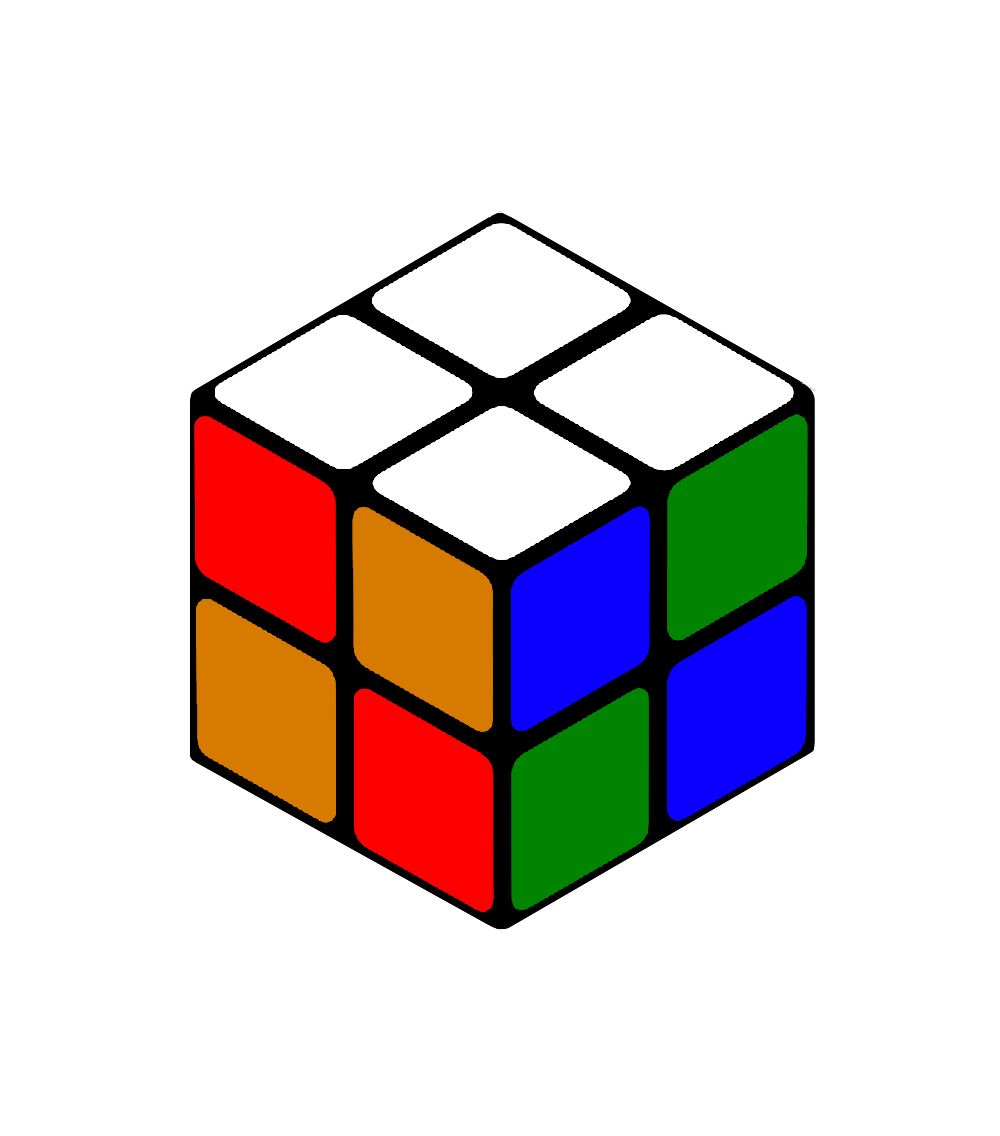
\includegraphics[scale=0.1]{RRFFRRUU.png} &  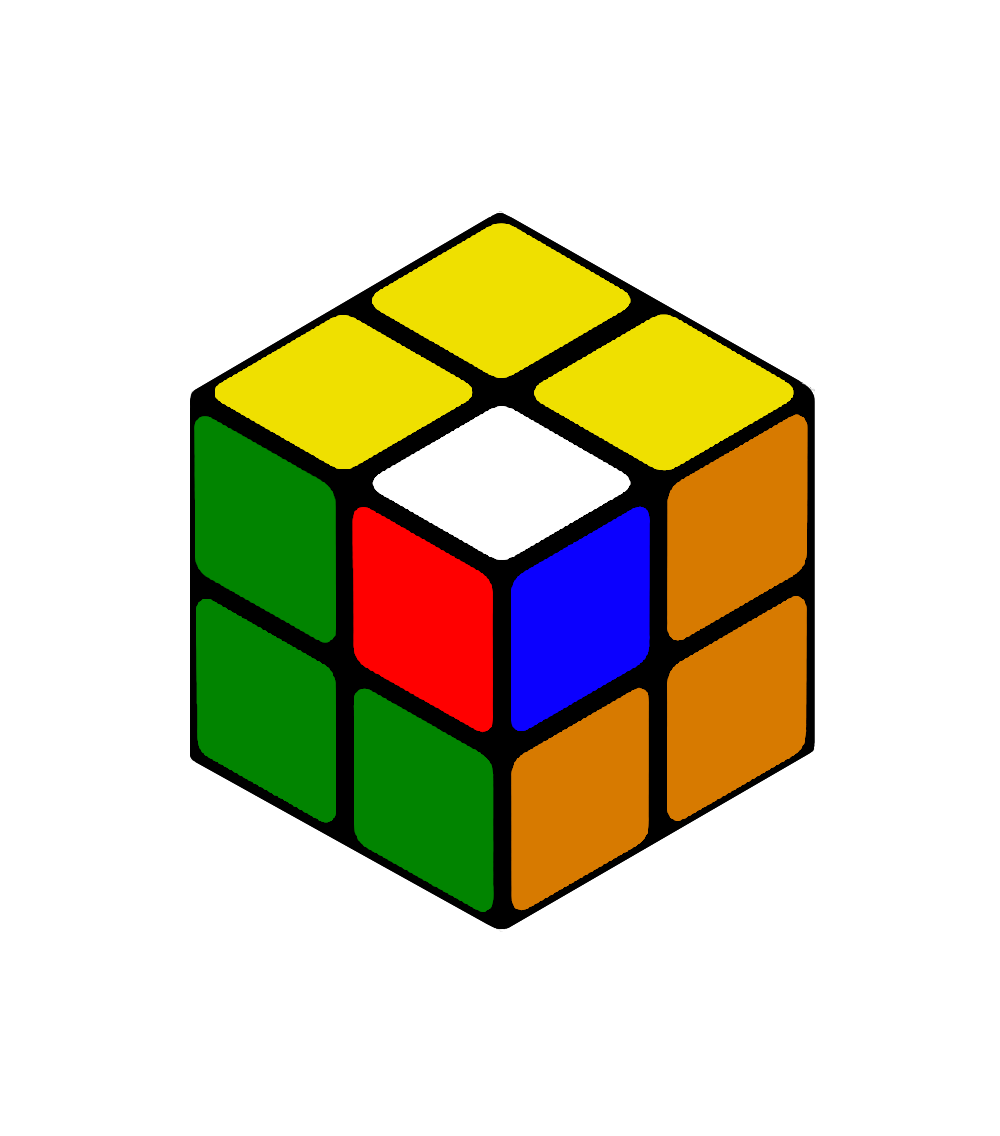
\includegraphics[scale=0.1]{CubeInCube.png} \\
Muster 1 & Muster 2 \\
$RR \ FF \, RR \ UU$ &  $R \ F \, U^{-1} \, RR \ U \, F^{-1} \, R \ U \, FF \, RR$ \\
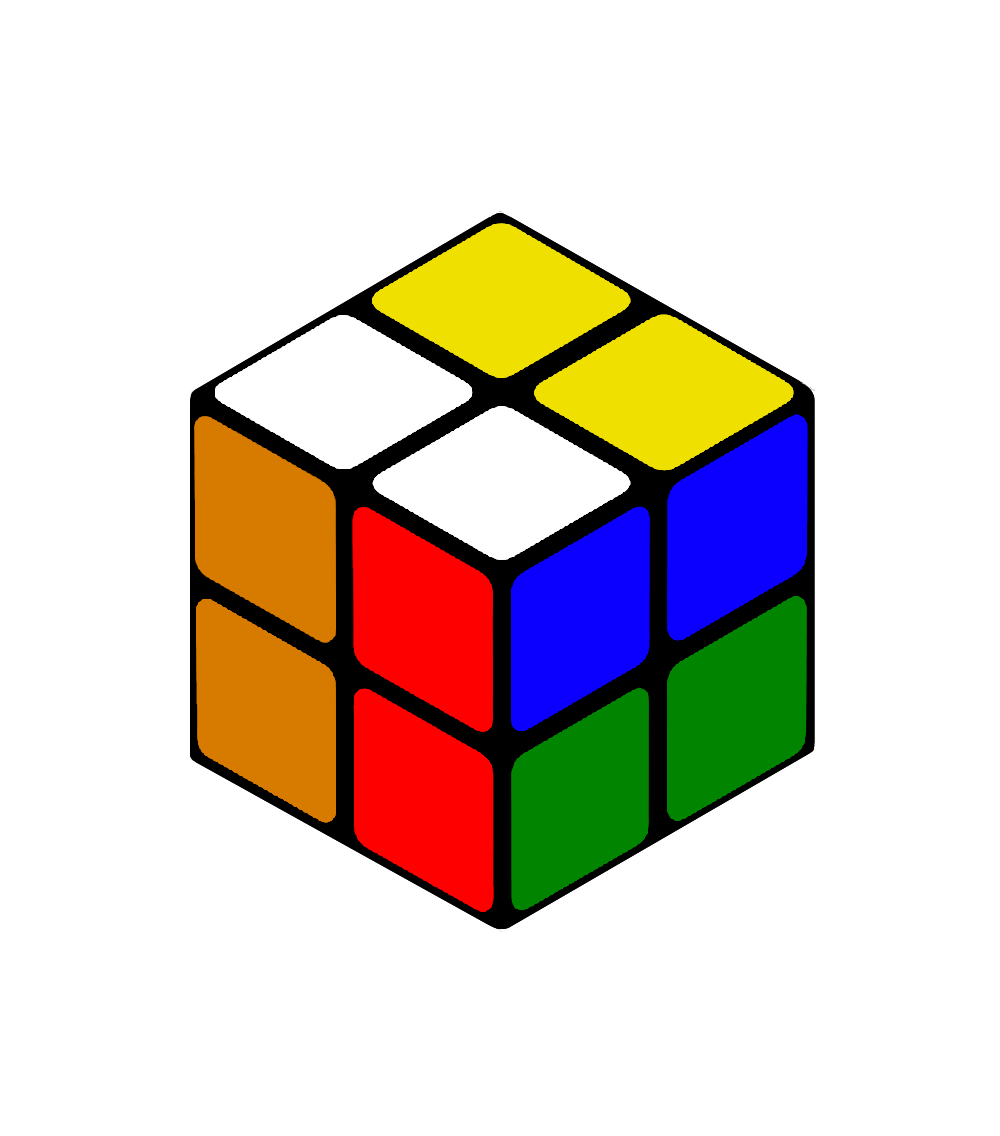
\includegraphics[scale=0.1]{UUFFRRUU.png} &  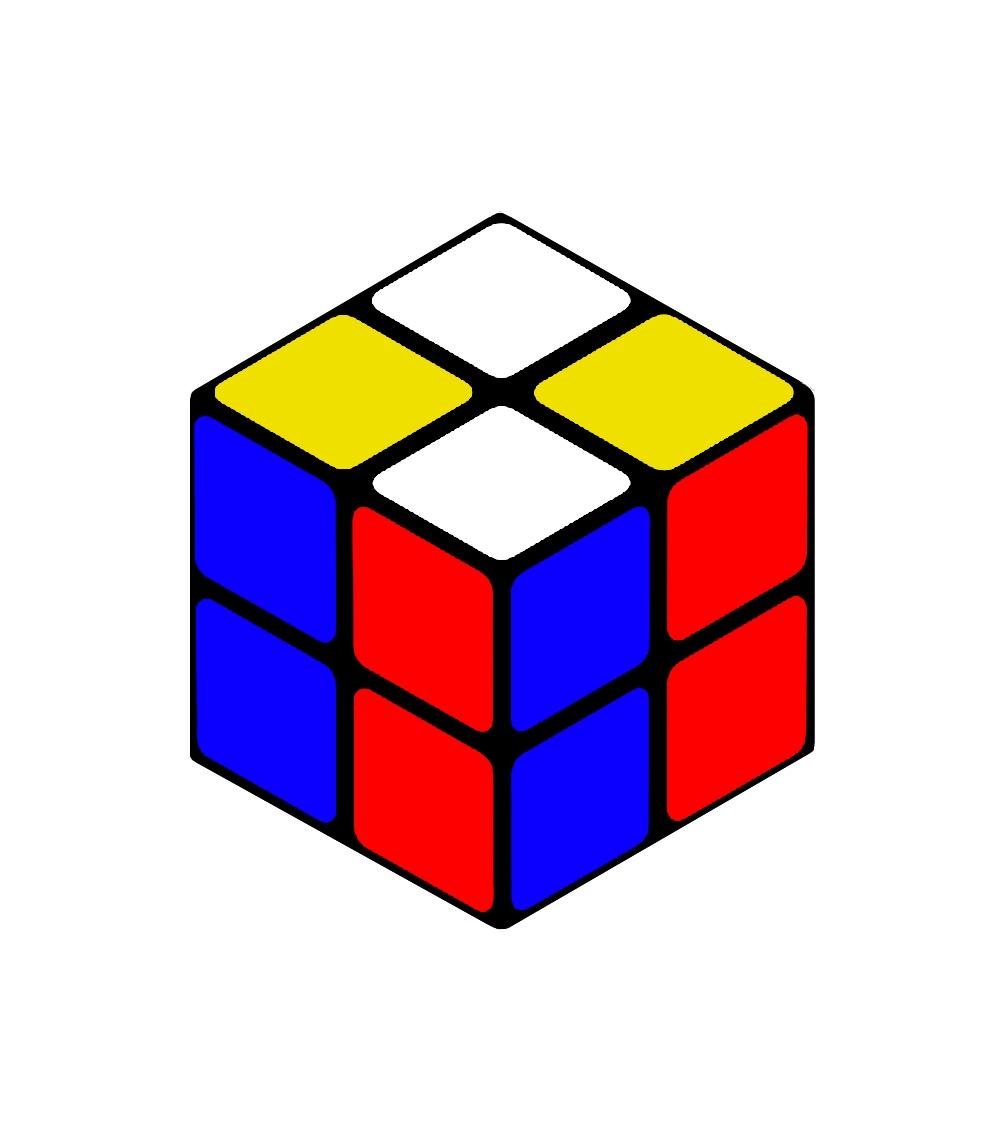
\includegraphics[scale=0.1]{UFFUURRU.png} \\
Muster 3 & Muster 4 \\
$UU \, FF \, RR \ UU$ &  $U \, FF \, UU \, RR \ U$ \\
\end{tabular}

\caption{Muster des \Ttwo Würfels}
\label{Abbildung_Muster}
\end{figure}

Muster 1 lässt die weiße und gelbe Seite unverändert und bildet ein Karomuster auf den anderen vier Seiten. Dabei werden die Farbpaare rot-orange und grün-blau zusammen im  Karomuster angeordnet.

Muster 2 hat einen \textit{Würfel im Würfel}. Dabei werden zwei Steine getauscht, die keine gemeinsame Farbfläche haben.

Muster 3 zeigt abwechselnd Quer- und Längsstreifen auf den verschiedenen Seiten.

Muster 4 ordnet die Farben wie vier Säulen an. Die weiße und die gelbe Seite ist dabei kariert, die anderen Seiten gestreift.


Diese Muster sind in den meisten Fällen zwar keine üblichen Lösungsalgorithmen, sollten aber in dieser Arbeit auch nicht unerwähnt bleiben.

%
%
%
%
%
%
%
%
%
%=======================================================================================================
%
%
%
%
%
%
%
%
%
%
\subsection*{Schraubendrehermethode}\addcontentsline{toc}{subsection}{\protect\numberline{}Schraubendrehermethode}

Die Methode, die oft als einfachste Methode zum Lösen von Zauberwürfeln beschrieben wird, ist die Schraubendrehermethode.
Bei den üblichen \Ttwo Würfel ist auf einer oder mehreren Seiten in der Mitte zwischen den Steinen eine Schraube zu sehen.
Um den Würfel auseinander zu bauen, muss diese Schrauben gelockert werden. Daraufhin kann die Ebene ohne Probleme abgenommen werden. 
Dann werden die Steine neu arrangiert und der Würfel kann in der gelösten Konfiguration wieder zusammen gebaut werden.

Ob das wirklich die einfachste Methode ist, liegt wohl im Auge des Betrachters und unter Berücksichtigung der Tatsache, dass der Weltrekord des \Ttwo Würfels mit der Methode des algorithmischen, händischen Lösens bei $0,49$ Sekunden liegt \cite{rekord}, ist die Schraubendrehermethode wohl kaum die schnellste Methode.

%
%
%
%
%
%
%
%
%
%=======================================================================================================
%
%
%
%
%
%
%
%
%
%
\subsection*{Algorithmen für die erste Ebene}\addcontentsline{toc}{subsection}{\protect\numberline{}Algorithmen für die erste Ebene}


Da der \Ttwo im Gegensatz zum \Tthree Würfel keine Mittelsteine hat, kann der erste Eckstein als richtig angenommen werden, da der Würfel nur gedreht werden muss, um eine weiße Farbfläche zu finden.
In diesen Beschreibungen wird sich an die Konvention gehalten, mit der weißen Seite oben zu beginnen. Es kann aber natürlich mit jeder anderen Seite des Würfels auch begonnen werden.
Der \Tthree \textit{Cube} muss entsprechend der Mittelsteine ausgerichtet werden und so ist vorbestimmt, welche Seite die weiße Seite wird, je nach Ausrichtung der Mittelsteine. Bei dem \Ttwo \textit{Cube} kann mit jeder beliebigen Seite begonnen werden. Wenn unbedingt mit einer bestimmten Seite als Oberseiten begonnen werden soll, die noch keine weiße Farbfläche hat, so kann die Farbfläche durch maximal zwei Ebenendrehungen an diese Seite gebracht werden.

In Abbildung \ref{Abbildung_ErsterEckstein} wird der erste Eckstein der oberen Ebene positioniert. Das kann dort entweder durch den Zug $R$ oder einer Rotation um die $y$-Achse passieren.

\begin{figure}[H]
\centering
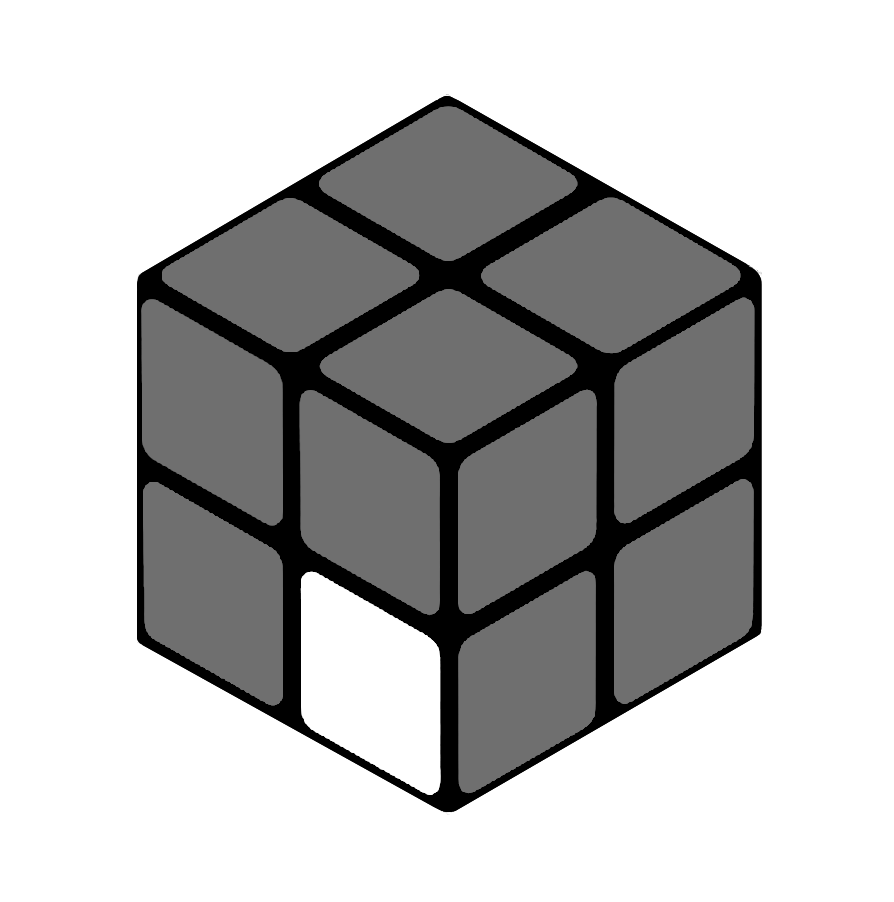
\includegraphics[scale=0.1]{e1_s1_s1.png}
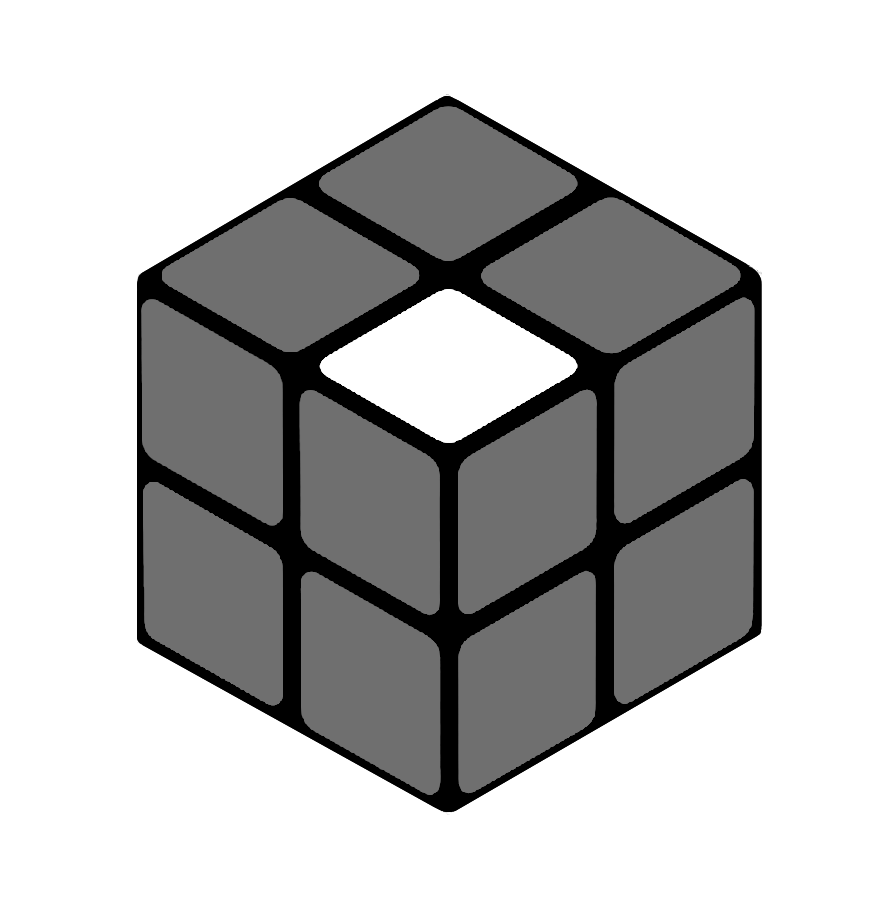
\includegraphics[scale=0.1]{e1_s1_s2.png}
\caption{ersten Eckstein positionieren}
\label{Abbildung_ErsterEckstein}
\end{figure}

Der zweite Stein kann dann hinzugefügt werden. Es gibt für den \Ttwo Würfel Lösungsmethoden, bei denen zuerst alle weißen Farbflächen ausgerichtet und dann die Steinposition anpasst werden.
Da hier aber Algorithmen des \Tthree Würfels übertragen werden, und bei diesem die Steine der oberen Ebene üblicherweise direkt richtig ausrichtet und positioniert werden, wird hier auch so vorgegangen.
Die Farbfläche des zweiten Steins befindet sich für diesen Algorithmus seitlich an der unteren Ebene. (Optimalerweise befindet sich der Stein schon zufällig an der gewünschten, korrekten Position.)
Dann wird $D$ ausgeführt, bis der Stein sich unter seiner Zielposition befindet und er wird mit $L, R, F$ oder $R$ neben den bereits vorhandenen ersten Eckstein gedreht. Das ist auch in Abbildung \ref{Abbildung_ZweiterEckstein} zu sehen.

\begin{figure}[H]
\centering
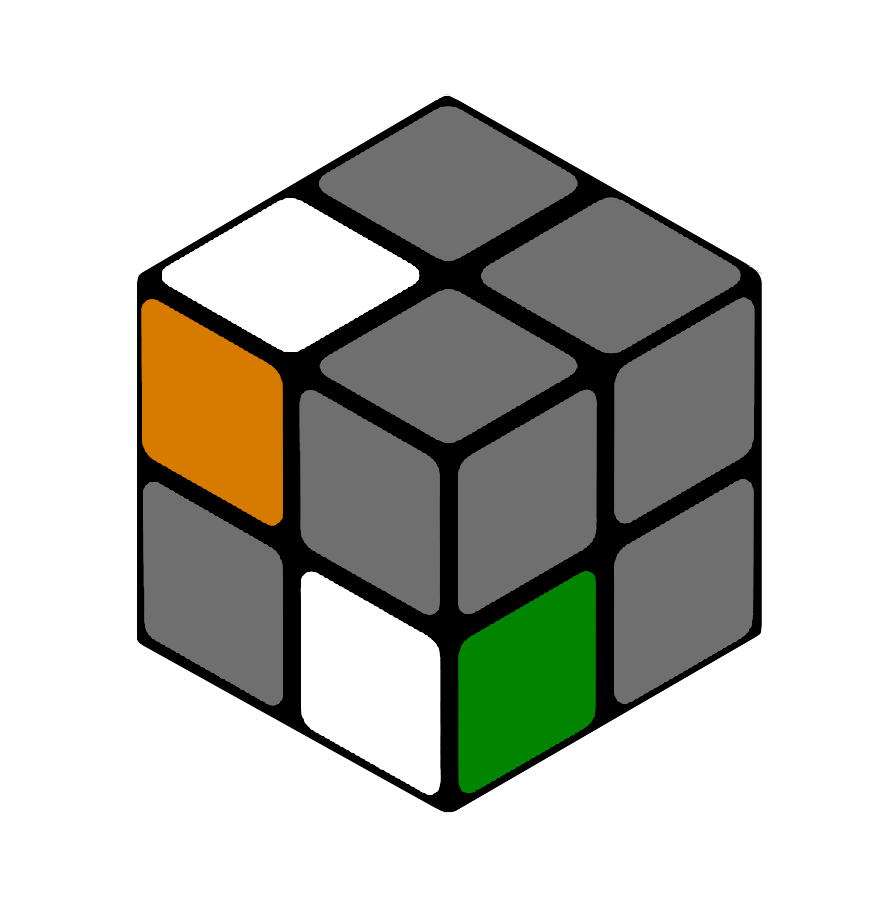
\includegraphics[scale=0.1]{e1_s2_s1.png}
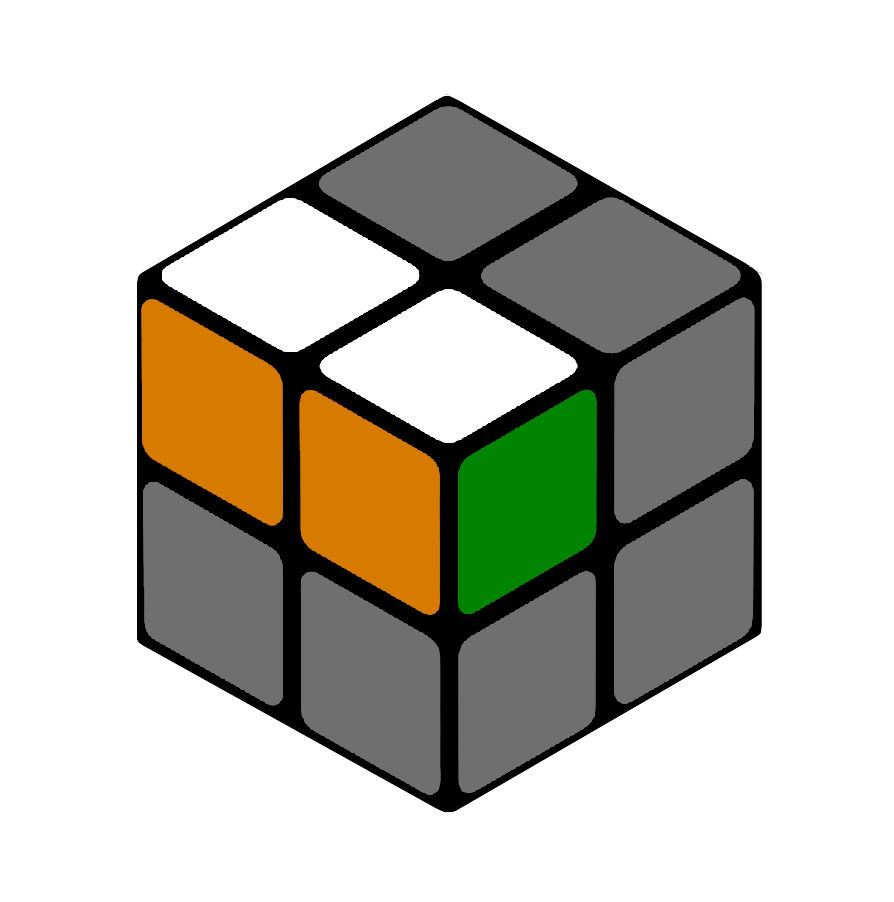
\includegraphics[scale=0.1]{e1_s2_s2.png}
\caption{zweiten Eckstein positionieren}
\label{Abbildung_ZweiterEckstein}
\end{figure}

Dort sind auch orange und grüne Farbflächen abgebildet. Das gilt analog für die anderen benachbarten Farbflächen. Wichtig ist, dass die beiden Farbflächen einer Seite auch die gleiche Farbe haben.

Sollte die weiße Farbfläche der Ecke unten am Würfel sein, so kann sie falsch herum ausgerichtet mit der Technik aus Abbildung \ref{Abbildung_ZweiterEckstein} an die Position gesetzt werden. Dann befindet sich die weiße Farbfläche in der oberen Ebene, aber falsch herum ausgerichtet. Wenn das der Fall ist, kann der Stein mit einem der Züge $L, R, F$ oder $B$ herausgedreht werden und mit $U$ in die untere Ebene geschoben werden. Dieser Vorgang ist auch in Abbildung \ref{Abbildung_ZweiterEckstein2} zu sehen. Von dort wird er mit der oben beschriebenen Technik richtig ausgerichtet und positioniert eingefügt (s. Abbildung \ref{Abbildung_ZweiterEckstein}). 

\begin{figure}[H]
\centering
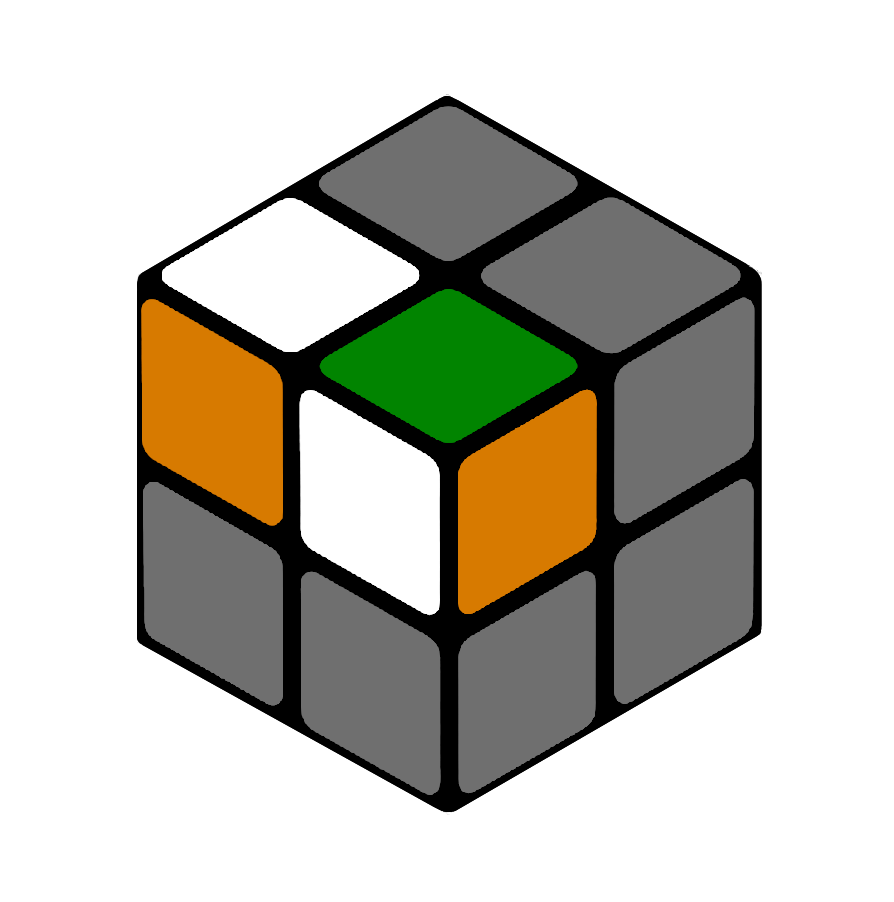
\includegraphics[scale=0.1]{e1_s2_s1_s.png}
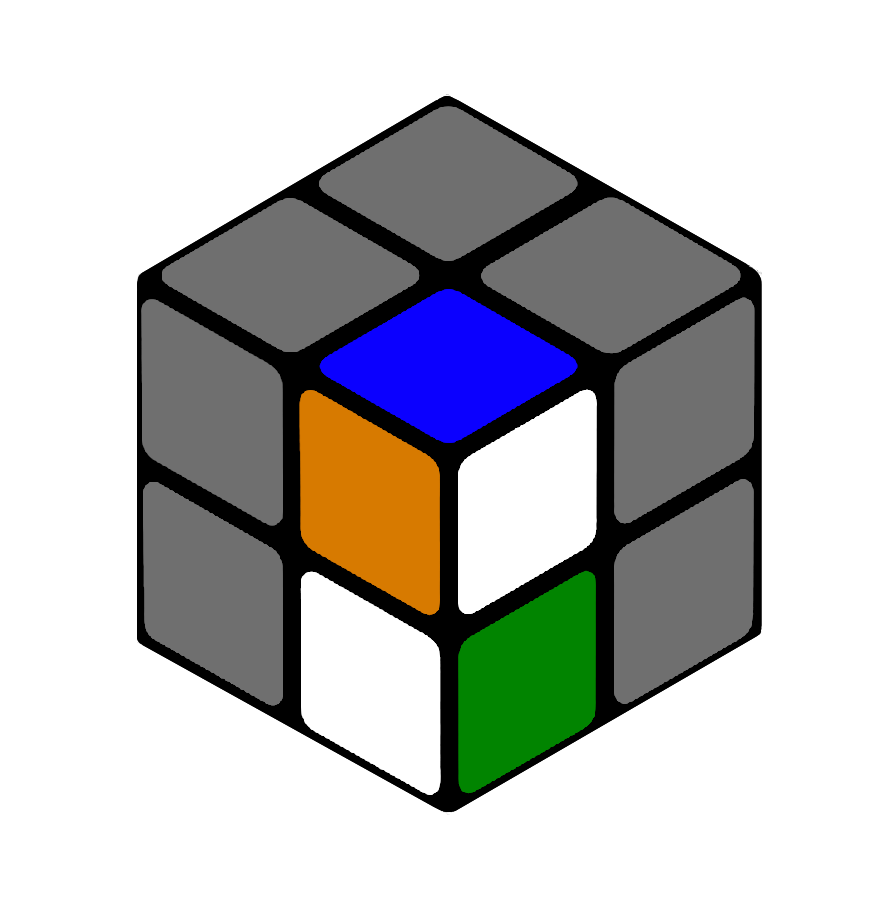
\includegraphics[scale=0.1]{e1_s2_s2_s.png}
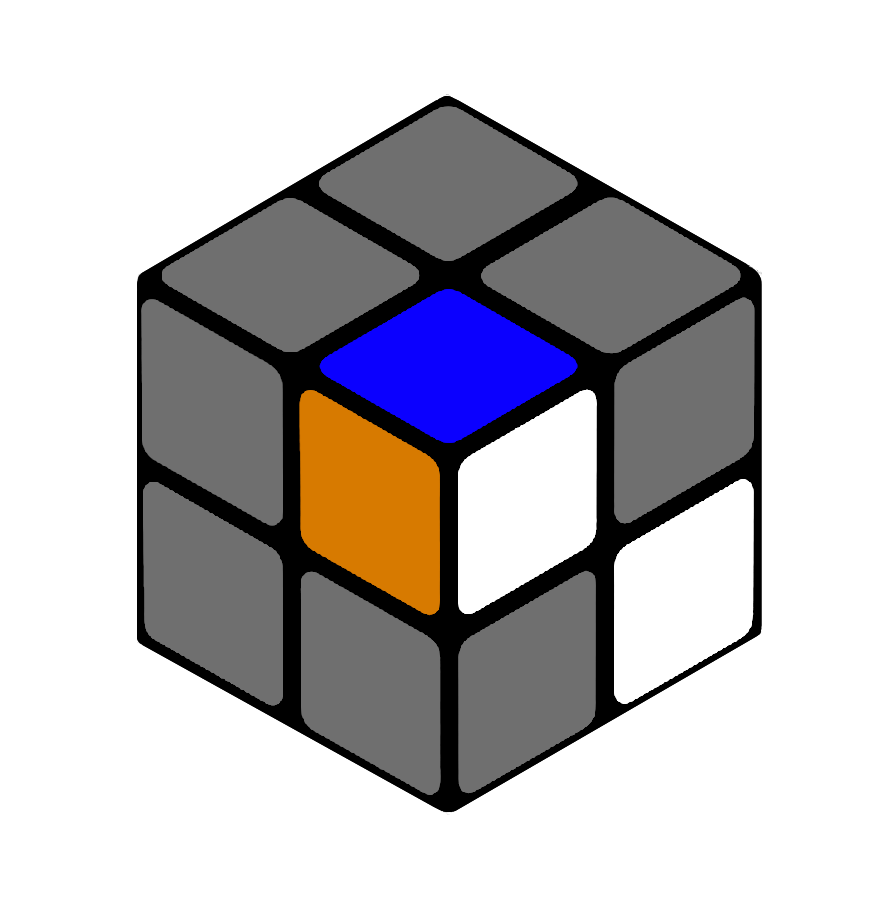
\includegraphics[scale=0.1]{e1_s2_s3_s.png}
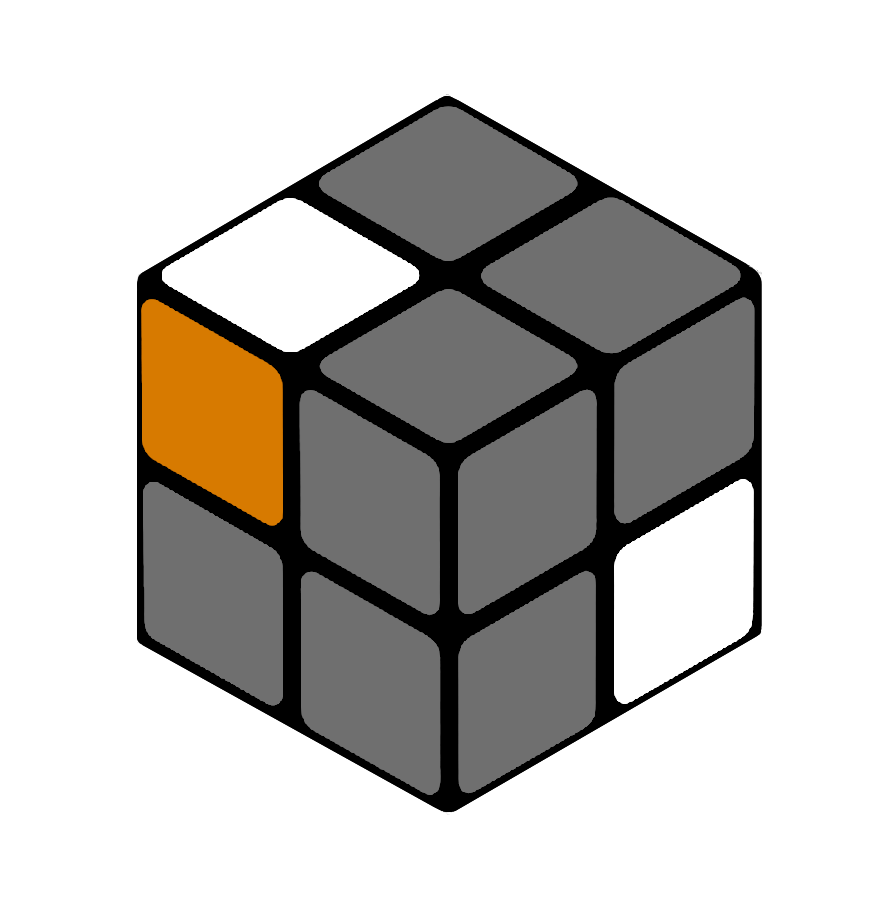
\includegraphics[scale=0.1]{e1_s2_s4_s.png}
\caption{zweiter Eckstein: Sonderfall}
\label{Abbildung_ZweiterEckstein2}
\end{figure}

Die anderen zwei Steine der ersten Ebene lassen sich mit der oben genannten Technik ebenfalls positionieren. Die obere Ebene ist dann gelöst.
Bei dem \Ttwo Würfel entspricht das Lösen der oberen Ebene sogar schon der Hälfte des Würfels.



%
%
%
%
%
%
%
%
%
%=======================================================================================================
%
%
%
%
%
%
%
%
%
%
\subsection*{Algorithmen für die zweite Ebene}\addcontentsline{toc}{subsection}{\protect\numberline{}Algorithmen für die zweite Ebene}

\begin{figure}[h]
\centering
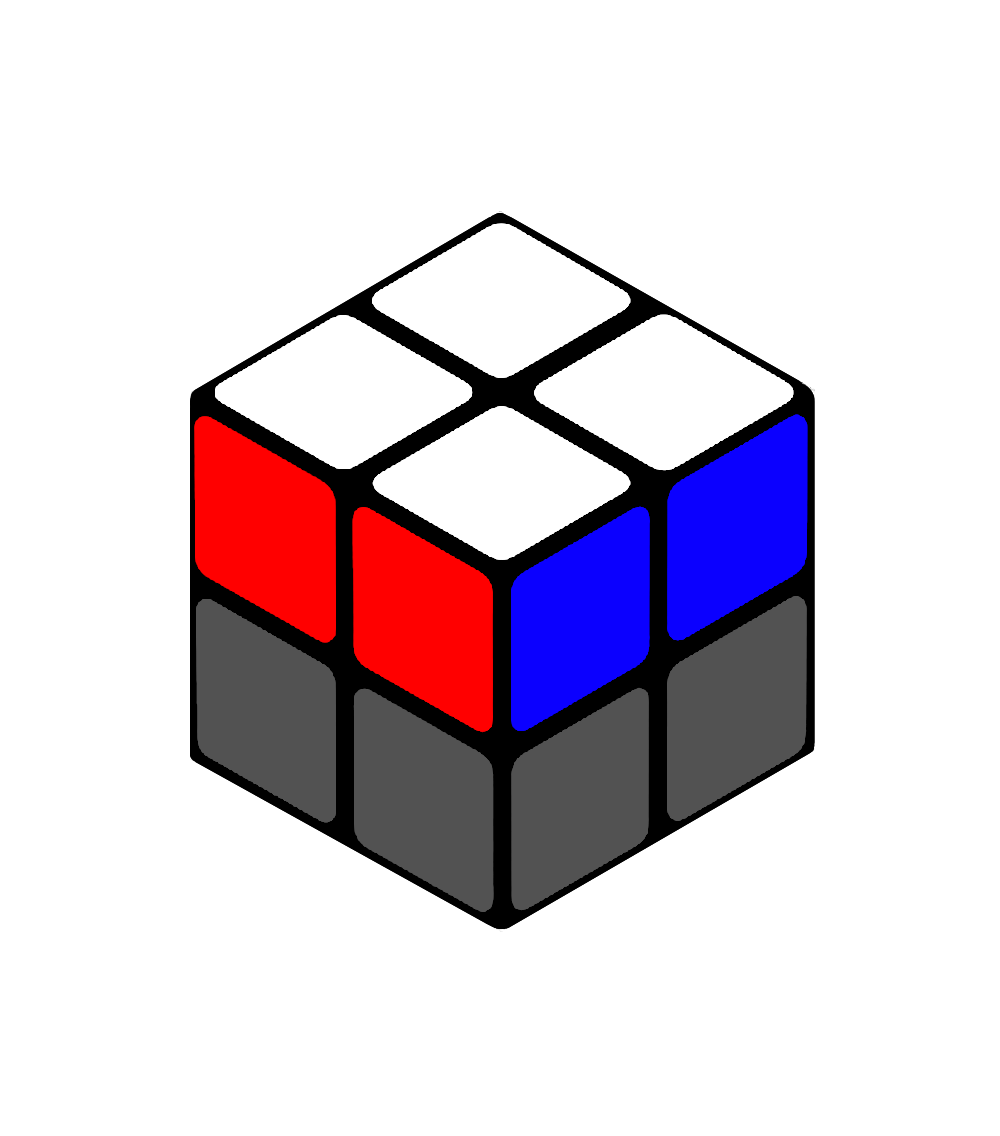
\includegraphics[scale=0.1]{ebene.png}
\caption{Würfel mit gelöster oberer Ebene}
\label{Abbildung_GelösteObereEbene}
\end{figure}

Beim Lösen der zweiten Ebene muss beachtet werden, die erste Ebene nicht wieder zu verdrehen. Deshalb sind die Algorithmen hier länger, um spezifische Steine zu bewegen.
In Abbildung \ref{Abbildung_GelösteObereEbene} ist die obere Ebene des Würfels gelöst.

Ein Mensch dreht zum Lösen der zweiten Ebene meistens den Würfel um. Der Anschaulichkeit halber wird das hier auch gemacht.

Zuerst werden nun alle Steine richtig ausgerichtet, so dass die obere Seite des Würfels nur noch gelbe Farbflächen zeigt. Dann werden die Steine getauscht, bis sie richtig angeordnet sind.

Da es auch nach Lösung der ersten Ebene noch viele mögliche Würfelkonfigurationen und Algorithmen zur Lösung dieser gibt, werden die möglichen Steinpositionen und Algorithmen in einer Tabelle aufgeführt. Die Algorithmen führen alle zu einer Würfelkonfiguration, bei der die untere (bereits gelöste) Ebene unverändert bleibt und die obere Seite nur gelbe Farbflächen zeigt.
Viele dieser Algorithmen enthalten $(R U R^{-1} U^{-1})$, was als Kommutator geschrieben $[ R,U ]$ ist.

\begin{center}
\begin{tabular}{m{4cm} m{6cm}}
\toprule
Ausgangsposition & Algorithmus  \\
\midrule
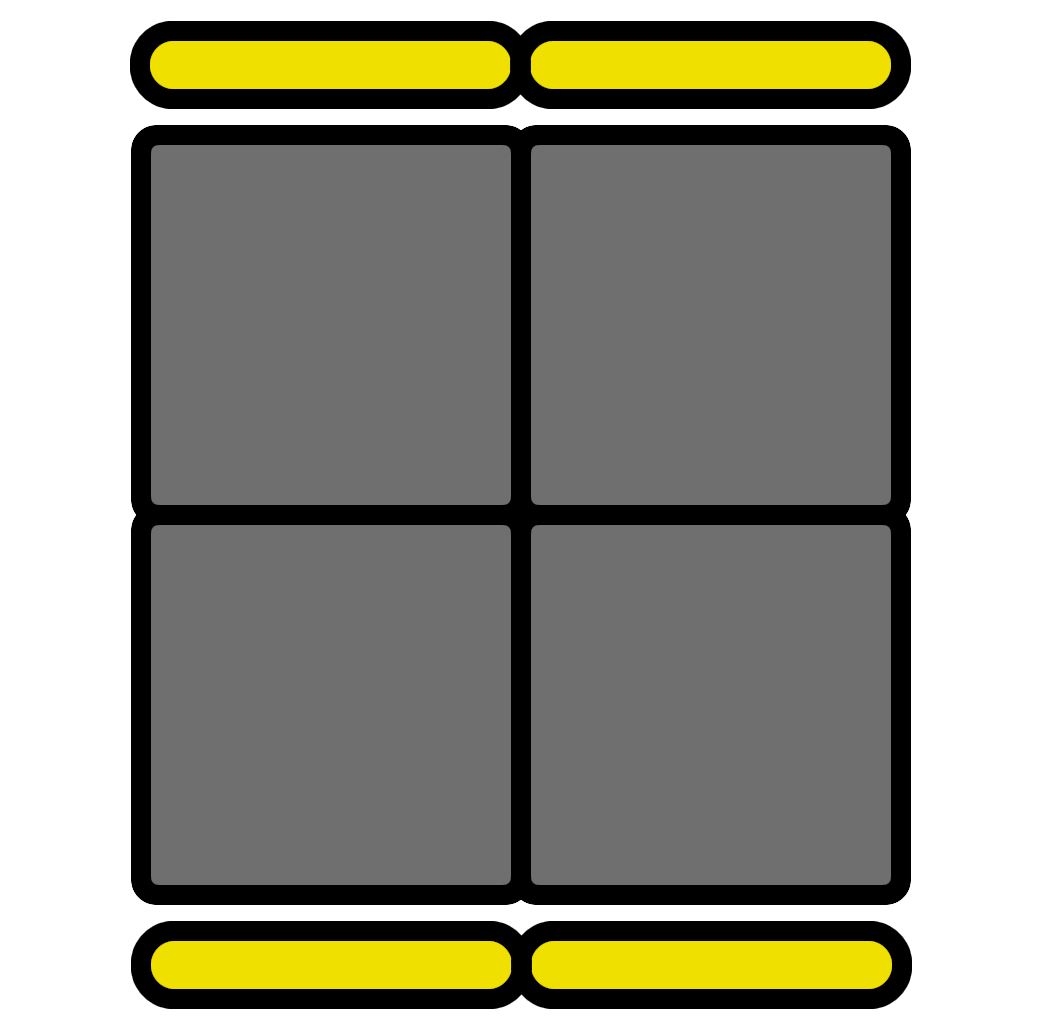
\includegraphics[scale=0.08]{TOPVIEW1.png} & $F \ [ R,U ] \  [ R,U ] \  [ R,U ] \ F^{-1}$ \\
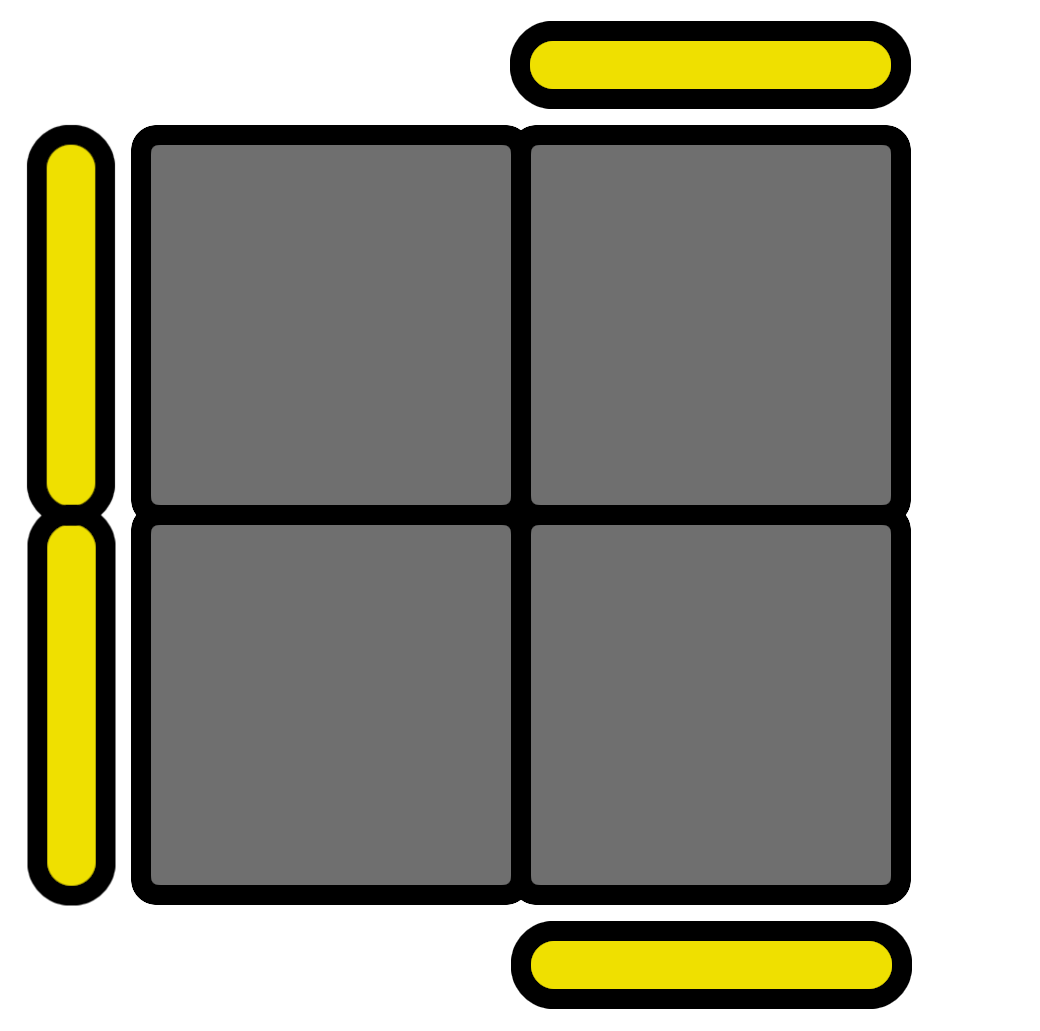
\includegraphics[scale=0.08]{TOPVIEW2.png} & $F \ [ R,U ] \  [ R,U ] \ F^{-1}$ \\
\includegraphics[scale=0.08]{TOPVIEW3_1.png} & $R \ U \ R^{-1} \ U \ R \ UU \ R^{-1}$ \\
\includegraphics[scale=0.08]{TOPVIEW3_2.png} & $L^{-1} \ U^{-1} L \ U^{-1} \ L^{-1} \ UU \ L$ \\
\includegraphics[scale=0.08]{TOPVIEW4.png} & $F \ [ R,U ] \ F^{-1}$ \\
\includegraphics[scale=0.08]{TOPVIEW5.png} & $[ R,U ] \ [R^{-1}, F]$ \\
\includegraphics[scale=0.08]{TOPVIEW6.png} & $F \ [ R,U ]\ R^{-1} \ F^{-1}\ R$ \\
\bottomrule
\end{tabular}
\end{center}


Die obere Seite des Würfels zeigt nach den Algorithmen nur noch gelbe Farbflächen. Die Ausrichtung der Steine ist dann bereits richtig. Wenn alle Steine der zweiten Ebene auch breits richtig zueiander angeordnet sind, muss die Ebene eventuell mit $U$, $U^{-1}$ oder $UU$ richtig zur ersten Ebene ausgerichtet werden.  Ansonsten werden die Steine getauscht, bis sie richtig angeordnet sind.

Zum Vertauschen der Steine untereinander (ohne die Ausrichtung zu verändern), gibt es auch wieder verschiedene Algorithmen. Diese Algorithmen werden hier in einer Liste aufgeführt, die Pfeile zeigen an, welche Steine beim Ausführen der Algorithmen an welche Würfelposition gelangen.

\begin{center}
\begin{tabular}{m{4cm} m{8cm}}
\toprule
Steinpermutation & Algorithmus  \\
\midrule
\includegraphics[scale=0.08]{corners1.png}  & $F \ R \ U^{-1} \ [R^{-1}, U^{-1}] \ R^{-1} \ F^{-1}  \ [R, U]   [R^{-1}, F]$ \\
\includegraphics[scale=0.08]{corners2.png}   & $[R,U] \  R^{-1} \ F \ RR \   U^{-1} \ [R^{-1}, U^{-1}] \ R^{-1} \  F^{-1})$ \\
\includegraphics[scale=0.08]{corners3.png}   & $R \ B^{-1} \ R \ FF \ R^{-1} \ B \ R \ FF \ RR $ \\
\bottomrule
\end{tabular}
\end{center}

Nach Wahl der passenden Algorithmen sollten beide Ebenen gelöst sein. Eventuell müssen die beiden Ebenen noch durch $U$, $U^{-1}$ oder $UU$ richtig zueinander ausgerichtet werden. Dann befindet sich der Würfel im gelösten Zustand.

%
%
%
%
%
%
%
%
%
%
%=======================================================================================================
%
%
%
%
%
%
%
%
%
%
\newpage


\section{Fazit}

\label{Kapitel_Fazit}


%
%
%
%
%
%
%
%
%
%
%=======================================================================================================
%
%
%
%
%
%
%
%
%
%
\subsection*{Zusammenfassung und Ergebnis}\addcontentsline{toc}{subsection}{\protect\numberline{}Zusammenfassung und Ergebnis}

In dieser Arbeit wurde die Gruppentheorie des \Tthree Würfels auf den \Ttwo Würfel übertragen, da der \Tthree \ im Gegensatz zum \Ttwo Würfel bereits oft untersucht wurde. Die Gruppe $(\Gtwo, \circ)$ des \Ttwo Würfels besteht aus der Menge aller Züge ($\Gtwo$) und dem Operator $\circ$, der zwei Züge aneinenader hängt. Die Mächtigkeit von $(\Gtwo, \circ)$ ist die Anzahl der validen Würfelkonfugurationen, also ist $|\Gtwo| = 3 \, 674 \, 160$. Die Rotation des kompletten Würfels wurde durch Äquivalenzrelationen realisiert. Außerdem wurden verschieden Lösungswege für den Würfel beschrieben und auf die \textit{God's Number} eingegangen. Diese ist beim \Ttwo Würfel $14$.

Die Gruppe des \Ttwo Würfels ist nützlich für die Veranschaulichung der Gruppentheorie an einem komplexen aber greifbaren Beispiel. Es können verschiedene Konzepte angewandt werden, wie Untergruppen, Erzeuger, zyklische Gruppen, Cayleygraphen, Gruppenoperationen, Kommutatoren, Äquivalenzrelationen, Mächtigkeit einer Gruppe, Ordnung von Gruppenelementen, Permutationen, Zykelschreibweise und symmetrische Gruppen.

%
%
%
%
%
%
%
%
%
%=======================================================================================================
%
%
%
%
%
%
%
%
%
%
\subsection*{Ausblick}\addcontentsline{toc}{subsection}{\protect\numberline{}Ausblick}

Es wurden in dieser Arbeit Erzeuger und deren Cayleygraphen der Gruppe $(\Gtwo, \circ)$ erwähnt. Weitere Cayleygraphen und Erzeuger der Gruppe des \Ttwo Würfels könnten durchaus interessant sein. Außerdem könnte eine \textit{GUI} zum Lösen des \Ttwo Würfels aufschlussreich sein, um effiziente Algorithmen zu finden und die Lösungswege des Würfels zu optimieren.
Auch wären weitere Untersuchungen der Gruppe $(\Gtwo, \circ)$ interessant, unter anderem die Berechnung der Anzahl der Isomorphismen, das Untersuchen der Gruppe auf Eigenschaften von Diedergruppen oder das Finden weiterer Untergruppen.
Ein weiterer sehr interessanter Aspekt ist das Finden eines Algorithmus, der die Gleichheit zweier Züge berechnet. Das kann mit einem Termersetzungssystem (\textit{Rewriting}) umgesetzt werden.

%
%
%
%
%
%
%
%
%
%=======================================================================================================
%
%
%
%
%
%
%
%
%
%
\newpage


\begin{singlespacing}
\listoffigures
\end{singlespacing}



\newpage

\begin{singlespacing}
\printbibliography
\end{singlespacing}








\end{document}














